\documentclass[11pt,a4paper]{article}
\usepackage[T1]{fontenc}
\usepackage[utf8]{inputenc}
\usepackage{lmodern}
\usepackage[margin=22mm]{geometry}
\usepackage{amsmath,amssymb,booktabs,tabularx,array}
\usepackage{enumitem,xcolor,tikz,xurl,hyperref}
\usetikzlibrary{arrows.meta,positioning,calc,fit}
\hypersetup{colorlinks=true,linkcolor=blue!55!black,urlcolor=blue!55!black,
  citecolor=blue!55!black,pdftitle={Abstract Machines: Steppers, Worlds and Semantic Connections}}
\setlength{\emergencystretch}{3em}
\setlength{\parskip}{5pt}
\setlength{\parindent}{0pt}
\setlist{nosep,leftmargin=*}
\definecolor{ink}{HTML}{18344D}
\definecolor{sea}{HTML}{087F8C}
\definecolor{amber}{HTML}{A86513}
\definecolor{pale}{HTML}{EDF5F8}
\tikzset{
  box/.style={draw=ink!65,fill=pale,rounded corners=2pt,align=center,
    text width=35mm,minimum height=13mm,inner sep=5pt,font=\small},
  wide/.style={box,text width=48mm},
  smallbox/.style={box,text width=27mm},
  future/.style={box,draw=amber,dashed,fill=amber!5},
  arr/.style={-{Stealth[length=2mm]},thick,draw=ink},
  hint/.style={font=\scriptsize,align=center,text=ink},
  boundary/.style={draw=amber,dashed,rounded corners,inner sep=7pt}
}
\newcommand{\code}[1]{\texttt{\detokenize{#1}}}
\newcommand{\name}[1]{\textup{\Urlmuskip=0mu\relax\nolinkurl{#1}}}
\newcommand{\sources}[1]{\par\smallskip{\small\raggedright\textbf{Existing owners.} #1\par}}
\newcommand{\scope}[1]{\par\smallskip\begin{quote}\small\textbf{Boundary.} #1\end{quote}}
\newcommand{\diagramcaption}[1]{\par{\small\color{ink}#1\par}\medskip}
\newcommand{\run}{\mathsf{run}}
\newcommand{\resume}{\mathsf{resume}}
\newcommand{\obs}{\mathsf{obs}}

\title{\color{ink}Abstract Machines\\[3pt]
  \large Steppers, retained worlds and semantic connections in Mettapedia}
\author{Mettapedia Working Notes}
\date{19 October 2026}

\begin{document}
\maketitle
\begin{abstract}
An abstract machine records unfinished work, its binding environment or world,
and the observations already committed. This overview distinguishes three
connections: independent language judgments, their retained operational
machines, and particular implementation realizations. Common finite-block
simulation and resumption laws support substantial CAM, fixed-C, HE and PeTTa
instances without identifying their languages or strategies. The principal
source correspondences, selected realization laws and their remaining gaps
are stated separately. Later sections discuss regional execution and proof
machines as applications and research directions; they do not enlarge the
finite abstract-machine acceptance boundary.
\end{abstract}

\section{One map, several machines}

The language rules say what a computation means. The machine says how its
unfinished work is represented. A VM additionally supplies a code image,
loader and instruction-admission contract. A native implementation must
realize those representations and transitions under its memory and service
assumptions. Each connection needs its own theorem or qualification evidence.
Section~\ref{sec:checking} develops the corresponding proof-checking machine:
what follows from what, under which conditions, and how its evidence composes.

\begin{center}
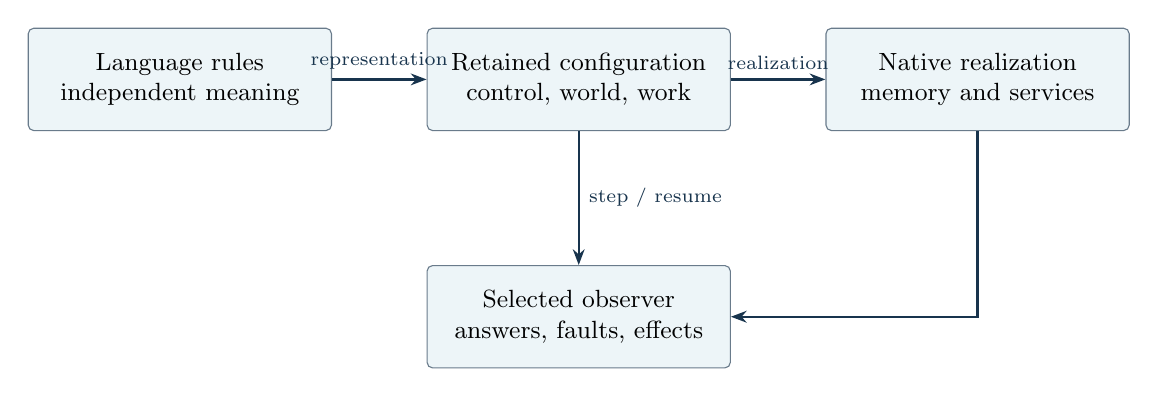
\begin{tikzpicture}
  \node[box] (source) {Language rules\\independent meaning};
  \node[box,right=12mm of source] (machine) {Retained configuration\\control, world, work};
  \node[box,right=12mm of machine] (native) {Native realization\\memory and services};
  \node[box,below=17mm of machine] (observer) {Selected observer\\answers, faults, effects};
  \draw[arr] (source) -- node[hint,above]{representation} (machine);
  \draw[arr] (machine) -- node[hint,above]{realization} (native);
  \draw[arr] (machine) -- node[hint,right]{step / resume} (observer);
  \draw[arr] (native.south) |- (observer.east);
\end{tikzpicture}
\end{center}
\diagramcaption{Similar outputs on examples test a connection. They do not replace a
general correspondence theorem between independently defined semantics.}

\begin{tabularx}{\linewidth}{@{}lX@{}}
\toprule
Family & Distinguishing retained information \\
\midrule
CEK / Krivine & Value environments and argument frames / unevaluated closures. \\
Categorical CAM & Register, compiled closures, remaining code and value stack. \\
HE & Typed/minimal work, scoped bindings, alternatives and return/collection boundaries. \\
PeTTa & Ordered control, bindings, saved callers, alternatives and collection scopes. \\
Branch-local Need & Cell origins, memo states, branch worlds and reuse identity. \\
Refocusing & Legal context stack, focused redex and ordered candidate attempts. \\
GSLT / rho & Scoped search jobs, unmet obligations and occurrence-bearing receipts. \\
C-language core & Byte memory, continuations, pending expression occurrences. \\
\bottomrule
\end{tabularx}

The historical \emph{Categorical Abstract Machine} and the machine for the
\emph{C language} are different instances. Neither supplies a universal fastest
strategy. The broader observer and logical-world foundation is developed in
\name{papers/metatheory.tex}.

The HE and PeTTa developments are further language instances, with their own
demand, return, search and publication rules. Changing a storage representation
changes its realization map. Changing a language rule changes its local
semantic obligations and can change program observations. The surrounding
execution and composition laws remain reusable where their hypotheses hold;
a shared interface does not identify the languages or their strategies.

The realization boundary is a binding store, retained control, occurrence
selection, world/services and publication. Their realization obligations are
local loading, step-block, readout and resumption laws on formal component models. Literal C
fragments and field inventories below are downstream worked examples; their
theorems do not by themselves connect a current source revision or a compiled
binary. No helper function or storage layout supplies the language semantics.

\subsection*{Profile taxonomy and the higher-order boundary}

The language-facing machines in this paper are explicit first-order Atom
profiles of existing dialects. HE's contextual machine observes completed
answers as a bag. Its plain-Atom first-success worker is a restricted
realization requiring closed type annotations and excluding held-readiness
reuse and embedded minimal instructions. The E1/E2 HE--PeTTa comparison admits
open recursion only through passive environments. PeTTa's \name{EagerDFS}
machine gives ordered, destination-scoped depth-first execution. These profiles
neither define MeTTa nor bound HO MeTTa Prime, whose machine must account for
binders, typed contexts and additional search strategies.

The HE M1--M8 component instance below has a deliberately narrower role: it
proves that changing the representation of a restored state does not change
the run of the same contextual rule. It is not an AM-to-native refinement. A
first cross-machine Prime instance awaits Prime's independently defined
machine.

\subsection*{Principal correspondences and explicit profiles}

The central distinction is
\[
 \text{independent source judgments}
 \;\longleftrightarrow\;
 \text{retained contextual machine}
 \;\longleftrightarrow\;
 \text{particular realization}.
\]
The two arrows have different invariants and different coverage. For HE,
\name{RecursiveExecution.Contextual.source_iff_observed} relates independent
completed source judgments to actual machine paths under arbitrary retained
callers and the declared lookup, dispatch and policy. Its public completion
observer is a bag of joint caller/value observations. The stronger comparison
with the plain-Atom worker in \name{FirstSuccessScopedAdequacy} has additional
entry, coverage and materialization obligations. Those obligations describe
that realization; they do not restrict the source language or replace the
already constructed source/contextual correspondence. Their general recursive
block composition is closed for the declared typed/cast/selection,
selected-function, tuple, ordinary-call and ranked-fallback worker profile.
Held readiness and embedded minimal instructions remain explicit negative
boundaries of that stripped representation; the contextual AM retains the full
grammar.

The HE \name{Completed.Policy} record selects reentry, marking, rebuilding and
matching. \code{unmarked}, \code{ready}, \code{unchangedReady} and
\code{finiteTypes} name local profiles, not whole-engine conformance claims.
Type enumeration is a separate explicit parameter: \name{TypeOccurrencesRel}
specifies the multiset of source occurrences, while \name{TypeEnumeration}
provides one complete, unique enumeration for each query. A first-success
consumer may observe that choice. Changing it therefore needs its local
semantic law; a bag observer does not make all first-success choices equal.

PeTTa's saturated-list evaluator and its scoped destination machine likewise
have separate source profiles. The latter retains open constraints, saved
callers, ordered alternatives, collection scopes and commit delimiters. Its
\name{Scoped.source_run_iff_derivation} compares actual finite execution with
independent source rules. Neither the former implementation-branded module
names nor those finite source theorems establish conformance of a native CeTTa
or SWI binary. The CAM and fixed-C machines remain independent peer languages.

A small semantic change is absorbed locally when the revised component still
satisfies the laws used by the surrounding machine. Reentry, marking, complete
selection and return policy are explicit variation points. The tests are
substantive: held-value reuse and reinterpretation have different derivations;
reordered first-success casts can change a binding; a source reader can change
anonymous-variable allocation without changing continuation machinery. A new
observable operation or control form can require a new local correspondence.
The interface does not promise that every language extension is free.

\scope{The required principal rows are the common theory, historical CAM,
fixed C, faithful HE/PeTTa profiles, shared-fragment comparison, retained
interaction, component realization and current joined qualification. The final
section records their qualified joins and exact boundaries. Regional probability, universal machine
and new logical-kernel proposals are research directions, not extra closing
conditions for those rows.}

\newpage
\section{What the common stepper must retain}

An individual run records an execution sequence; MeTTa need not promise one
global answer enumeration order. Cross-machine observations may retain the
multiset of full answer occurrences, including multiplicity, bindings and
provenance, while forgetting enumeration. Stronger ordered theorems qualify a
selected worker policy. Within each worker, resumption keeps its captured
publication and remaining work without replay or omission. Bounded selection
can choose different valid occurrences under different strategies. Observable
effects and causal dependencies require their own preservation laws.

The simplest core is a state type, a loader and a partial step function.
A missing step alone does not tell us whether a program answered or got stuck.
The productive event interface therefore makes successful completion explicit:
\[
 \mathsf{step}:S\longrightarrow
 \mathsf{Option}\bigl(\mathsf{Transition}(S,E,V,Q)\bigr).
\]
Here $E$ is an event, $V$ a verdict and $Q$ a request. A transition can perform
silent administration, publish events, finish, fail with events, or call out
while saving its continuation. An absent transition is reported as stuck.

\begin{center}
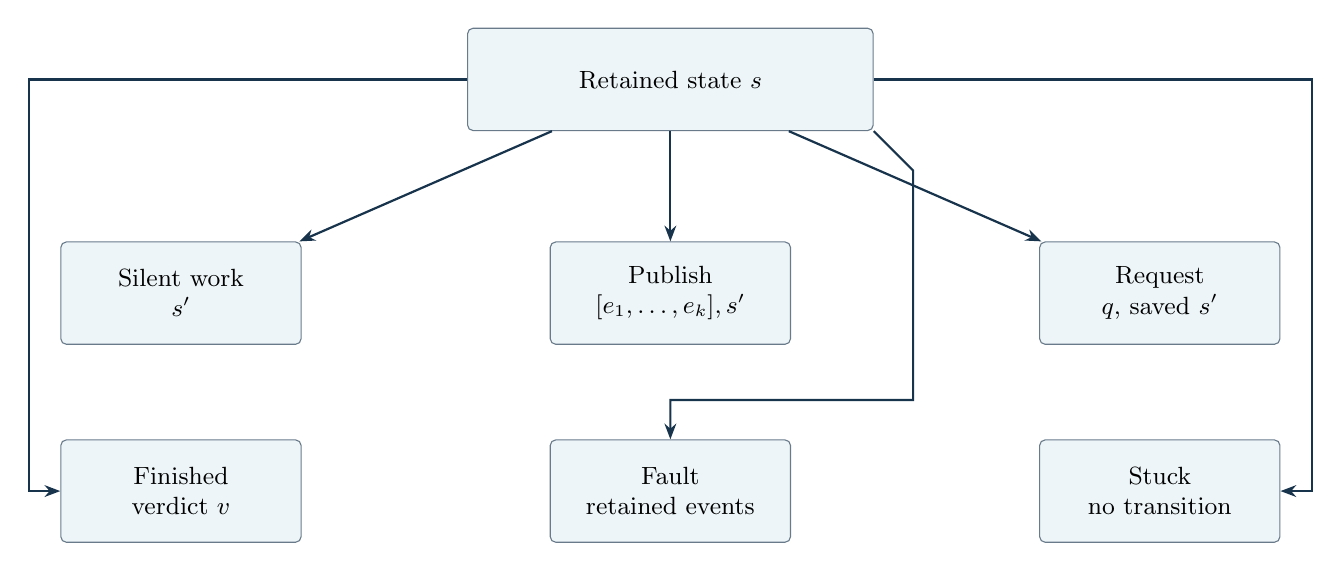
\begin{tikzpicture}
  \node[wide] (s) {Retained state $s$};
  \node[smallbox,below left=14mm and 21mm of s] (silent) {Silent work\\$s'$};
  \node[smallbox,below=14mm of s] (publish) {Publish\\$[e_1,\ldots,e_k],s'$};
  \node[smallbox,below right=14mm and 21mm of s] (call) {Request\\$q$, saved $s'$};
  \node[smallbox,below=12mm of silent] (final) {Finished\\verdict $v$};
  \node[smallbox,below=12mm of publish] (fault) {Fault\\retained events};
  \node[smallbox,below=12mm of call] (stuck) {Stuck\\no transition};
  \draw[arr] (s) -- (silent); \draw[arr] (s) -- (publish); \draw[arr] (s) -- (call);
  \draw[arr] (s.west) -- ++(-3mm,0) -| ([xshift=-4mm]final.west) -- (final.west);
  \draw[arr] (s.east) -- ++(3mm,0) -| ([xshift=4mm]stuck.east) -- (stuck.east);
  \draw[arr] (s.south east) -- ++(5mm,-5mm)
    |- ([yshift=5mm]fault.north) -- (fault.north);
\end{tikzpicture}
\end{center}
\diagramcaption{The arrows show possible transition or outcome kinds, not a sequence
that visits every box. Exhausting fuel retains a residual; it proves neither
completion nor divergence.}

A finite runner returns an ordered event list and an outcome. After fuel
exhaustion, running longer uses the saved residual and appends only the newly
produced events. A suspended request instead needs explicit response delivery;
extra fuel does not supply its answer. Finishing,
faults, suspension, stuckness and exhaustion remain distinct. Separate price
functions account for instructions, allocations or other declared resources.
An administrative rank excludes an infinite silent stretch when its hypotheses
hold; it does not assume the whole program terminates.

VM admission has two separate boundaries. A decoder admits a source compiler
image and retains its captured environment. The historical CAM, its
quotation/conditional extension and the graph CAM each prove the decoding,
loading and admitted-execution correspondence. At runtime, an independently
stated instruction table licenses the fetched operation in its current state.
Admitting the code for an open variable does not supply its missing environment;
an admitted image can therefore be stuck. Conversely, executable quotation code
can lie outside the historical compiler image. The graph loader admits compiled
recursion while rejecting arbitrary raw update instructions. Need's source-term
loader constructs its required source heap. Source-atom and C-program entries
retain their own language admission and realization obligations.

\subsection*{Three different choices in a stepper}

Semantic alternatives, redex selection within a branch, and scheduling between
branches have different contracts. For a pure snapshot, expanding one branch
$b$ can replace its frontier occurrence by the complete bag of its successors:
\[
  F'=(F-\{b\})+\mathsf{Succ}(b).
\]
Choosing which $b$ to expand need not discard any semantic alternative. Choosing
one successor and forgetting the others changes the computation. Occurrences
remain distinct even when their printed terms agree. Fairness is a separate
obligation for an infinite search; a finite pause establishes no exhaustive
answer collection.

Redex selection inside a branch must still follow its evaluation policy.
Call-time choice illustrates why unrestricted term rewriting is insufficient:
copies of one shared choice must not become independent choices. Let-rewriting
provides an explicit reduction presentation with soundness and completeness
against its call-time-choice semantics~\cite{LetRewriting}. Our branch-local
Need instance has its own independently stated judgments and adequacy laws;
that precedent does not establish native MeTTa adequacy automatically.

A source-level step also need not be one implementation instruction.
Clements, Flatt and Felleisen separately prove preservation by instrumentation
and reconstruction of the source reduction sequence~\cite{AlgebraicStepper}.
The corresponding obligation here is a constructed source/configuration map
and a productive block simulation. A debugger may expose that semantic view
without making all optimizer frames ordinary program observations.

Scheduling shared effects requires further evidence: commuting actions,
isolation, or an explicit serialization policy. The answer observer must also
be declared. Alpha-renaming of internal bindings cannot erase a string that
an ordinary operation has already produced from a variable's displayed name.
These distinctions prevent a scheduler-independence claim from silently
changing sharing, effects, or the language's observations.

\subsection*{The strongest useful form of correspondence}
A related source/native pair should reproduce the same selected occurrences,
with related residuals, at every relevant observation boundary. Native
administration may take several steps for one source step. A ranked block
simulation licenses that difference without erasing observable failures.
The backward direction establishes no invention; the forward direction
establishes that source behavior is realized. Cost bounds need an explicit
resource model in addition to behavioral correspondence.

\subsection*{A logical machine with replaceable backends}

The stable MeTTa machine is specified at the level of scoped evaluation
operations. Its configuration retains the term or task, binding constraints,
continuation, answer occurrences, observable world and required authority.
The selected language profile determines argument evaluation, rule freshening,
choice sharing, returned-value treatment and effects. A frame's address,
hash-table layout or symbol number belongs to a backend realization.
Logical object identity, freshness and ownership remain obligations wherever
the declared operations can observe them; changing addresses does not license
merging identities.

The representation boundary is a relation $R(b,s)$ between a backend state
$b$ and a logical configuration $s$. Several backend states may represent the
same configuration. At the declared observation boundaries, a logical step
$s\xrightarrow{e}s'$ must be realized by a finite backend block
$b\overset{e}{\Longrightarrow}b'$ with $R(b',s')$, and backend behavior must satisfy the
applicable reflection law. The block may contain internal administration;
productivity and endpoint laws prevent that administration from concealing
divergence, stuckness or faults. This is a behavioral obligation. A uniform
bound on the number or physical cost of backend instructions requires a
separate argument.

The existing event-machine interface now proves this finite-block connection
without a uniform cost premise. \name{Machine.run_related_of_one} derives
whole-prefix correspondence from local implementations of individual
inspections. Its resumption corollary retains the matched checkpoint and
appends only the suffix. Local implementations in both directions give equal
completed observations. Their outcomes retain faults, stuckness, requests and
related saved states; a separate corollary reflects unbounded execution within
the current interaction region. The local contracts compose through the
actual middle state. Costed stages retain their stronger resource law.

A checked control makes the difference concrete: each logical publication
has size-dependent internal work, with no single instruction bound for all
admitted states. Both directions preserve its duplicate publications and
completed observations; resumption appends the saved suffix, while restarting
repeats the prefix. Existing forward-only controls still demonstrate that
preservation alone cannot establish completion reflection. These generic laws
do not supply the missing local CeTTa, Rust or SWI implementation instances.

The local obligations concern loading, scoped query and binding operations,
invocation and return, host effects, retained control and observation.
Their constructed laws are inputs to the existing run-composition theorems.
Assuming the complete run correspondence as an implementation field would
not discharge those obligations. A new storage representation can replace
one backend instance while the language judgments and logical machine remain
unchanged. Representation differences can be hidden only when the declared
operations and future continuations respect the proposed relation; this
includes the identities correlating several uses of one unresolved variable.

The finite execution judgment also accepts relational local rules.
\name{DerivationSimulation} matches each independently justified source
inspection by a finite target derivation. Its \name{ExecutionReadout} maps
private event, verdict and request carriers to declared public observations;
the state relation retains the actual saved configurations.
An event contributes zero or more public records. Internal HE answer
publication can therefore remain private while ordered effects stay in the
public trace and the completed answer bag stays in the final verdict.
\name{transport} composes the local blocks along an arbitrary finite source
derivation, and \name{trans} composes realization stages through their shared
intermediate rules and readout. \name{resume} starts the suffix at the
already reached target residual and appends only its new events.
\name{completed_iff} requires a simulation in both directions. The control
\name{RelationalBlocks.no_backward} exhibits a forward realization whose
target additionally drops one duplicate answer on a separate branch.
Relabeling can hide private spellings while preserving both occurrences;
it does not justify coalescing them.
\name{CostSimulation.toDerivationSimulation} connects the deterministic
theory to this relational theory on the machines' step graphs. It requires
the separately constructed absent-transition law \name{MatchesStuck}.
The CAM graph/tree refinement and the independent fixed-C machine/codec
instantiate this adapter in both directions. It changes neither machine's
source language nor its observation contract. These finite transport laws alone imply
neither administrative productivity nor validation against a changed world.

The same relational laws now reach actual scheduled executions.
\name{EventCursor.advance_simulation} transports the shared cursor's result
to a finite target derivation, retaining its public history and the exact
source account. \name{resume_simulation} constructs the target prefix and
suffix at one reached intermediate configuration; it does not restart either
prefix. When both rules are executable, \name{advance_machines} compares
actual cursor results on both sides, with independently priced allowances.
The CAM graph/tree and fixed-C machine/data comparisons instantiate this law
in both directions. Their representation relations retain the caller stack
or the C memory, activations and service status. These scheduled comparisons
do not assert equality of physical costs or add a scheduling choice to the
language semantics. A branching-target control retains two equal public
occurrences through distinct private labels; no source scheduling allowance
can realize the target's extra completed branch that discards one occurrence.

Implementation evidence has its own scope. A formal proof about a memory
model, a source-fragment correspondence under ABI and service assumptions,
and an executable conformance test support different claims. In particular,
a model theorem conditional on a backend contract is not an unconditional
correctness theorem for the compiled evaluator. Physical helper proofs
strengthen an instance; they do not become definitions of MeTTa evaluation.
The independent fixed C-core development remains a separate substantial
instance of the common theory.

The same comparison framework also guides machine redesign. Explicit
continuations can replace hidden evaluator calls; one invocation dispatcher
can replace duplicated classification; a retained binding representation can
replace repeated reconstruction. These are machine refinements when the
specified observations are preserved. They earn efficiency claims only through
an appropriate cost comparison and measurements of the actual implementation.
A small change to the evaluation policy may instead yield a more coherent
language. Such a change is an explicitly compared semantic candidate, with
programs distinguishing the two policies and laws explaining the gain. It is
not evidence for equivalence under the old observation. The relevant choices
include fault versus ordinary failure, repeated evaluation versus ready values,
and who may inspect, advance or publish a retained computation. A licensed
transition and possession of authority to perform it remain separate judgments.
Execution determinism, answer cardinality and probabilistic meaning are
separate dimensions (Section~\ref{sec:contracts}). Focused graph holes and
changes of resolution follow in Sections~\ref{sec:holes} and~\ref{sec:zoom}.

\sources{\name{Mettapedia/Machines/MachineSubstrate.lean},
\name{Mettapedia/Machines/ProductiveCoreAdapters.lean},
\name{Mettapedia/GSLT/Distinction/ProductiveBlocks.lean},
\name{Mettapedia/GSLT/Distinction/SpanTransport.lean},
\name{Mettapedia/GSLT/Distinction/SimulationComposition.lean},
\name{Mettapedia/GSLT/Distinction/OrderedAdministration.lean}.}
\scope{These are common execution interfaces. They do not make the selected
logical kernels equal, or automatically prove a native evaluator refines them.}

\newpage
\section{CEK and Krivine: one syntax, different demands}

Both examples use de Bruijn lambda terms with natural-number literals.
The CEK-shaped machine implements left-to-right call by value. Its environment
contains values; its continuation first remembers an argument, then the
evaluated function. The Krivine-shaped machine uses call by name: its argument
stack contains closures whose evaluation is deferred.

\subsection*{CEK stepper}
For an application, evaluate the operator, evaluate the argument, and enter the
function's captured environment extended by the argument value.
\begin{center}
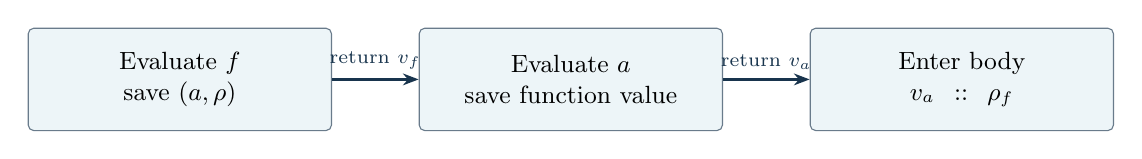
\begin{tikzpicture}
  \node[box] (f) {Evaluate $f$\\save $(a,\rho)$};
  \node[box,right=11mm of f] (a) {Evaluate $a$\\save function value};
  \node[box,right=11mm of a] (body) {Enter body\\$v_a::\rho_f$};
  \draw[arr] (f) -- node[hint,above]{return $v_f$} (a);
  \draw[arr] (a) -- node[hint,above]{return $v_a$} (body);
\end{tikzpicture}
\end{center}
\subsection*{Krivine stepper}
Push the argument closure, enter the operator, and bind the saved closure when
a lambda is reached. A variable lookup resumes its closure.
\begin{center}
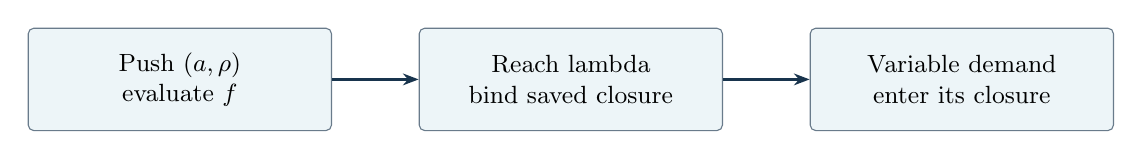
\begin{tikzpicture}
  \node[box] (save) {Push $(a,\rho)$\\evaluate $f$};
  \node[box,right=11mm of save] (lam) {Reach lambda\\bind saved closure};
  \node[box,right=11mm of lam] (use) {Variable demand\\enter its closure};
  \draw[arr] (save) -- (lam); \draw[arr] (lam) -- (use);
\end{tikzpicture}
\end{center}

The existing \name{CEK.eval_to_machine} and
\name{Krivine.eval_to_machine} theorems construct machine paths from successful
independent evaluator results, uniformly in the surrounding continuation.
The common adapters expose checked answer boundaries, finite traces, resumption
and computational accounts. This endpoint development does not mechanize the
entire CPS/defunctionalization derivation.

A discriminating term is $(\lambda x.\lambda y.x)\;7\;\Omega$.
Call by value evaluates the discarded divergent argument, so its evaluator
returns no answer at every finite fuel. Call by name reaches $7$ without
demanding that argument. This is a proved strategy difference, not an
implementation defect.

\sources{\name{Mettapedia/Machines/FunctionalCorrespondence.lean},
\name{Mettapedia/Machines/MachineSubstrate.lean},
\name{Mettapedia/Machines/ProductiveFunctionalMachines.lean}.}
\scope{Call by name does not memoize. Repeated demand may repeat work;
branch-local call by need requires the additional cell and cache laws below.}

\newpage
\section{The historical Categorical Abstract Machine}

The CAM follows Cousineau--Curien--Mauny's source strategy and instruction
tables~\cite{CAM}. One indexed source grammar contains variables, lambda,
application, pairs and projections, with literals and Boolean conditionals
enabled by its extension index. Source closures retain source bodies;
machine closures retain compiled instruction lists.

\begin{center}
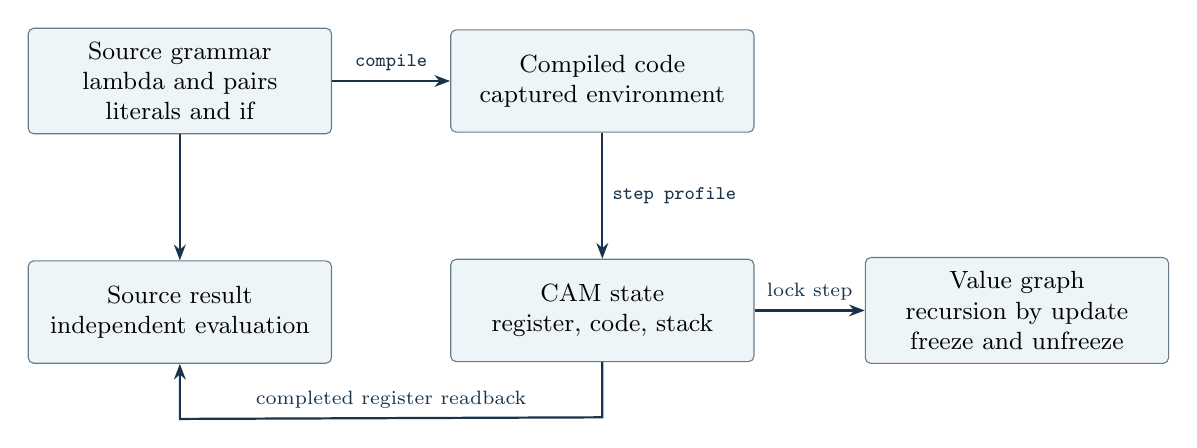
\begin{tikzpicture}
  \node[box] (source) {Source grammar\\lambda and pairs\\literals and if};
  \node[box,right=15mm of source] (code) {Compiled code\\captured environment};
  \node[box,below=16mm of source] (result) {Source result\\independent evaluation};
  \node[box,below=16mm of code] (state) {CAM state\\register, code, stack};
  \draw[arr] (source) -- node[hint,above]{\texttt{compile}} (code);
  \draw[arr] (source) -- (result);
  \draw[arr] (code) -- node[hint,right]{\texttt{step profile}} (state);
  \coordinate (sread) at ([yshift=-7mm]state.south);
  \coordinate (rread) at ([yshift=-7mm]result.south);
  \draw[arr] (state.south) -- (sread) --
    node[hint,above]{completed register readback} (rread) -- (result.south);
  \node[box,right=14mm of state] (graph) {Value graph\\recursion by update\\freeze and unfreeze};
  \draw[arr] (state) -- node[hint,above]{lock step} (graph);
\end{tikzpicture}
\end{center}
\diagramcaption{The tree machine and the value-graph machine share one instruction table.
On the tree machine's instructions they move in lock step; recursion and delay run
only on the graph.}

Application compiles to saving the environment, evaluating the operator,
restoring the environment, evaluating the argument, constructing their pair,
and applying. The actual state retains the register, remaining instructions and
stack throughout this work. The executable \name{step} agrees in both
directions with the independent \name{Transition} rules.

The shared compiler and code/value decoder have proved inverses on their
admitted images, including captured closure environments.
\name{evaluation_iff_execution} connects independent evaluation to completed
neutral-profile execution at both indices; completion requires empty code
and stack. A conditional evaluates its condition, restores the saved environment
and runs only the selected arm. A non-Boolean condition can be stuck.
\name{Lambda.proposition_3_2} connects historical scoped weak source reduction
to execution and readback at either syntax index, including literal and
conditional source terms and captured scoped environments. The strategy does
not reduce under a lambda.
Typed source formation constructs actual Cartesian closed morphisms;
\name{Typed.evaluation_iff_strict_execution} and the meaning theorems connect
the active instruction table to that interpretation.

The historical constant-free compiler remains the disabled-index specialization;
its no-quotation/no-branch laws and typed Cartesian-closed results keep that
scope. The enabled source uses the existing native quotation/branch instructions.

Recursion and delayed evaluation follow the paper's Sections~4 and~5 on a value
graph. Heap cells are couples, closures and frozen computations. Allocation
appends a cell; \name{wind} updates the second component of an existing couple,
as LISP's \name{rplacd} does. Recursion compiles as in the paper's Table~6 and
leaves the cyclic closure $c = C{:}(s,c)$ in the register. \name{freeze} builds a
frozen computation and \name{unfreeze} forces it at strict positions (Table~7);
forcing is by name. The module records two corrections to the published listing:
\name{unfa} and \name{unfb} rebuild the couple with exchanged components, and the
\name{letrec} code of Section~5 has a stray \name{swap}.

An independent big-step judgment covers recursion, frozen values and strict
primitives. \name{evaluation_iff_execution} relates it to completed execution
without assuming termination; executions keep the caller's code and stack and never
change existing cells. Heap words represent source values by finite derivations.
A cycle represents both a recursive value and its unfolding
(\name{Represents.not_functional}), so source syntax is not observable on the graph;
represented words agree with the depth-indexed unfoldings of their values, and
bisimilarity is agreement at every depth (\name{Represents.bisimilar_iff}).
\name{refinement} and \name{abstraction} are cost-one simulations between the tree
machine and the graph machine on the tree's instructions. Allocation keeps the heap
topologically ordered; \name{wind} breaks the order, and its cycle has no tree
unfolding (\name{windHeap_no_unfolding}). Controls run the paper's factorial and
lazy stream, a divergent loop, and stuck cases.

A memoizing variant uses the existing branch-local demand store. Each frozen
cell has its own allocation identity and immutable origin. Starting evaluation
records an owner; nested update frames retain the caller until the result can
be committed. Later forces read the completed cache without restarting its
producer. Separate allocations of equal source terms remain separate demands.

The independent source judgments \name{Need.Evaluation},
\name{Need.Invocation} and \name{Need.Force} use source constructors, an arena
and a demand store. They have no machine control or transition premise.
\name{Need.evaluation_iff_execution} proves both directions for complete values
and the entire retained world, including recursion, conditionals, cached hits
and nested updates. Its source-arena condition requires stored closure and
suspension bodies to be compiled source terms; the empty loader establishes
that condition directly. Active ownership blocks recursive demand. This is
explicit memoizing semantics, distinct from the historical by-name strategy.

\sources{\name{Mettapedia/Machines/CategoricalAbstractMachine.lean},
\name{Mettapedia/Machines/CategoricalAbstractMachineGraph.lean},
\name{Mettapedia/Machines/CategoricalAbstractMachineControls.lean}.}
\scope{Cartesian closure supplies typed meaning, not recursion or update; the graph
machine gives those their own operational laws. The extended readback and
memoizing correspondence are constructed. Logical instruction counts do not
by themselves establish physical performance or a native-code compiler.}

\newpage
\section{Branch-local Need: choose once, reuse in that branch}

The existing call-time-choice core separates value expressions from
computations. The distinction follows the call-time-choice separation between
shared demand and unrestricted rewriting~\cite{LetRewriting}. Its runtime
distinguishes a memoized implicit suspension,
a resampled implicit thunk, and explicitly quoted code. A cell retains its
original code and environment while its cache changes state.

\begin{center}
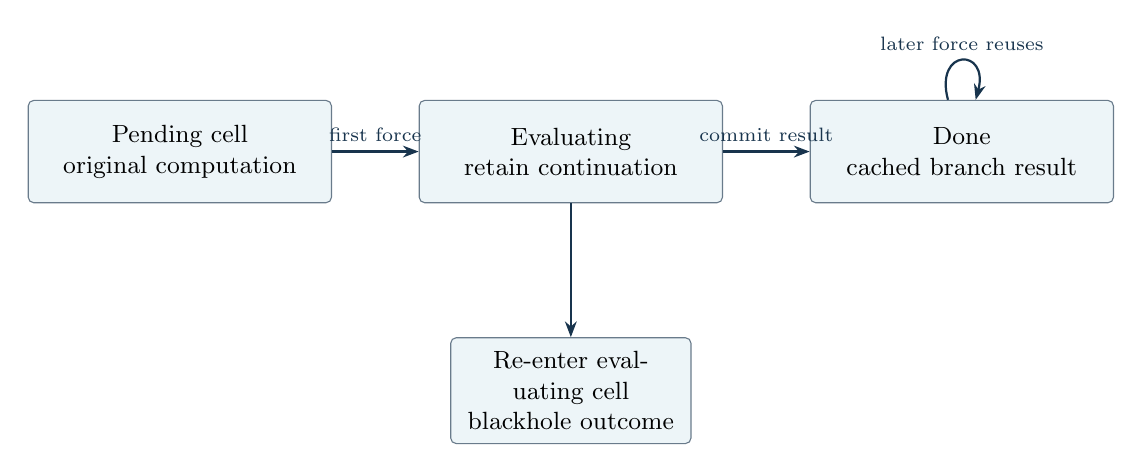
\begin{tikzpicture}
  \node[box] (pending) {Pending cell\\original computation};
  \node[box,right=11mm of pending] (running) {Evaluating\\retain continuation};
  \node[box,right=11mm of running] (done) {Done\\cached branch result};
  \draw[arr] (pending) -- node[hint,above]{first force} (running);
  \draw[arr] (running) -- node[hint,above]{commit result} (done);
  \draw[arr] (done) to[loop above,looseness=5]
    node[hint,above]{later force reuses} (done);
  \node[smallbox,below=17mm of running] (cycle) {Re-enter evaluating cell\\blackhole outcome};
  \draw[arr] (running) -- (cycle);
\end{tikzpicture}
\end{center}

\begin{center}
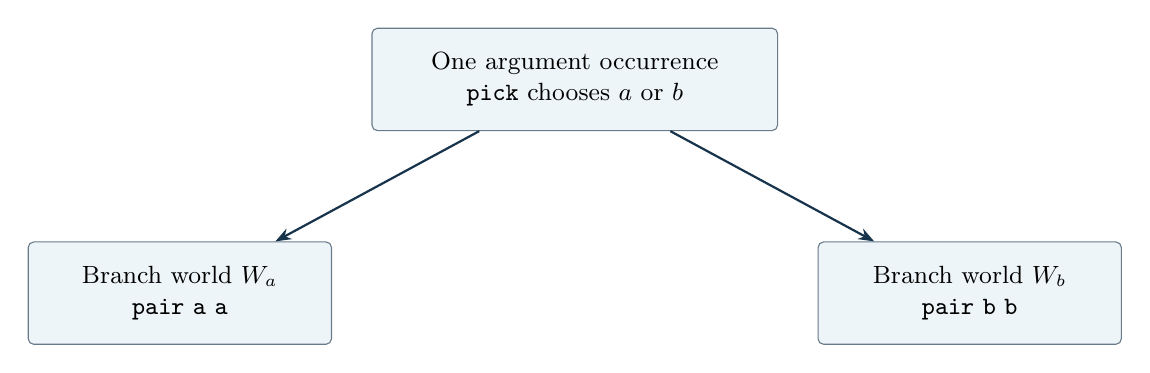
\begin{tikzpicture}
  \node[wide] (pick) {One argument occurrence\\\texttt{pick} chooses $a$ or $b$};
  \node[box,below left=14mm and 5mm of pick] (a) {Branch world $W_a$\\\texttt{pair a a}};
  \node[box,below right=14mm and 5mm of pick] (b) {Branch world $W_b$\\\texttt{pair b b}};
  \draw[arr] (pick) -- (a); \draw[arr] (pick) -- (b);
\end{tikzpicture}
\end{center}
\diagramcaption{Both uses share one chosen value in their own branch. A cache written
in $W_a$ does not become the cache of $W_b$. Separate argument occurrences can
still make independent choices.}

The natural semantics \name{Derives} is independently defined. The
\name{adequacy} and \name{observes_iff_halts} results connect it to the
unchanged branch-local Need machine in both directions, keeping the ordered
list of outcomes and duplicate occurrences. Failure and blackhole outcomes
are explicit. The strict-position theorem ensures primitives receive normal
forms under the modeled binding policies.

The finite weighted fragment is connected to these same machine runs.
\name{needChain_machine_adequacy} covers a finite ground producer, an arbitrary
finite chain of dependent producers and an arbitrary admitted final body.
Each intermediate producer may force its immediate predecessor repeatedly.
For sufficiently large frontier allowance, the actual frontier is completely
halted and each ground answer occurs exactly as often as the independently
defined weighted denotation requires. The relation also retains branch-local
heaps, cached choices and ordered effects. No conversion of cell identities
to ground values is used to obtain the counts.

Two machine-level controls distinguish the contracts. Forcing one duplicated
producer twice gives two shared occurrences; resampling it gives four.
Ignoring a failing producer succeeds under Need and fails under eager
execution. The allowance here bounds frontier unfolding, not total work.
The fragment does not admit arbitrary access to all earlier cells, and these
laws do not supply mutable-world validation or execution authority.

Quoted code is a value until explicit activation. Structural observation may
materialize an implicit pending cell under its original world and force rights;
it must not infer execution permission from a callable-looking written subtree.

\sources{\name{Mettapedia/Machines/BranchLocalNeed/CallTimeChoiceSpec.lean},
\name{Mettapedia/Machines/BranchLocalNeed/CallTimeChoiceBackward.lean},
\name{Mettapedia/Machines/BranchLocalNeed/CallTimeChoiceStrict.lean},
\name{Mettapedia/Machines/BranchLocalNeed/Weighted/StressAndCommitments.lean},
\name{Mettapedia/Machines/BranchLocalNeed/SharedContinuationInstance.lean}.}
\scope{This is source/model adequacy. Full native heap, producer/world identity,
resource retention and evaluator correspondence require their own joins.}

\newpage
\section{Refocusing: retain the route to the next redex}

A reduction evaluator repeatedly decomposes a term, contracts a redex, and
plugs the result back into its context. Refocusing keeps the context and searches
from the contractum, avoiding unnecessary reconstruction when the strategy's
laws justify it~\cite{Refocusing}.

\begin{center}
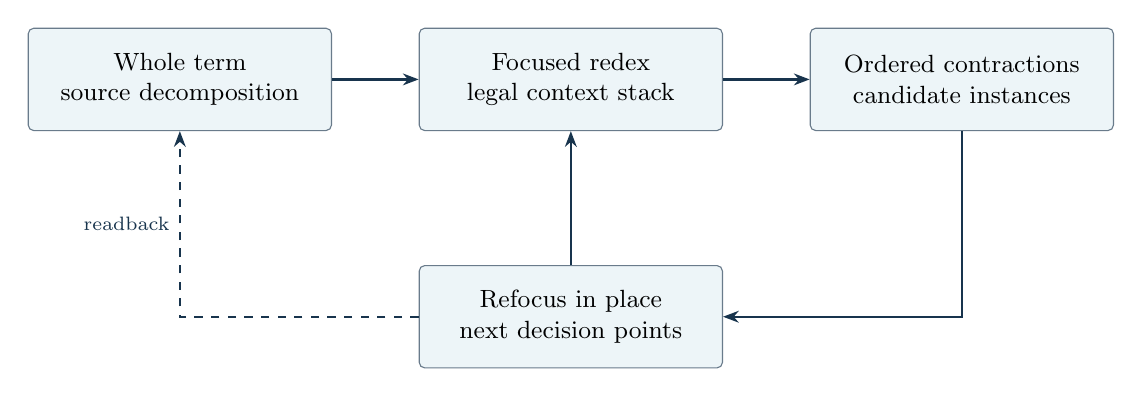
\begin{tikzpicture}
  \node[box] (whole) {Whole term\\source decomposition};
  \node[box,right=11mm of whole] (focus) {Focused redex\\legal context stack};
  \node[box,right=11mm of focus] (contract) {Ordered contractions\\candidate instances};
  \node[box,below=17mm of focus] (refocus) {Refocus in place\\next decision points};
  \draw[arr] (whole) -- (focus); \draw[arr] (focus) -- (contract);
  \draw[arr] (contract.south) |- (refocus.east);
  \draw[arr] (refocus) -- (focus);
  \draw[arr,dashed] (refocus.west) -| node[hint,near end,left]{readback} (whole.south);
\end{tikzpicture}
\end{center}

Frames are supplied by the evaluation strategy; their kinded stacks reuse
\name{Quiver.Path}. A structural syntax position alone does not authorize
evaluation. Traversal supplies local inspection and frame-resumption equations.
The branching strategy supplies candidates in order and ordered instantiations
for each candidate.

Inspection and rejected candidate attempts are administrative work, ranked by
\name{SearchCredits}. A focused computational step remains visible even if
its source and target terms are equal. A rejected candidate can be an empty
block; an observable fault or unmatched redex cannot be discarded on that basis.

\name{refocusingComplete} constructs reverse tracing from local
unique-decomposition laws. \name{blockSimulation}, \name{frontiers} and
\name{outcomes} preserve ordered alternatives, multiplicity and pending work.
\name{observable_stable} and \name{erasure_licensed} record the fault boundary.
\name{Authored.ruleScan_simulation} supplies an actual GSLT rule-scan instance.

\subsection*{Where generalization is still needed}
Several legal redex positions require an explicit position-selection policy.
The present unique-decomposition instance must not be silently treated as a
theorem about every parallel or nondeterministic traversal. Effectful attempts
also need a history model: erasing a rejected attempt is licensed only if its
observable commitments are accounted for.

\sources{\name{Mettapedia/Machines/Refocusing.lean},
\name{Mettapedia/Machines/RefocusingControls.lean},
\name{Mettapedia/OSLF/MeTTaIL/DerivedContexts.lean}.}
\scope{The authored rule scan is a real anchor. It does not yet establish the
full native evaluator's contextual traversal or administrative rank.}

\newpage
\section{HE and Prime: the retained representation boundary}

HE, PeTTa and declared Prime profiles are distinct language selections. A
common machine substrate can retain the selected package and its own state
without making those dialects interchangeable. Changing the selected
interpretation requires a justified crossing, not merely a new label.

The implementation boundary matters. LeaTTa is an auxiliary interpreter;
its correctness and conformance to HE are not acceptance conditions for
the CeTTa machine correspondence. A theorem about LeaTTa's instruction
worker establishes a property of that worker, even when its source judgment
is independently specified. It supplies no CeTTa transition map by itself.
HE semantic claims answer to the independent judgments and published
language contract. Rust HE and other engine runs supply separately labelled
conformance evidence; disagreements remain explicit. The realization target
is the retained driver's semantic component interfaces: selected
occurrences, binding readout, caller/alternative control, world operations and
publication. Concrete frame layouts and instruction phases belong to their
downstream representation examples.

The HE source and abstract-machine dependency graph excludes LeaTTa
implementation studies, including studies whose filenames do not name that
implementation. Binding models, finite matcher completeness, freshening and
valuation transport have their own mathematical owners. Neutral facts use
\name{Spec.Match.SolutionTheory}, \name{BindingComposition},
\name{MatchSizeTheory} and
\name{Spec.Bindings.ScopeObservation.ModelTransport}; they are not exported
through an interpreter-comparison namespace. The shared
\code{MeTTailCore.MeTTaSyntax.Atom} module owns the structural carrier in an
independent package. Both the HE mathematics and implementation clients
depend on that module. Every LeaTTa package module, including its former
\name{Core.Atom} owner, is excluded from the HE source and machine graph.
The shared leaf has no imports; the boundary check enforces this direction.
The independent HE freshener realizes the
alpha/freshness contract; comparisons with another implementation's
freshener remain downstream instances.

\begin{center}
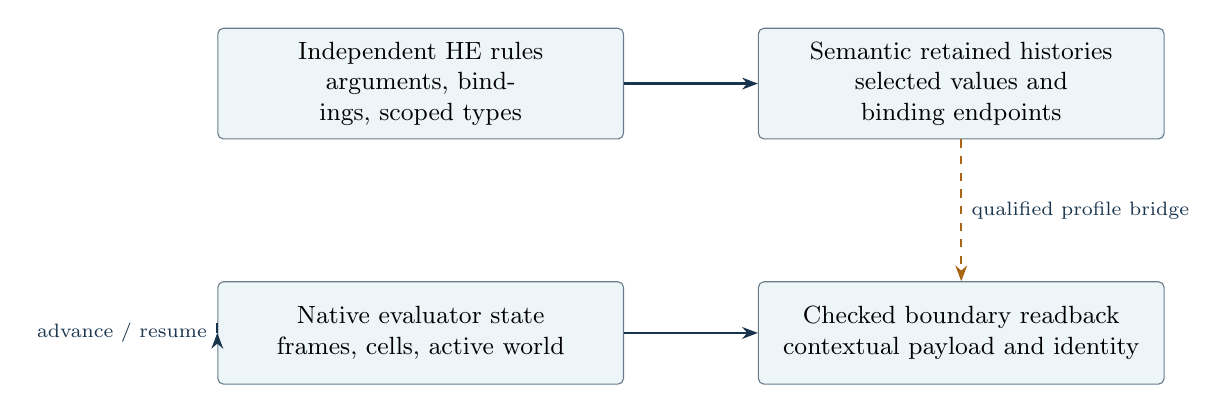
\begin{tikzpicture}
  \node[wide] (source) {Independent HE rules\\arguments, bindings, scoped types};
  \node[wide,right=17mm of source] (history) {Semantic retained histories\\selected values and binding endpoints};
  \node[wide,below=18mm of source] (native) {Native evaluator state\\frames, cells, active world};
  \node[wide,right=17mm of native] (payload) {Checked boundary readback\\contextual payload and identity};
  \draw[arr] (source) -- (history);
  \draw[arr] (native) -- (payload);
  \draw[arr,dashed,draw=amber] (history) -- node[hint,right]{qualified profile bridge} (payload);
  \draw[arr] (native.west) to[out=180,in=180,looseness=3]
    node[hint,left]{advance / resume} (native.west);
\end{tikzpicture}
\end{center}

The independent argument judgment constructs an ordered history of selected
values and exact intermediate bindings.
\name{RetainedArgumentSpecification.arguments_history_iff} gives both
directions at that semantic boundary. Leaf and nonleaf service packages
connect further parts of the independent evaluation.

Live scope is part of the evaluation judgment. A recursive equation call
freshens its private variables away from the arguments, current bindings and
saved caller context. This matters even for a single rule: an inner call to
\name{inc} must not reuse the outer call's private variable. The executable
evaluator, declarative relations and contextual step relation carry this
scope explicitly. Context replacement consequently requires the appropriate
agreement of live variable inventories.

Resource exhaustion is a separate observation from completed failure.
The checked recursive machine retains the pending task and requests further
resources when its evaluation depth or a supporting query is insufficient.
Its depth-coverage checks follow the actual recursive dependencies; a
successful check proves stability under every additional depth allowance.
A completed checked run also certifies the whole evaluator result at every
greater evaluation depth, for each of its six entry points and internal list
traversals. The proof increases the depths in every saved caller frame, not
only the currently selected task. Equal answers at two shallow depths would
not suffice: both can be empty while a deeper run returns a value.
For all six entry points this completed execution constructs the existing
evaluation certificate, including its eventual-stability witness and retained
live scope. It is still a theorem about this evaluator profile; its matching
and typing leaves do not disappear from the independent-language boundary.

Binding materialization now has a structural sufficient depth. A resolver
marks fresh assigned keys, and syntax traversal decreases the current atom's
height. The finite remaining-key set and the maximum stored value height give
a decreasing rank for both ordinary and equality-aware resolution, including
compound values and detected cycles. Control forms use this proved bound
instead of a fixed numerical cutoff. Cycle detection is a different operation:
the existing finite dependency analysis checks the complete graph of assigned
values and their equality classes. Its result is equivalent to the independent
absence-of-cycles judgment and can retain an explicit cycle witness. Every
stored assignment matters, including a value hidden by a later lookup entry.
Satisfiability together with nonvariable assignment payloads proves this
admission condition by strict descent of interpreted term size. Nonvariable
lookup results alone do not: a shadowed variable assignment is a counterexample.
The older finite list evaluator is still an approximation:
an empty list from that evaluator alone does not certify completed failure.

The service adapter uses this checked machine. Replenishment preserves its
selected alternatives, caller stack, world and already emitted results.
Completed checked executions refine the corresponding finite evaluator run;
the resource request is propagated through the C service caller. Thus a
shallow budget suspends a recursive service, while a sufficiently provisioned
three-call example returns the successive values $3$, $7$ and $12$.

The same checked execution has an actual data representation. Each advance
reads its supplied configuration and preserves every saved frame, published
occurrence and pending resource request. Reading after encoding is an
identity; malformed input is refused. The shared partial-reader adapter has
identity and composition laws and preserves the exact finite run, its
suspended residual, stuckness and unbounded exhaustion. Its logical step
account excludes the physical cost of encoding and decoding. In particular,
an encoded exhausted or suspended run cannot become an accepted empty result.

Application selection also retains history. A selected branch starts after the
preceding branches have advanced the state; its seed and entry state are
therefore part of the correspondence. The shared argument-fold laws retain
this chronological origin. A theorem about normalization from empty bindings
cannot replace a theorem about that reached environment. General conversion
soundness must supply normalization and binding invariants at the retained
endpoint; the concrete nested identity and constructor examples establish
those conditions directly. General normalization adequacy remains a separate
obligation.

The equation-query observation retains a physical row together with the same
raw rule, freshened pair, match, ambient merge and emitted work item.
The explicit-scope query is sound at this boundary and observationally complete
for any legal private freshening of that same row. A constructed permutation
fixes the query, incoming bindings and retained caller names; valuation
reindexing preserves the full output solution theory. Private binding records
need not have identical spellings, and this existence theorem does not count
semantic derivations. Separate laws for the actual HE continuation retain
the changed binding frame of each instantiated body beneath any saved caller
stack. Their finite realizations inherit completion, representation and exact
saved-residual resumption from one shared proof. The service adapter carries
each full value/binding occurrence into both its event log and endpoint reply;
structured and represented execution share that result. The typed application
continuation also retains those full results, including the actual
success-priority filtering. A typed duplicate-equation control returns both
changed frames to a saved caller through the real callback transitions.
The argument continuation now resumes each head's remaining arguments under
that head's selected frame. A second argument following two equation results
keeps both changed endpoints; restoring the common input frame preserves the
packet values and fails the full-result observation.
The same control law covers changed error and Empty results: it publishes
that occurrence without evaluating the pending argument suffix. Its independent
history records either the completed packet or the first failure and the
unexecuted suffix. A saved head-return frame needs only the residual children;
it does not replay the completed head. Duplicate rejected casts remain separate
occurrences, and the public success-priority judgment excludes successful
alternatives only when total rejection has independently been established.

The following query-item and materialized-entry laws additionally concern an
auxiliary minimal interpreter. They describe useful representation boundaries,
but do not identify that interpreter with Rust HE or construct a CeTTa step
map. Completing its instruction coverage is not a prerequisite for the native
correspondence.

The scoped-query completeness law additionally constructs the interpreter's
actual \name{queryOpItemsOfRule} work item and its \name{evalResult}
continuation, preserving the entire saved minimal stack. These work items
are already merged; the older HE equation task expects pre-merge candidates.
Bounded HE application now has a constructed observation law at every fuel.
The existing canonical native model promotes it to equality after actual
materialization, and to invocation congruence because \name{evalOp}
substitutes before dispatch. This does not license raw shape inspection of
unresolved syntax, or establish transport through every later typed RHS.
The actual query-item theorem uses the same materialization boundary to
identify its emitted continuation with the independently freshened source
result after substitution.

An independent normal finite presentation of the binding equations now supplies
the materialized source entry. Its one-pass result and the actual query value
agree up to renaming residual variables, by the existing principality theorem.
Exact function arity, the broader function-head test and embedded-instruction
classification are preserved separately. A raw head guard on this normal
source value constructs both the independent raw-completion judgment and the
actual finished query item. Function entries instead supply alpha-related
body witnesses. This applies at the existing query materialization boundary;
it does not authorize evaluating held operands or inserting substitution into
raw structural instructions. Transporting arbitrary unresolved source syntax
or executing every related body remains a further obligation.

Function completion preserves fuel, native state, pending alternatives,
saved callers and earlier results. Open \name{cons-atom}/\name{decons-atom}
steps and their \name{chain}/\name{return} bodies are constructed on both
sides. The finished chain handler materializes its raw result under the selected
output bindings; no fixed-result premise is needed by the general bridge.
A bound head becomes a symbol while two correlated free occurrences stay shared.
The actual complete driver suffix retains its pending queue and earlier results.
Materialized entry is a separate operation: raw primitives do not substitute.
A bound tail alias distinguishes those entries, and empty deconstruction
exposes an uncovered source fault.

Unify has sound and complete finite endpoints, including shared and reflexive
variables, success and refusal. Source and native merge orientations need
only agree on their complete solution theories. The actual candidate list
retains its occurrences; fallback syntax stays raw until materialization.

A caller-indexed terminal observer agrees with the actual function handler
after materialization, and its prefix law preserves faults and publication.
The nearest saved caller stays raw as the \name{NoReturn} subject; without a
caller, the terminal is blamed. The existing source judgments now retain that
caller and protect entered chain/function syntax in the query scope. This is
the full-syntax frame policy; Rust's placeholder frames require an adapter.
Malformed forms and the difference between core HE and extended
LeaTTa instruction classifiers delimit those auxiliary results. These
source judgments now materialize every finished function-body result before
classifying it as terminal or scheduling an exposed instruction. The independent
relation is generated by finite binding-equation presentation, exists exactly
for satisfiable frames, and agrees with the actual resolver up to residual
variable renaming. Controls expose both a return marker and a further
instruction through a bound variable. This corrects raw-syntax terminal
classification. The general body/typed-continuation correspondence is supplied
by the contextual atom/task completion theorems; the plain-Atom worker uses its
separately admitted recursive profile.

Equation producers now earn this materialization from their actual matched
output frame and retain the saved continuation. Native producers declare a
separate raw-or-materialized binding mode, independently of whether they have
completed interpretation. Raw delivery keeps the authored atom literally;
materialized delivery must supply its independent presentation. These policies
do not identify raw LeaTTa callbacks with Rust's post-merge materialization.

\subsection*{An invocation instance belongs to its saved configuration}

The independent direct type-lookup fragment collects declarations over a
multiset space, using \name{TypeOccurrencesRel}. A complete enumeration is
supplied by \name{TypeEnumeration}; its soundness, totality and uniqueness laws
keep every stored copy and choose one coherent enumeration per query.
\name{CompleteTypeQueryRel} separately describes admissible individual queries;
it is not an evaluator policy pooling all enumerations into one run.
\name{StorageTypesRel} and \name{storageTypeService} explicitly
name the older list-storage instance. The source does not prescribe that order.
\name{enumeratedTypeService} and \name{scopedEnumeratedTypeService} supply
alternative complete policies to the existing evaluation judgments.
\name{TypeCastBatchRel.complete_space_perm} preserves the full set of admitted
casts when storage is permuted. It does not assert that two fixed policies
choose the same successful type: \name{first_success_can_change_binding}
constructs actual source cast derivations with different type bindings.
\name{dropped_duplicate_not_complete} rejects a traversal that loses one copy.
Thus selection order is addressed before publication, rather than hidden by
quotienting only the final answer list.

A schematic declaration such as \code{(-> $t $t)} shares one variable across
its argument and return positions. Independent invocations receive distinct
instances. A caller that already binds \code{$t} to \code{Number} must still
be able to invoke the scheme at \code{Bool} through a fresh private variable.
\name{scopedTypes} protects the names of the complete retained configuration,
including the continuation and published prefix; declaration inspection remains
literal. \name{EquationFreshening.getAtomTypesScoped_scopedTypeLookup} connects
the actual query list to the independent scoped type service.

The applicability, coverage and first-success proofs now accept the actual
type query. \name{fresh_polymorphic_scoped_selection} constructs the same
changed binding in the worker and independent source scan.
\name{fresh_polymorphic_scoped_step} executes that checked transition while
preserving the saved stack and emitted prefix. The operator's selected
signature is explicit; this local theorem does not yet prove the complete
polymorphic application and return.
\name{scoped_polymorphic_annotation_prefix} additionally derives that selected
instance from the stored annotation and the actual expression checkpoint.
Its two checked transitions retain the fresh variable, changed binding and
saved context, with exact subsequent resumption. The shared equality-graph
laws establish that linking fresh private instances leaves every unrelated
ordered alias class unchanged, including its representative and value order.

The retained binding interface has a representation-independent constructor:
\name{ReadoutCertificate.of_normal_theory} turns a normal finite table with
exactly the source record's solution theory into one certified readout for
all future operands. A finite tuple of the complete binding support and
stored keys earns one model-fixed residual permutation; it is then extended
to all variables and atoms. \name{ReadoutCertificate.fresh_assignment}
extends this certificate by a fresh equation, including open values that
avoid its new name. The native \name{scoped_type_assignment_frame} preserves
older alias classes and constructs exact covered reads and pending-tuple
absorption under that extended table.
\name{scoped_polymorphic_annotation_frame} joins this construction to the
actual two-transition annotation prefix, with its saved continuation and
emitted answers. This is a reached-frame and prefix correspondence; the
later function, argument and return correspondence remains separate.

The subsequent
\name{scoped_polymorphic_function_entry_configuration_square} advances a
unary repeated-variable arrow scheme through the actual selection boundary.
It relates three checked worker transitions to one contextual function-entry
step, constructs the changed certified frame, and retains arbitrary related
caller stacks and prior occurrences. Its argument has one declared symbol
type, and entry readiness is explicit. The executed caller-alias control
reserves names in the saved caller and earlier publication, keeps the caller's
\code{Number} binding, and gives the fresh instance \code{Bool}. A held-value
reuse control separates that source policy from raw-worker reentry. These
are earned selection and activation laws; they do not establish recursive
application for arbitrary schematic signatures.

The quantifiers matter. A result table proved identical for every saved
stack under literal lookup cannot be reused unchanged when the stack affects
fresh names. The remaining scoped correspondence must follow the actual
configuration and its chosen instantiation witness. Other legal source alpha
spellings require a joint observation relation, rather than literal completeness
for the executable's deterministic name choice. Likewise, the per-result
\name{EvalRel} does not specify a completed answer bag: collection, multiplicity
and success-priority errors need independent occurrence and completion evidence.

Changing a constraint representation also changes possible alias
representatives. \name{BindingSourceAgreement.typeMatch_finite} constructs a
finite source match after changing the input store, preserving its complete
solution theory and variable support. The latter also preserves the complete
ordered family of mutually fresh type instances.
\name{typeCastBatch_scoped_finite} consequently keeps the first successful
candidate and every duplicate failure occurrence. These laws construct the
new source match and merge; they do not assume an evaluator correspondence.
\name{TypeMatchRel.output_agreement} also compares any two actual source
matches over equivalent incoming stores: their reached theories and support
agree. For a fixed functional type query,
\name{TypeCastBatchRel.output_agreement} preserves the first success and each
failure occurrence, and \name{joint_observation_eq} preserves the complete
ordered caller/value observation. The literal \name{StorageTypesRel} profile
discharges that query condition. Scoped queries permit different legal alpha
instances, so their witness alignment remains a separate obligation; they
are not assumed functional.
Ordinary future unification has a separate representation law.
\name{ReadoutCertificate.support_union_apply} preserves the incoming support
plus the variables of each operand. A source candidate succeeds exactly when
its new equation and the incoming constraints have a common finite model.
\name{UnifyCandidateRel.transport_certified_reads} therefore constructs the
counterpart operation on an equivalent certified store, without assuming a
second selected output. Both success and no-match are preserved.
\name{certifies_paired_pending} earns the two later readout certificates,
absorbs every earlier pending read and preserves the complete correlated
packet observation. Opposite alias representatives satisfy this law; a normal
but uncertified table can change success into failure. These are ordinary
constraint-operation laws, with annotated readiness and host services still
requiring their own correspondence.
The worker's \name{scoped_worker_symbol_cast_enabling_bridge} now consumes
that finite input-store cast and constructs the independent source batch,
contextual frames and local machine step under arbitrary saved callers and
prior publications. Its output relation retains the joint caller/value
observer on every public scope. It no longer assumes a source-side output
batch or supplied output-frame comparison. The primitive fold now derives
that batch from the executable cast and its complete candidate coverage.
\name{scoped_worker_symbol_cast_of_covered_selected_models} supplies this
instance for nonvariable input assignments when each selected raw output
has a finite model. A second constructor earns those models from coherent
input classes and loop-free selected outputs. The admission is substantive:
a covered raw merge can create a cycle even from a consistent, loop-free
input. Conversely, an exhausted covered candidate has no finite source
match. The compound-arrow control rejects its first candidate, selects the
second, and preserves both correlated caller aliases. These laws construct
source batches and joint output observations. The configuration-level
fresh-symbol and repeated-arrow squares additionally construct the annotated
output frame and retain its readout certificate, caller frames and earlier
publications. A continuous control rejects an earlier arrow, selects a fresh
polymorphic instance, performs the next argument cast, and returns through
the actual caller to publication and completion. Its published expression
is held, as the selected marking policy requires. A second continuous suffix
reaches a distinct fresh instance without resetting the first frame. These
controls do not establish general schematic application adequacy at arbitrary
arity or recursion depth.

The complementary \name{headsStopped_block} relates two worker
administrative transitions to one contextual stopped-head rule. It retains
the stopped occurrence and pending siblings without demanding arguments.
The executed discriminator separates \code{Empty} from the ordinary symbol
\code{Error}; an error expression has its own stopping rule. The continuing
head-to-argument and argument-to-caller laws compose with these retained
frames. General recursive composition must still earn the next readout and
entry-readiness premises rather than infer them from erased output equality.

Literal covered-read equality is stronger. On unifying \code{$a} with
\code{$b}, the maintained alias store reads \code{$a}, whereas the contextual
left-binding unifier reads \code{$b}. The formal control
\name{variable_match_has_no_literal_frame_transport} excludes that literal
relation for every output of this contextual operation. Nevertheless,
\name{variable_match_joint_public_readout} proves agreement of the actual
joint caller/return packet. The general retained comparison must preserve
this joint meaning, readiness and future operations; agreement of the
constraint theory alone is not that comparison. The negative
\name{wildcard_without_model_is_not_finite} also keeps wildcard acceptance
separate from consistency of the caller.

The cast correspondence therefore has two distinct conclusions.
\name{ScopedConfigurationRel.cast_selected_step} uses a certified canonical
presentation match for subsequent control; its payload and type-query policy
are parameters. \name{ScopedJointFrameRel.lift_finite_cast} instead lifts any
finite-model source cast to certified frames and preserves joint public answer
bags, including opposite open-alias representatives. It does not claim literal
control alignment. Re-presenting a constraint record retains its environment
and readout, so \name{Frame.represent} cannot create a missing canonical match.
For a fixed syntactic query, \name{scopedEnumerationTypeLookup_congr} preserves
lookup under equal protected-name sets and equivalent binding records. This
does not identify different subjects produced by subsequent materialization.

Frame-read stability and evaluation status are separate obligations.
\name{FrameUnassignedOn} permits open operands whose variables are absent
from the retained substitution's domain. Empty frames satisfy it for every
query. Certified materialization earns it again, so
\name{Frame.read_idempotent} preserves the entire annotated value, including
nested readiness marks. A pending sibling retains this property across a
cast only when the cast's new assignment keys avoid that sibling. The
\name{private_type_cast} law records the required write footprint explicitly;
fresh candidate names alone do not establish that footprint. For a private
type cast, \name{Frame.CastRenewRel.pending_reads} derives preservation from
the existing source freshness theorem: the incoming presentation and both
matched operands avoid the pending scope in their keys and value variables.
Annotated unification inherits this theorem through its proved erasure.
\name{InvocationSelectionRel.selected_fresh} earns whole-arrow and domain
freshness from the actual scoped selection. This is stronger than the
key-only condition needed for idempotent materialization; the two invariants
are not interchangeable.

The existing contextual machine therefore remains parameterized by reentry
policy. Reinterpretation admits a materialized value regardless of its
status; reuse retains the active-entry condition and may deliver a held
expression directly. The plain-atom worker realizes the reinterpreting
profile. \name{ScopedResultRel.materialized_entry_ready} constructs its next
entry obligation from an actual covered read, including open results.
Erasing marks does not justify identifying the worker with a reusing profile.
These local laws do not yet prove the complete recursive invariant across
all selected casts and saved callers.

\subsection*{Nested success priority is an observation boundary}

The location of publication is observable even in a closed, untyped example:
\begin{verbatim}
(= (mixed) Good)
(= (mixed) (Error Early Failed))
(= (later) (Error Later Failed))
!(Box (mixed) (later))
\end{verbatim}
The mixed child publishes \code{Good} and discards its error before its
caller resumes. The later child then fails. The checked retained machine,
under both invocation-type policies, finishes with only
\code{(Error Later Failed)}, agreeing with the tested Rust HE and CeTTa
profiles. Filtering only after the whole tuple can instead resurrect the
discarded early error. Priority therefore does not commute with resumption.

The existing raw mutual judgments propagate unfiltered child results.
\name{NestedPriorityControls.raw_parent_early} constructs such a derivation;
\name{outer_only_source_cannot_cover_checked_run} proves that their
outer-only \name{EvalRel} cannot characterize even the atom support of this
completed run. This diagnoses the formal source boundary, rather than a
disagreement between the engines. The upstream tuple and argument rules
call the published, filtered \code{metta} judgment recursively.

The independent \name{OrderedProtocol.Completion.SuccessPriorityRel} states publication
of a supplied finite batch. Its laws preserve duplicates, exact support and
representation changes, and descend through batch permutation. The stateful
traversal keeps effects already produced by discarded branches. The theorem
\name{successPriority_source_iff} identifies the actual worker filter's
entire occurrence list, and \name{completed_priority_retained_filter}
consumes its saved filter frame without changing the reached space, caller
stack or earlier publications. These are local laws: they do not establish
that a supplied batch exhausts a recursive source search. Source/machine
adequacy additionally requires completed child phases at every licensed
evaluation boundary. A prefix containing only errors remains incomplete.

The traversal law \name{OrderedStateFlatMapRel.split} exposes the actual
middle world at any cut of the source occurrences. Its converse is the
existing append law. \name{PublishedTraversalRel.simulate} lifts local child
refinements to ordered, completed publication under a relation between
worlds and an error-class-preserving result map. Neither the world relation
nor the result map prescribes a storage representation. Mapping equal
results does not merge their separate occurrences, and discarding a result
does not restore an earlier world.

The positive mutual family \name{Completed.AtomRel} supplies recursively
published finite child batches over contextual values and certified value
frames. Entry reads the actual reached environment before classifying delivery,
casting or interpretation. Tuple traversal keeps the child values, and each
selected physical equation completes its own body after contextual unification.
The complete caller batch is read before success-priority classification;
marking follows that classification.

Reentry, marking, rebuilding and type-match admissibility are explicit local policies. The unmarked
intermediate profile reinterprets expressions and marks none. The recursive
rules also support reuse of held values, retaining nested statuses and the
selected environments. Cast renewal either retains the whole frame or follows
the selected source type comparison. It does not replay the output binding
record to infer value provenance.
This finite-frame contract is stronger than unrestricted raw type matching.
For example, an incoming constraint $x=(y)$ can be individually consistent,
and a structural type match of $y$ against $(x)$ can independently produce
$y=(x)$. The bare merge admits their union, which has no finite-term model.
\name{cyclic_type_match} constructs this raw success, whereas
\name{cyclic_cast_has_no_contextual_lift} excludes any certified finite
activation for its result. This is a counterexample about the raw source
relation, not a claim about scoped engine execution.

\name{CastResultRel.lift_iff_models} characterizes the missing condition
exactly: a completed raw cast has a contextual lift if and only if each output
constraint record has a finite model. Its constructive direction lifts the
selected structural match through contextual unification, preserving the
original payload and each diagnostic occurrence. The finite-model guard
rejects every representation of the cyclic success; ordinary logical
unification therefore selects its failure branch. A positive wildcard cast
retains the same nonempty activation. A finite-type profile can enforce this
condition, or a scoped admission theorem can establish it for the eligible
uses. Neither repair follows from representative renaming alone. Rational
trees would require a different value/readout contract; no raw default or
runtime is silently changed here.
The completed cast relation now takes its matching policy independently of
the lookup policy. \name{TypeCastBatchRel.change_matching} and
\name{matching_iff} transport a complete cast when the matching relations
agree on the actual query. In particular,
\name{TypeMatchingPolicy.raw_finite_cast_iff} preserves the raw cast on the
domain where its candidates have finite models, including the first-success
decision and failure occurrences.

The explicit candidate \name{Policy.finiteTypes} changes only match
admissibility from the ready-value profile. The guard is tested during
candidate selection, not after committing to the first raw success.
\name{CastResultRel.lift_finite_batch} constructs every contextual frame
without a separate caller-supplied model premise, and
\name{AtomRel.finite_cast} constructs the corresponding full source phase.
\name{finite_cast_step} supplies its actual machine transition beneath any
saved continuation and prior publication prefix.
\name{TypeCastBatchRel.total} constructs a source cast from any complete
finite type query under an arbitrary matching policy.
\name{finite_cast_progress} combines this existence law with finite-frame
admission to construct a machine successor, without assuming a completed
cast or termination of the enclosing recursive evaluation.
With the candidate list $[(x),\%Undefined\%]$, incoming constraint $x=(y)$
and expected type $y$, the raw profile chooses the cyclic first candidate.
The finite profile rejects it and selects the later wildcard, retaining the
incoming frame. \name{finite_cast_phase} and \name{finite_fallback_run}
construct this source completion and its completed execution through the same
machine. The general adequacy theorem remains quantified over the policy;
no new continuation forms or control machine are introduced. This does not
establish conformance of the candidate to scoped HE or to any runtime.
\name{held_variable_phase} completes a held value obtained through a
nonempty certified environment under arbitrary demand. The control
\name{held_call_profile_separation} changes only reentry: the same held
call is delivered under reuse and reduced by the shared equations under
reinterpretation. Under reuse, held function-shaped data stays reusable;
function syntax selected for interpretation requires instruction execution.

The general laws exclude mixed published successes and errors, split caller
traversal without losing the suffix, and preserve equal error occurrences with
distinct contextual frames. Expression entry remains the read-only untyped
tuple/ordinary-equation profile. Declared typed-argument traversal is covered
below; typed-function selection and application, minimal bodies, host effects
and collection require their further constructors and correspondence.
\name{NestedPriorityControls.completed_scoped_source_matches_run}
constructs an independent contextual source batch for the example above and
supplies a contextual small-step run with the same erased atom list as the
retained scoped worker. The general source/control result below applies to
the declared core; this control does not establish general refinement of
the scoped worker.

\subsection*{A contextual small-step machine}

The existing recursive-control owners also contain the contextual phase
machine. Its configuration is
\[
  \langle S,\;C,\;K,\;O\rangle,
\]
where $S$ is the read-only space, $C$ is pending work, a returned batch or a
saved child context,
$K$ is a stack of first-order continuations, and $O$ is the ordered published
prefix. The eighteen work modes are atom, tuple, tuple branches, typed arguments,
argument branches, function, function branches, invocation traversal, caller
traversal, call, equation bodies, return, minimal execution, function-body
iteration, raw invocation, raw equation bodies, one boundary and boundary
traversal. Their operands retain contextual values,
certified activations and the source's explicit live/protected scopes.
Continuations close a phase, form a tuple, resume tuple branches or callers,
and append or prepend the retained occurrence batches. Typed argument frames
retain source values and declared demands and distinguish successful argument
packets from propagated failures.

The local transition relation has seventy-seven rules. Entry classification,
complete casting, static signature selection and equation queries, and contextual unification are primitive
premises. Recursive evaluation is work to be executed beneath a continuation.
Closing a phase reads its complete caller batch, applies success priority and
marks the selected values. Only a returned batch with an empty continuation
can be drained into $O$, one occurrence per step. The final observer accepts
only an exhausted return queue and empty continuation; an accepted observation
has no outgoing transition (\name{observed_final}).
This observer retains complete logical values and activations; public atom
and scoped-binding views are further declared projections.

\name{local_source_back} reconstructs independent source work across every
local transition. The mutual completeness proof follows the eighteen source
judgments under an arbitrary surrounding continuation. Together they give
\name{source_iff_finished} and \name{source_iff_observed} for every retained
configuration, including its already published prefix. In particular,
\name{loaded_source_iff_observed} proves
\[
 \mathsf{Completed.AtomRel}(S,a,T,M)
 \quad\Longleftrightarrow\quad
 \exists c.\;\mathsf{load}(S,a,T)\longrightarrow^{*}c
              \;\land\;\mathsf{observe}(c)=\mathsf{some}(M),
\]
with fresh input syntax, the empty certified activation and fixed declared
dispatch, lookup and policy parameters. No machine execution is used to
define the source judgment.

\name{RecursiveExecution.Contextual.Protocol.Rule} reads those actual machine
steps through the common finite execution judgment. Internal control steps,
one-occurrence publication and the final observer have separate rules;
stuckness is not successful empty completion. \name{steps_exhausted} and
\name{exhausted_steps} preserve both the reached configuration and the exact
new publication history. \name{source_iff_derivation} proves that independent
source completion agrees with protocol completion. The binding-changing
function/chain control executes through this adapter under arbitrary saved
callers and earlier publications. The generic finite-block composition can
therefore use the relational HE machine without determinizing its primitive
fresh-name choices. The declared worker and the maintained HE/PeTTa component
instances establish their local laws below. Resource grants and live-world
service protocols remain separately stated adapters rather than implicit host
operations.

The existing world machine also has a constructed common execution reading,
\name{RecursiveExecution.Contextual.Stateful.Protocol.Rule}. It retains the
actual world, context, continuation and publication history at each cut.
Its source-to-protocol correspondence reuses the independent stateful source
judgment, and its completed verdict includes the reached world. The declared
public observer pairs a world observation with the joint caller/value answer
bag. The world observation can retain the source's effect history; equal
answer bags alone do not establish world agreement.

The previously proved \name{RestoreRepresentation.step} supplies the local
law of an actual \name{DerivationSimulation} instance. Its common transport
theorem executes the nonidentity alias representation through two restored
occurrences, a prior publication and a live caller. Completion agrees in
both directions, with duplicate answer observations retained. The effectful
control additionally composes two native writes at the actual first-write
cut. A reset world is distinguished even with the same final answer bag.
These results connect locally completed host-operation contracts; executing
and authorizing an external service protocol remains a separate obligation.

One concrete service connection is supplied by
\name{RecursiveService.AuthorizedAppend.operation_refinement_square}.
The declared indexed-space append operation uses the existing store action's
safety and update judgments. The source and logical machine retain arbitrary
caller frames and prior publications, while the existing permission-checked
provider performs the append. Its first provider request reaches the updated
store and retains a return continuation. Resumption completes that return
with one charged write; restarting the primitive appends a second copy.
\name{source_completion_iff} also inverts the independent source instruction,
fixing the permission, complete reply and entire reached world. Revocation
before the operation instead retains the store and produces a service fault;
no completed source result, including an empty batch, is derivable. This is the existing
nonconsuming permission profile, not a new authority registry or a native
commit/arbitration proof. It supplies one local operation instance rather
than correctness of every host operation.

The retained service boundary is constructed in the same owner as
\name{AuthorizedAppend.Retained.operation_refinement}. Its recognizer follows
only the selected operational context chain. The returned site carries a
proof that the native instruction occurs at that licensed focus; an arbitrary
subtree containing the same syntax does not become executable. The inner
context identity selects the writer, while all enclosing context labels,
inner caller stacks, the root caller stack and earlier publications remain
retained. A local source-authorized world step corresponds to a service call,
one provider request, its reply, and reinstatement of the reached evaluator
configuration. These are four cursor/callback inspections, not a constant
bound on the provider's internal work.

The intermediate cut is an actual handled cursor packet. Its provider world
already contains the write, while the saved caller still contains the input
world. Resumption reads the packet's world and publishes only the reply;
it cannot issue the write again. Restarting the instruction in that world
instead produces two stored copies, as an executed negative control shows.
A refused operation returns a fault paired with its unchanged world and has
no completed source instruction derivation. A bare cancellation contains no
world, so the adapter does not infer one from the stale caller. The existing
callback composition and stuckness laws have constructed instances with a
three-inspection bound per closed callback transition. This is one declared
operation boundary under arbitrary retained operational contexts, not a
complete native dispatcher or an interleaving commit/arbitration theorem.

In the same namespace, \name{validated_resume_reached_cut} joins dependency
validation to an actual relational AM prefix. The saved
store is the store reached at the pause, including earlier own writes.
An explicit external update chain supplies the current store; validating the
selected reader's reached stamp proves its current source agrees. The
operation's right is checked in the current authority world. Successful
rebasing changes only that world, and the licensed suffix performs the one
pending write with the existing service protocol. Both caller stacks,
activation frame, context labels and all prior occurrences survive.
A stale dependency or revoked right instead returns the exact saved
configuration before any provider operation. Controls distinguish an
unrelated edit, a changed dependency and revocation; they also reject the
original pre-write stamp. This is a direct Contextual Stateful AM connection
for the declared append service, independent of the plain-atom worker and
its type-annotation admission. External rebasing is not an evaluator step,
and the theorem does not transport arbitrary evaluator actions across
arbitrary changes of world.

The composed interaction theorem now uses one state throughout rather than
conjoining unrelated Need, service and reply facts.  A \name{JoinedState}
contains the dependent Need machine, retained HE configuration and issued-return
registry.  Its first edge demands and claims the suspended Need cell, leaving it
at its unique evaluating owner before any effect.  Its second edge validates and
rebases the still-pending HE cut.  Its third edge executes the one-append service,
checks the same complete read stamp and exact parent/provider/payload handle, and
physically releases that row while moving the live HE field to the delivered
configuration.  Its fourth edge commits that exact delivered configuration to
the \name{NeedDependentService} cell indexed by the
same reader, argument and complete captured read stamp.  The resulting
\name{TransGen} path preserves the
saved stack, context and publication prefix.  The endpoint has no remaining
native service site; a copied old handle is refused as unissued; and later cell
demands are independent of the producer callback.  Stale stamps and denied
current operation rights refuse before registry release.  The separate finite weighted Need-chain theorem remains a
sharing/multiplicity result and is not presented as this service trajectory.

\name{retained_prefix} keeps the exact earlier values and activations at every
later cut. \name{held_entry_exact} prevents a completed reuse from replacing
the held result; \name{completed_atom_no_mixed_errors} excludes mixed final
successes and errors. A nonempty-environment control runs below any saved
continuation without changing earlier publications, and its negative control
rejects a newly computed replacement. The reentry discriminator now supplies
both source completions and both corresponding machine paths.

The machine inhabits the common reduction-span interface with its actual
transition endpoints. Primitive fresh-instance choices remain relational;
their concrete selection and implementation comparison require realization
laws. This is a finite-completion theorem for the declared read-only core and
its typed invocation and minimal phases.
Finite completion does not determine when successes may become observable
during an unfinished search. Grounded host execution, captured binding
collections, effects,
answer-prefix productivity, full source progress/divergence, answer-origin
readout and the general scoped-worker/native comparison remain separate
coverage obligations.

\subsection*{Typed arguments retain their declared demands}

\name{ArgumentsRel} pairs each source value with its declared expected type.
Each child runs through \name{AtomRel}, with the remaining source values and
demands kept live. \name{ArgumentBranchesRel} processes each returned occurrence
under its actual reached frame before proceeding to its siblings. A changed
error or \code{Empty} stops that occurrence's remaining argument requests;
an unchanged literal error is argument data. These are different evaluation
contexts from ordinary tuple construction.

Success data must be distinguished from a propagated failure. The declared
HE encoding is \code{(Ok (arguments ...))}. The contextual value codec retains
whole children and its erasure agrees with the existing atom codec
(\name{unpackArguments_erases}). The protocol invariant
\name{ArgumentsRel.packet_or_error} admits only successful packets or
propagated failures, including when the argument payload begins with
\code{Error}. A concrete runtime may realize this logical boundary with its
own result representation; the theorem does not prescribe a C layout.

The two argument continuations resume the remaining occurrence traversal or
prepend a selected whole value to each completed tail packet. They reuse
the machine's existing append/prepend control. \name{arguments_complete} and
\name{argument_branches_complete}, together with the extended
\name{local_source_back}, join both source families to the general retained
configuration correspondence. Recursive child evaluation is explicit pending
work, not an argument-evaluator callback.

\name{raw_arguments_exact} preserves arbitrary open values and nested
statuses under raw \code{Atom} demands in the empty activation;
\name{raw_arguments_cannot_reinterpret} rejects a changed completed packet.
Nonempty-frame controls propagate an error read through a bound variable
without evaluating that occurrence's later requests. The binding-change
control starts with $x=y$, casts the first argument to obtain $y=T$, and
reads the second argument $x$ as $T$. Its reached frame certificate is earned
by actual contextual unification. The complete run and its variant beneath
arbitrary saved continuations preserve the frame and earlier publications,
for every declared policy. These laws are consumed by typed function assembly.

The scoped worker comparison separately earns the read at publication.
\name{ScopedResultRel.materialized_readResult} relates the native value
$b.\mathsf{applyFull}(v,d)$ to the contextual annotated read, using the
covered native read and both materialization laws. It does not assume that
the read is the original syntax. Its stable specialization and complete-list
version feed the actual filter/publication square without dropping repeated
occurrences. None of these erased-read equalities establishes active status.

Argument entry also retains the variables in every remaining value and
demand. The contextual request inventory and the worker's grouped values and
types need not be the same list; their protected-name support agrees.
\name{argsCons_step} consumes that agreement at arbitrary arity. The stopped
changed-error branch is a finite block of two worker steps and one contextual
step, retaining the skipped requests' surrounding caller and prior output.

A symbolic execution family composes these operations. From a returned head,
it casts a first symbol against a fresh binding variable, evaluates an
arbitrary finite tail of admitted raw symbols, assembles the application and
publishes it to the saved caller. A tail of length $n$ requires $8n+16$ silent
worker steps. The reached frame and the contextual held publication remain
related beneath arbitrary related saved callers and prior output. This is
the explicit \name{finiteTypes} candidate: reuse, successful marking and
preserved rebuilding remain unchanged. An executed three-argument instance
reaches completion; a separate two-occurrence publication step retains both
equal inputs. A bound-held-operand control earns the materialized erasure on
both sides but refutes active-entry admission solely by its held status.
\scope{The family starts at prepared head return and its tail consists of raw
symbols. It does not establish general recursive argument evaluation, typed
return, minimal-body adequacy or whole scoped-worker refinement.}

\subsection*{Typed invocation separates selection from recursive work}

\name{InvocationScanRel} describes a complete ordered signature scan. For
each arrow, \name{ApplicationChecksRel} checks every argument-type occurrence
under every incoming logical frame, then checks the return demand. A type
occurrence either supplies the primitive contextual constraint renewal or
has a negative match witness. Repeated declarations remain repeated
occurrences. A nonempty applicability batch selects that arrow and discards
earlier diagnostics; exhaustion retains all failed blocks and whether tuple
fallback is eligible. The scope-aware lookup is a parameter of this finite
operation. It contains no call to recursive language evaluation.

\name{ApplicationChecksRel.source_member} projects every accepted frame to
the existing independent \name{ApplicationSuccessRel}. The contextual
constraint renewal is constructed from a selected finite type match
(\name{Frame.TypeRenewRel.of_modelled_match}); finite matching makes each
single comparison total. This is not termination of recursive evaluation or
an equivalence with every presentation of the historical raw constraint
model. The latter's finite-model obstruction and the explicitly distinct
matching policies remain as stated below.

The selected batch enters \name{InvocationsRel}. Each occurrence evaluates
its head at the selected arrow, evaluates its arguments at their declared
demands, and passes the assembled application through the selected return
gate before advancing the next occurrence. An \code{Expression} return
changes the call demand to \code{\%Undefined\%}, following the declared
interpretation rule. Function head failures skip their pending argument
requests. Tuple fallback appends its saved diagnostic block before the
ordinary completed publication boundary.

Three new work modes and three continuation forms expose this work in the
same retained machine. \name{function_complete},
\name{function_branches_complete} and \name{invocations_complete} extend
both directions of the general retained-configuration correspondence.
The duplicate-type control traverses selection, head casting, raw argument
delivery, call and publication and retains both answer occurrences. Its
saved-stack variant retains prior work; a separate wrong-arity control
completes with its diagnostic. The negative
\name{duplicated_raw_type_occurrence_not_dropped} excludes deleting a type
copy. Nonempty-frame controls cover head failure and binding changes through
function assembly. These are source/AM results for the declared finite core;
the full scoped-worker comparison, grounded hosts, effects and collection
still require their separate joins.

\subsection*{Minimal bodies and saved contexts}

\name{MinimalRel} separates ordinary data from an explicit invocation.
Its evaluation rules use \code{eval} and \code{evalc}; continuation and
matching use \code{chain} and \code{unify}. The latter includes the declared
diagnostic for malformed arity. Structural rules use \code{cons-atom} and
\code{decons-atom}. Other rules execute a \code{function}, enter full
\code{metta} evaluation or read \code{context-space}.

\name{InvocationRel} consumes complete equation frontiers, retains one work
item per stored copy, and completes an
authored function wrapper once. Ordinary producer data stays raw. The typed
return gate subsequently decides its use through the existing entry policy.

\name{BodyRel} runs minimal work and reads its reached frame before checking
for another instruction. Five licensed boundaries share one ordered
\name{BoundaryBatchRel}: local chain substitution, body resumption, function
completion, producer completion and typed return. A local chain operand is
substituted into the template without a caller-binding write.
The substitution erasure law \name{substituteBinder_erase} agrees with the
existing independent \name{Minimal.substituteName}. Contextual unification
also projects to the independent \name{CoreStepRel}; the bridge is
\name{completed_contextual_unify_step}.

The source families index the context space, so recursive children may use
another space. A control \code{context}\,$(S',C',K')$ retains that child's
actual work and stack. \name{contextStep} lifts one child transition and
\name{contextReturn} returns its completed batch. The outer space, stack and
published prefix remain saved. Neither rule calls a recursive evaluator.
The additional six mutual completeness proofs and \name{local_source_back}
extend the same retained-configuration correspondence to these modes.

\name{immediate_function_exact} proves that a raw function return transfers
an arbitrary payload once, preserving open syntax and nested readiness;
\name{immediate_function_cannot_reinterpret} is its negative machine control.
The binding-changing control begins at $x=y$, unifies $y=T$ while yielding
$B$, substitutes the chain-local $x$ into \code{(return \$x)}, and returns
$B$ while the caller still reads $x=T$. The boundary's exactness law excludes
writing that local selection into the caller frame. A separate control keeps
the saved caller as the \code{NoReturn} diagnostic subject.

\name{evalc_saves_child} exhibits the actual paused child configuration;
\name{evalc_resumes_child} continues from it and reads the child context,
preserving arbitrary outer continuations and earlier publications.
\name{metta_raw_child_retains_stack} exercises complete full-evaluation child
delivery under an \code{Atom} demand. These results concern read-only
contexts. Grounded hosts, \code{call-native}, captured snapshots for
\code{collapse-bind}/\code{superpose-bind}, world effects and their native
realizations remain separate coverage obligations.

\subsection*{Evaluation status is an entry policy}

An occurrence which requires interpretation differs from a value ready for
delivery, even when both print as the same expression.
\name{Entry.Rel} separates delivery, type casting and expression
interpretation. Its classification is total and functional without assuming
that interpretation terminates. The \code{reuse} policy delivers held
expressions; \code{reinterpret} enters them again. Fresh entries have the
same classification under both policies. The theorem
\name{erasing_status_cannot_classify} excludes an atom-only dispatcher for
these two occurrence states.

Publication has a separate named policy: mark successful expressions, mark
only unchanged successful expressions, or retain unmarked results.
\name{publish_readout} preserves the entire occurrence list and binding
frames, and \name{publish_priority} transports success-priority
classification. This is not observational equivalence of later reentry:
the status deliberately determines whether later computation occurs. The
entry view specifies neither a storage bit nor a nested-value representation.
The contextual values below retain child statuses. \name{AtomRel.delivery_exact}
connects delivery after an actual frame read to the recursive source family
under every declared policy.

\subsection*{Substitution must retain contextual values}

\name{Entry.Value} records the status of every expression occurrence.
Its finite environments retain whole values at variable lookup. Erasing the
statuses commutes with simultaneous substitution
(\name{erase_substitute}) and with the existing finite-table readout
(\name{erase_substitute_environment}). One certificate for that table earns
\name{selected_materialization} in the existing binding frame.
\name{selected_held_variable_entry} additionally delivers a stored held
expression under every demand, retaining its nested statuses.

Constraint readout alone does not determine readiness. Two nonempty
environments can have the same certified erased table and different statuses
for the same variable
(\name{constraint_certificate_does_not_determine_status}). A contextual
realization must retain that additional information. Scope renaming preserves
statuses; inverse renaming restores the entire value
(\name{rename_cancel}).

The constraint record itself can change without choosing a new annotated
readout. \name{Frame.represent} retains the exact environment and constructs
its new certificate from complete constraint-model agreement.
\name{represent_read} preserves the whole annotated value under every policy;
the identity and composition laws make successive record changes coherent.
Full support agreement preserves the invocation's protected names as a set,
without requiring equal record order. A reversed equality edge and a
variable-valued assignment supply a nonidentity example. The separate
\name{constraint_agreement_alone_does_not_preserve_readiness} control rules
out replacing the retained environment by an arbitrary model-equivalent one.

Rebuilding exposes a distinct policy choice. The \code{preserve} policy keeps
data ready through substitution and satisfies ordinary environment fusion
(\name{preserve_compose}, \name{preserve_fuse}). The
\code{reopenChanged} policy reactivates a parent whenever its substituted
syntax changes. Swapping $x$ with $y$ twice in a held expression restores the
printed syntax but leaves the expression active. Fusing the swaps first
leaves it held (\name{reopen_composition_separation}). Thus syntax-level
substitution fusion does not imply contextual-value fusion for that policy.
This statement concerns the declared rebuilding rule; a dialect comparison
requires its own source contract.

Retaining the pending substitution sequence preserves intermediate changes.
\name{substituteAll_append} proves the prefix/residual law for either policy,
using the reached value at the cut. These operations manipulate semantic
values and environments; they neither evaluate language programs nor select
a backend representation.

Ordinary unification transfers these contextual values through assignments.
\name{erase_bind} projects each update to the existing finite-presentation
operation. \name{UnifyRel.erases} and \name{UnifyRel.lift} prove both
directions: annotations neither add nor remove successful ordinary matches.
The matcher compares syntax; readiness is not another equality constraint.
Each sibling uses the environment reached by its predecessor.

\name{UnifyRel.of_source_candidate} constructs a contextual trace and
certified reached readout for every surviving source candidate, including
open operands and incoming aliases. \name{contextual_unify_step} composes
this readout with the existing minimal-instruction rule and materializes its
continuation from the actual reached values. For a completed equation
frontier, \name{UnifyRel.equation_frontier} pairs every physical work item
with such a trace, retaining source order and separate occurrences.

The open-alias control starts with $x=y$, then binds $y$ to a held value
containing a free $z$ and a nested held child. Repeated uses of $x$ and $y$
retain that whole value. Filling $z$ later gives the same syntax under both
rebuilding policies, with readiness following the chosen policy. Distinct
symbols remain incompatible. These are source binding and materialization
laws used by the completed recursive source family and contextual control
machine. The core's completed source/control correspondence is proved above;
the further construct coverage and concrete realization joins remain.

\subsection*{Complete equation selection precedes body evaluation}

\name{EquationFrontierRel} supplies independent finite coverage for one
equation query. Every physical row is classified as a non-equation, an
equation with no viable fresh instance, or one selected principal constraint
theory. Equal equations stored at different positions remain separate
occurrences. Different proofs or equivalent records of one unifier do not
add alternatives. This is the equality-grounded matching profile; custom
grounded matchers that branch require their own occurrence contract.

The existence theorem \name{equationFrontier_exists} classifies every row
of any finite space, including with alias-bearing callers. It does not run
an evaluator or assume termination of an equation body. A negative row
certificate covers every legal alpha variant, rather than merely one
chosen spelling. \name{row_miss_of_instance} earns this universal coverage
from the absence of a unifier for one legal instance. The general
\name{occurrence_alpha_transport_logical} proves the required change of
instance by logical conjunction, without the older restriction excluding
variable-valued caller assignments.

The frontier laws prove both source soundness and coverage, distinct
physical origins, and invariant occurrence counts. The stronger
\name{frontier_covers_readout} also preserves the whole binding solution
theory and RHS observation under one permutation fixing every caller-visible
name. In particular, a name occurring only inside the value of a caller
alias is protected. A completed empty frontier is equivalent to absence of
every source query candidate. For an ordinary call this earns unchanged
query restoration, including its complete binding frame.

The actual binding-machine matcher and merge each return at most one
candidate in this profile. This bound alone says nothing about exhaustion:
it also holds at depth zero. The retained-machine controls compare a
four-row source frontier containing two equal equation copies with its
actual query, reject the empty truncated helper result as source completion,
and prove that the checked machine preserves the query as pending work.
General query refinement and recursively completed child evaluation remain
separate obligations; selecting a raw RHS does not evaluate it.

Unification has a stronger completed primitive join.
\name{covered_unifyReadouts_iff_source} proves that the actual covered
match/reconciliation search has a surviving result exactly when
\name{UnifyCandidateRel} admits a satisfiable conjunction. The caller may
contain bare aliases. The reverse direction constructs a finite semantic
size bound, earns actual matching and merging witnesses, and transports
them back to the covered depth using stability. It assumes neither a desired
result record nor whole-evaluator correctness.
Consequently \name{covered_unify_empty_iff} earns the source failure
judgment from completed search. The retained primitive derivation now uses
this theorem instead of requiring a separate source-absence premise, and
also covers rejection after a structural match succeeds. Its soundness
transports failure through either admitted binding observer; its execution
law keeps surrounding callers and earlier emissions. The positive alias,
post-merge failure and truncated-search controls distinguish these cases.

The whole query has a completed negative connection as well.
\name{source_occurrence_reaches_covered_query} transports any viable source
occurrence to the retained fresh instance and constructs a surviving actual
query item. It uses checked query and caller-merge coverage, without closedness
or alias normalization assumptions. Conversely, each actual prepared item
constructs an independent physical source occurrence and its readout.
The theorem \name{covered_query_empty_iff_source_frontier} combines these
directions: under the checked local query, merge and readout bounds, an empty
actual query is equivalent to an independently covered empty source frontier.
The frontier accounts for all stored rows and legal fresh variants; the
runtime's empty list is not its definition. A structural hit rejected by the
caller supplies the post-merge negative control. This settles this query's
absence boundary, not nonempty recursive answer multiplicity or body
termination.

\subsection*{A continuation slot is distinct from its binding environment}

The distinction has an executable counterexample:
\begin{verbatim}
!(function (chain (unify $x A B refused) $x (return $x)))
\end{verbatim}
Rust HE returns \code{B}. An earlier CeTTa image returned \code{A}, although
renaming the chain destination to \code{$y} produced \code{B}. The child
unification constrains \code{$x} to \code{A} and selects the branch
\code{B}; these are different pieces of information. Chain substitutes the
selected value into its saved template and carries the child's bindings
separately. Applying those bindings to the template first erases the slot.
For $\beta(x)=A$, the two operations need not commute:
\[
  [x:=B](\beta(x))=A \qquad\ne\qquad
  \beta([x:=B](x))=B.
\]
The repaired instruction path retains literal instruction operands and
performs the selected substitution before entering the continuation with
its reached environment. This also protects a nested instruction's future
destination from premature substitution. It does not turn minimal chain's
structural substitution into capture-avoiding lambda substitution: replacing
a slot can also replace the same name inside a nested instruction's syntax.
Each language profile must state the operation it actually provides.

Raw instruction shape checks expose another boundary. A variable constrained
to an expression is still a variable at a raw \code{cons-atom} or
\code{decons-atom} operand; substitution is licensed at the instruction's
specified boundary, rather than inserted before every shape test. For
\code{unify}, success requires a surviving match and merge. A match whose
merge conflicts with the incoming bindings selects the failure branch with
the original environment, rather than silently losing that occurrence.

The runtime qualification compares these cases with Rust HE across the
declared HE profiles and both canonical and fallback execution paths. Nested collection
additionally preserves captured bindings, repeated equal occurrences and
one committed effect across every scheduler pause. The implementations can
enumerate the same completed multiset in different orders; exact resumption
continues to preserve each implementation's own chronology. These are local
instruction and runtime results, not the complete native/source simulation.

\subsection*{A raw rewrite result still has a return continuation}

The root rewrite relation and the public evaluator observe different
boundaries. For example:
\begin{verbatim}
(= (freeze $x) NotReducible)
!(freeze (+ 1 2))
\end{verbatim}
Rust HE returns \code{(freeze 3)}. The argument has already been evaluated;
the returned protocol symbol asks the owning invocation to retain that
assembled call. An earlier CeTTa image instead published
\code{NotReducible}; an intermediate repair restored the unevaluated
\code{(freeze (+ 1 2))}. Neither observation implements that return rule.
The independent source relation also lacked this stage on its successful
equation and emitted-grounded branches. A checked counterexample exposed
the source defect independently of the native implementation.

Let $a$ be the assembled invocation, $v$ its raw result, $D$ its selected
return demand and $\beta$ its reached bindings. The ordinary return
judgment has three cases:
\[
 \operatorname{return}_{D}(a,v,\beta)=
 \begin{cases}
   [(a,\beta)] & v=\mathsf{NotReducible},\\
   [(v,\beta)] & v\text{ is Empty or an error},\\
   \operatorname{eval}_{D}(v,\beta) & \text{otherwise}.
 \end{cases}
\]
This is an intermediate judgment; the public observation still performs
its own filtering. The repaired source rules and retained worker both
represent this continuation explicitly. The invocation, bindings and
demand survive a scheduler pause. Restoring the invocation does not
evaluate its arguments again. In particular, a raw successor alone is
insufficient evidence for replacing a public call: its ordinary return
evidence is also required. The smaller atomic-contraction fragment licenses
non-protocol successors; the staged machine continues to cover protocol
replies.

\subsection*{Downstream component realization examples}

The following examples concern admitted formal component models. They are
neither definitions of HE nor additional helper-by-helper acceptance rows.
A claim about current native source additionally needs its revision and
translation/ABI assumptions; compiled binaries require separate tests.

The selected native return clauses also have checked partial projections.
Their source squares cover refusal, stopped replies and the actual typed
callback request, retaining the assembled invocation and reached frame.
The ordinary callback's variant-only operand and its fully materialized
source value remain separate readbacks. A direct corollary applies when
those inputs already agree; general open-input transport is still a proof
obligation. The generic retained adapter starts after the C child push. A
constructed native-memory join now supplies that entry from selected parsed
field updates, operand reads, scalar initialization and intrusive push/pop.
The paused sequencer's advanced counter determines the occurrence, while the
active return frame's copied row supplies its environment. The retained
residual contains the actual stack address, child address and complete
storage. Selected owned-data copy paths now derive identical scalar,
binding-row, variant and goal-map images from the actual stores and array
transfers. Repeated payload cells survive, while equal contents in separately
allocated arrays retain distinct physical identities. The retained binding
path copies through the actual temporary and aggregate assignment; the
resulting child-request equality also preserves decoding refusal. These are
data projections at explicit successful helper boundaries. Allocation,
retention, index rebuilding, cache refresh, materialization, payload decoding
and ABI layout remain separate contracts; the result does not establish the
entire native caller body or a loader from arbitrary source syntax.

One materializer boundary now executes the complete parsed variant-only
helper together with its actual presence and storage helpers. For a live
inline outcome with null variant storage, it returns the stored atom and
preserves arbitrary disjoint framed memory. The proof supplies neither a
materializer-result oracle nor a helper-noninterference assumption. Controls
separate null input, answer-reference inflation, dead or malformed storage,
and a retained unfinished cut. The full parsed helper is also checked on
its zero-binding and populated-cache paths, under the actual automatic
storage entry and exit contract. A populated cache need not equal the stored
atom; the full helper returns that cache, whereas the variant-only helper
ignores it. The controls refute unconditional agreement between these two
readbacks and show that a pause before the cache write retains that write
without replaying it after resumption. Nonzero binding materialization,
allocation and ABI interpretation remain separate joins.

The physical statement profile separates by-value record admission from
logical cell extent. An extent supplies an array stride; it does not imply
that a pointer or integer local is a record. The explicit finite record
inventory selects aggregate copying and automatic record storage. One checked
profile consequently supports pointer-array addressing and reads, scalar
pointer assignment and complete two-cell record copying together. A pointer
supplied as that record's source is refused. Byte extents and native layout
agreement remain independent representation obligations.

The finite physical Atom reader also distinguishes numbered symbols from
managed symbols whose stored number is zero. Managed symbols retain their
exact spelling bytes and length, including embedded NUL and invalid UTF-8;
conversion to a source String requires a checked UTF-8 boundary. Actual
forwarding, terminal-tag inspection and owned byte reads compose with the
existing graph reader. Repeated child pointers preserve repeated positions,
while equal contents at distinct addresses preserve distinct storage nodes.
The sorted frame-directory reader separately executes the parsed probe loop:
capacity, half-load and full-epoch invariants earn completion without assuming
a successful lookup. These are physical helper correspondences, with table
publication, native layout and borrowed lifetime still explicit.

The current binding reader composes those representations at a logical
checkpoint. \name{CurrentBindings.prepare?} traverses the represented current
slots and the complete pending tuple using one checked map from full native
IDs to generational references. It constructs a \name{ReadoutCertificate};
\name{prepare?_joint_models} and \name{prepare?_pending_absorbed} use that same
certificate for all future operands. Repeated uses therefore retain their
correlation. \name{prepare?_activation_slot} derives the selected activation's
row read from successful whole preparation and the actual slot fields,
rather than assuming a decoder's desired result. Unknown, known but unbound,
and unreadable or stale references remain different outcomes.
\name{readout?_joint_source_readout} compares this actual decoded packet with
an independently certified source presentation of the same constraints.
The source table need not choose the reader's alias representatives.
\name{readout?_joint_source_readout_after_merge} retains that joint meaning
after an independently derived source merge and under its next certified
readout. Its extension law follows from the merge derivation. Actual reader
controls keep a repeated open residual and its returned occurrence correlated,
while refuting literal agreement with the source's opposite representative.
These are observation and future-source-constraint laws, rather than proofs
of all native binding mutations or readiness transport.
The reader additionally constructs \name{logicalBindings} by reusing
\name{aliasConstraints}: a variable-valued slot contributes an equality
constraint instead of a rigid assignment. This view preserves the complete
solution theory and name support, and earns the nonvariable-assignment shape
required by the finite binding-comparison interface. Successful preparation
earns its normal-table certificate and joint packet observation; an independent
future source merge preserves that observation. The view does not alter
physical slots. Its shape condition implies neither groundness nor invariance
of an executable cast under replacement of its input record. A checked
open-alias example still admits two distinct future ground valuations.
\name{readout?_unify_exists_iff} and \name{readout?_unify_noMatch_iff}
apply the certified unification law to the actual decoded operand pair.
\name{readout?_unify_transport} constructs the counterpart source operation
and both output certificates, preserving the saved packet through the new
constraint. Its positive control executes the memory reader, then consumes
that decoded pair while retaining repeated saved operands and an independently
oriented source alias. The operation is a source unification over the earned
logical store; no physical slot mutation is inferred.

The framed receipt now has its own operation square.
\name{receiveDirectory_coordinates} preserves the ordered lexical
coordinates while advancing the directory's write clock. Consequently the
same source naming decodes the new slot inventory. For a payload $p$ decoded
as $a$, \name{prepare?_receiveDirectory} constructs that updated snapshot
from the actual receipt and Atom read:
\[
\begin{array}{ccc}
 D & \xrightarrow{\mathrm{receive}(r,p)} & D' \\
 \downarrow\mathrm{decode} && \downarrow\mathrm{decode} \\
 B & \xrightarrow{r=a} & B'.
\end{array}
\]
The Atom graph remains the captured graph; the finite-reader check on the
updated constraints is explicit. Every other row, repeated occurrence and
activation boundary is retained, together with the updated write metadata.

If the selected coordinate was open, \name{open_slot_write_models} proves
that the new model theory is exactly the old theory conjoined with the
decoded equation. \name{receiveDirectory_open_renewal} constructs the actual
shared-provider reply and the next readout certificate. Its later table
absorbs the earlier table on every operand, preserving the entire correlated
packet under the new constraints. The executed alias control writes the
previously open target and reads both saved occurrences through its new value.
A bound overwrite is different: the corresponding executed control remains
readable but refutes preservation of the old theory. These are laws of the
admitted framed component and its source decoder. They do not establish the
encompassing native C helper, ownership acquisition, or annotated reentry.
\scope{This component covers finite acyclic ordinary Atom graphs in the
maintained native interface. Borrowed directory completeness, lifetime,
field ABI and the numbered-symbol API remain explicit contracts. A reader
refusal does not establish source failure. It is not yet a proof of the
surrounding RESULT/CALLER dispatcher or its binding-application transition.}

\name{CurrentReturn.entered_current_return_readback} then connects a
successfully prepared tuple to an entered native child. It constructs the
partial payload reader from the represented storage, composes the owned
frame, stack and retained binding-copy loaders, and retains the saved call,
return demand, selected physical row and older continuation. Its ordinary
return projection agrees with the independent \name{CallReturnRel} under
the inherited protected scope. A freshly written current variable also earns
selected-frame materialization through its actual activation slot. An open
payload is read through the same certified table as the remaining packet;
the materialization law does not require the payload to be closed or already
normal. The existing ground-value control is its closed specialization.
\scope{The entry theorem admits frame-only HE bindings and the same finite
Atom profile. It does not establish the dispatcher's branch choice, the
CALLER binding fold, transition to typed evaluation, or final relay publication.}

The actual open-addressed handle directory now also executes its helper
after loading each reached epoch. The by-value reference check, automatic
storage, full-epoch comparison and lexical cleanup compose into the complete
parsed \code{find_ref} body. Its retained runner preserves the exact unfinished
suffix and does not repeat a completed helper effect. A separate physical
symbol-table proof executes the actual span lookup, retaining the distinct
seven-tenths load invariant, native-width index arithmetic and byte comparison.
The shared source reader admits the actual const character-pointer view by
an independent C11 type judgment; it preserves nullable pointer identity and
the operand's reached effects without inventing storage ownership. Earlier pinned
seven-owner checks audited 7,141 kernel declarations and 3,946 theorem
declarations; 55 generated implementations were checked separately. Those
historical counts do not qualify the current importing closure. These
source/helper joins do not yet close nonzero binding
materialization or the complete activation and caller-return paths.

The current function-entry projection reads the body, checks its expression
kind and records the selected native profile flag before deciding whether to
push an instruction child. The checked branch preserves the parent stack,
original bindings and private outcome target. Compatibility stepping,
minimal-instruction stepping and a raw return are separate admissions to
that branch. An ordinary evaluator call belongs to the other branch; lack
of a projection for that call does not establish native failure. This
selected entry theorem and the existing function-return square retain their
independent body-execution and materialization obligations.

Provenance is essential here. A raw invocation refusal, a held Atom operand
and a value explicitly completed by a native producer are different
events, even when their syntax is the same symbol. Globally interpreting
all completed values again would lose that distinction. A concrete
Rust-compatibility defect exposed this boundary: \code{get-state} previously
kept a stored callable unevaluated and omitted its effects. The repaired
compatibility path first uses ordinary application admission, then emits its
raw host result through the retained return continuation. Incompatible
codomains are rejected at the owning call before the stored child runs.
\code{get-atoms} retains its declared Atom demand, so stored callable data
remains data. Explicit minimal \code{eval} uses the raw operation without
adding ordinary return. Other profiles retain their declared completed-host
policy. These producer-specific controls do not establish unrestricted HE
conformance.

The same native qualification exposed two additional boundary errors.
First, \code{case} must retain the source occurrence's bindings while
matching and entering a branch. An Empty occurrence contributes neither a
value nor its bindings; its empty fallback uses the incoming environment.
Second, disabling an unbounded execution accelerator must not silently
turn a requested lazy selection into eager evaluation. The repaired paths
agree on both selected answers and committed effects. Pause/resume controls
exercise the saved invocation and each allowed retained prefix.

\sources{\name{Mettapedia/Languages/MeTTa/HE/Spec/Eval.lean}
and \name{Spec/Eval/Minimal.lean};
\name{Mettapedia/Languages/MeTTa/HE/Eval.lean},
\name{EvalSpec.lean}, \name{Correctness.lean},
\name{RecursiveTasks.lean}, \name{RecursiveMachine.lean}, and
\name{FirstSuccessSourceExecution.lean};
CeTTa's \name{eval\_he\_boundary.inc},
\name{eval\_he\_canonical.inc} and \name{eval\_he\_execution.inc}.}
\scope{The source return judgments and their maintained evaluator refinement
are kernel-checked. The native results additionally have executable Rust,
profile, GC and retained-execution controls. These are separate evidence
boundaries; the full native C simulation is still an obligation.}

\begin{center}
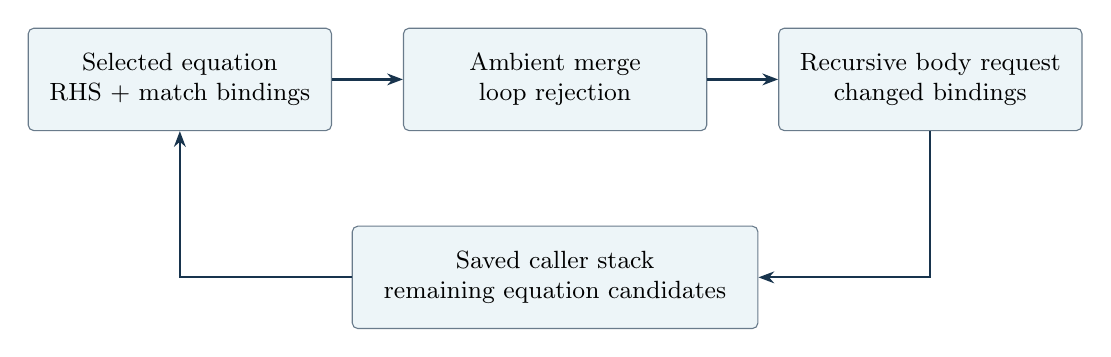
\begin{tikzpicture}
  \node[box] (candidate) {Selected equation\\RHS + match bindings};
  \node[box,right=9mm of candidate] (merge) {Ambient merge\\loop rejection};
  \node[box,right=9mm of merge] (body) {Recursive body request\\changed bindings};
  \node[wide,below=12mm of merge] (stack) {Saved caller stack\\remaining equation candidates};
  \draw[arr] (candidate) -- (merge);
  \draw[arr] (merge) -- (body);
  \draw[arr] (body.south) |- (stack.east);
  \draw[arr] (stack.west) -| (candidate.south);
\end{tikzpicture}
\end{center}
\diagramcaption{Local retained equation execution. The body returns through
the saved continuations; it does not replace its changed bindings by the
pre-call frame. This local realization law is separate from the general
source/contextual correspondence.}

The checked scoped worker now has an earned ordinary-recursion profile in
\name{FirstSuccessScopedRecursiveAdequacy}.  Its three mutually inductive
proof objects cover atom evaluation, left-to-right typed arguments and
ordinary equation rows.  Their interpretation theorem constructs the actual
worker runs; independent structural folds reconstruct
\name{Completed.AtomRel}, \name{ArgumentsRel} and
\name{EquationBodiesRel}, from which the contextual machine runs above any
actual saved continuation.  No constructor accepts either execution as a
premise.  This separation is necessary at recursive returns: one worker
\name{returns} frame represents a boundary batch and the remaining equation
pass that the contextual machine retains as two continuations.  Function
entry is factored through a structural selection agreement, and worker
admissions retain the concrete stacks observed by scoped type freshening.
The top-level theorem drains the
result batch and preserves duplicate answer occurrences and joint
caller/result binding observations.  A two-row control retains both physical
equation occurrences, while a held read under reuse is rejected from this
plain-atom profile.  Ordinary rows include recursively evaluated results,
type-pass leaves, refusal restoration and stopped Empty/Error results.
Complete selected and rejected cast batches share one admission from the
finite worker calculation together with the independent
\name{TypeCastBatchRel} and \name{CastResultRel}, never an assumed transition;
a rejection control retains the whole diagnostic batch.  The nullary
typed-\texttt{f} control in
\name{RecursiveControls} traverses function selection, operator cast, its
physical equation row and publication, then reconstructs the independent
\name{Completed.AtomRel}.  A physical \texttt{g -> f} control exercises the
recursive equation-return constructor with this selected \texttt{f} call
under the unequal continuation representations, reconstructs
\name{Completed.CallRel}, and completes the checked worker in 63 steps.
Function-producing multi-result producers,
branching operator or argument results, and the remaining tuple and minimal
constructors are outside this profile.

Native retained execution supports pause, continuation, inspection and
cancellation. Checked readback components preserve contextual bindings and
distinguish pending computation from written syntax, under explicit
representation assumptions.

The general correspondence still needs arbitrary nesting, scope, quotation,
typed raw arguments, shared choices, branch worlds, demands, ownership,
effects and residuals. Flattened answer equality cannot establish this:
losing a binding world may change a later demand.

\sources{\name{Mettapedia/Languages/MeTTa/HE/RetainedArgumentSpecification.lean},
\name{Mettapedia/Languages/MeTTa/HE/ScopedEquationQuery.lean},
\name{Mettapedia/Languages/MeTTa/HE/FirstSuccessSourceExecution.lean},
\name{Mettapedia/Languages/MeTTa/HE/FirstSuccessScopedRecursiveAdequacy.lean},
\name{Mettapedia/Languages/MeTTa/HE/RecursiveControls.lean},
\name{Mettapedia/Languages/MeTTa/HE/ReflectedStepSharing.lean},
\name{Mettapedia/Machines/BranchLocalNeed/CacheLaws.lean},
\name{Mettapedia/Languages/MeTTa/Bridges/GSLT/CeTTaFrameWriteback.lean}.}
\scope{The model proofs and runtime controls are distinct evidence. They do
not constitute a complete theorem about compiled CeTTa execution, nor freeze
the eventual Prime candidate calculus.}

\subsection*{PeTTa: ordered control through the common interface}

The existing PeTTa evaluator has an explicit configuration: expression or
delivery control, scoped bindings, caller and ordered search frames, the
named-space store, input and output. Its transitions determine which
alternative resumes next and where a selected case commits. The independent
\name{DeclarativeSpec.Runs} judgment records completed answers or a fault
with the reached effect state. No fairness policy is inferred from ordering
the alternatives.

\name{Eval.CommonMachine} packages this actual step function as an
\name{AnswerMachineCore} and uses the existing event-machine adapter.
It lives with the downstream resumption laws; the base source evaluator
does not depend on this adapter.
\name{finished_iff_source} proves both directions between independent source
execution and a common terminal observation; \name{loaded_iff_source} includes
the actual loader. The terminal observation distinguishes a completed
answer list from a source fault. A common \code{finished} outcome here means
that this observation is available, not that the source program succeeded.
\name{final_iff_observed} rules out an unobserved missing-step state.

The adapter publishes logical transition occurrences and retains the complete
configuration at exhaustion. Its \name{resume} law appends only the saved
suffix; controls preserve an effect committed before a pause and keep a
selected empty case body from falling through to another case.
\scope{These laws cover the existing declared closed/saturated source
profile. They do not identify it with PeTTa's eager destination-scoped
\name{EagerDFS} profile, extend it to every open call, or prove a native
SWI-Prolog or C implementation refinement. Those are separate comparison and
coverage obligations.}
The older \name{PrologBridge} dispatches a Pattern evaluator through an oracle;
that interface does not discharge open-query execution or its fresh clause,
DFS and cut obligations. Existing first-order LP substitution and unification
results supply reusable background for that connection.
\sources{\name{Mettapedia/Languages/MeTTa/PeTTa/Eval.lean},
\name{Resumption.lean}, \name{DeclarativeSpec.lean}, \name{EagerDFS.lean};
\name{Mettapedia/Machines/ProductiveCoreAdapters.lean}.}

\subsection*{Complete ordered frontiers for open calls}

The relational source component retains finite-term equations in each branch.
An open call refines these equations jointly with one fresh instance of each
selected clause. Its \name{ClauseChoice.Decision} judgment independently
justifies selection, head mismatch, or absence of a common solution.
\name{Frontier} scans every physical equation position and retains accepted
positions in order. No executable matcher appears in those source judgments.

\name{choices_iff_frontier} proves exact equality of the computed list with a
complete source frontier. Equal equations remain distinct occurrences;
\name{choices_ordered} preserves their source order. Completed empty search
requires a refusal at every position, by \name{choices_empty_iff}.
\name{scope_equation_frontier_iff} joins this source criterion to the retained
scope scheduler in both directions. Clause work precedes the saved alternatives
and preserves their caller constraints, origin paths and reached world.
The law holds for both declared destination policies, so changing their local
evaluation-order choice does not require a new clause-selection proof.

A recursive source equation separates clause coverage from search fairness:
\begin{verbatim}
(= (dfs-loop) (dfs-loop))
!(superpose ((dfs-loop) (quote Later)))
\end{verbatim}
\name{authored_choice_diverges} proves that every finite budget leaves a
saved residual with no published answer. Its proof starts at the source
\code{superpose} entry. The general \name{dfs_loop_every_budget} invariant
retains arbitrary older alternatives, collection scopes and the reached world.
The later value is independently publishable when it is at the head, by
\name{ready_answer_publishes}. Thus a complete list of eligible clauses alone
cannot justify eventual delivery under DFS. The scheduling condition belongs
in the adequacy statement.

Executable controls also cover an aliased open call returning three ordered
occurrences, a pause retaining its two remaining clauses, a completed
incompatible call, and collection retaining duplicate rows while leaving the
caller's variable open. These controls complement the general kernel proofs.

\scope{This is exact open-call entry in the finite relational component.
Whole-program source adequacy, the declared cut boundaries, dynamic syntax and
the complete SWI/native-profile comparison retain their own obligations.}
\sources{\name{Mettapedia/Languages/MeTTa/PeTTa/EagerDFS.lean},
\name{EagerDFSStreaming.lean}.}

\subsection*{Licensed bodies and generative collection}

The existing relational component now has independent local source judgments.
\name{Source.Prepared} specifies body expansion for literals, quotation,
bindings, fixed-head calls and constructors. Its finite demand and scheduling
policies create pending work; they never supply an evaluated child.
\name{prepare_iff_source} proves exact correspondence with the expander,
retaining incoming constraints and the surrounding goal suffix.

\name{Source.Step} independently classifies expansion, accepted and refused
refinement, completed return, inconsistent read states, argument-return
splits, printing and retained operation requests. \name{step_iff_source}
proves both directions at a licensed active goal. This condition is substantive:
\code{collapse}, \code{superpose} and \code{empty} own their scope boundaries.
\name{scoped_form_has_no_local_step} prevents their treatment as ordinary body
work. \name{source_step_scope} and \name{scope_has_local_source} join the local
judgment to the retained dispatcher, with the actual world, context, origins
and older alternatives. Serving a request is a further operational obligation.

Generative operations expose an opaque supply carrier through
\name{FreshOperations}. Their signatures exchange the supply, syntax packets
and protected names. The scoped driver owns caller advancement and world
threading.
\name{CollectionReturn} specifies completion at an empty child frontier,
requiring the independent ordered-copy contract. It resumes the saved caller
with the copied data and its original constraints. The reached world is
preserved. \name{collection_return_iff} proves the maintained finite-supply
operation implements this source boundary in both directions after token
erasure. \name{owned_copies_valid} proves its fresh-copy contract;
\name{shared_residual_copies_refused} rejects reuse of one residual variable
across distinct answer occurrences. Partial child search cannot satisfy the
completion rule.

\scope{The named-parser instance earns its post-reader inventory from the
successful read and owned copy. Source occurrence binding is specified below.
These local source rules compose into the scoped finite execution below;
none verifies the compiled byte reader.}
\sources{\name{Mettapedia/Languages/MeTTa/PeTTa/EagerDFS.lean}.}

\subsection*{Anonymous occurrences bind at the source boundary}

The lexical reader recognizes \code{$_} as an anonymous marker. The scoped
reader first reserves every authored variable name, then expands each marker
to a fresh identity. A named variable retains its identity, including when
it occurs repeatedly. Strings containing the same characters remain data.
\name{Anonymous.Expansion} independently specifies this constructor-preserving
binding traversal. \name{expand_sound} proves the actual traversal satisfies
it, and \name{Expansion.card} counts exactly one new name per anonymous
occurrence. The monotonically extended finite support prevents reuse of an
earlier identity. \name{expand_of_named} proves named-only syntax is unchanged.
The allocator reuses the existing finite-support fresh-string construction.

\name{readExpression_expansion} joins the lexical result to this source
relation and its allocation count. \name{parseAtom_no_marker} proves dynamic
parsing enters the same scoped boundary. The native-shaped Boolean view
commutes with occurrence expansion and preserves the full variable inventory,
so its existing reader-view correspondence remains exact.
\name{loadParsed_named_result} joins that occurrence-bound read to the
existing owned-copy allocator, with no caller-supplied inventory condition.
\name{scope_parse_named_source} recovers the earned source result, token and
exact continuation from the actual retained parse transition under arbitrary
pending alternatives and collection callers. The source operation's
\name{owned_named_parse} law likewise derives this result from its successful
reply; it does not assume a separate raw parse or naming proof.

Controls match \code{(foo $_ $_)} against \code{(foo 1 2)}, while the
repeated named variable rejects that pair. Other controls protect a later
authored \code{$__}, quoted marker text and distinct top-level occurrences.
The retained parsed-pair controls return unequal anonymous variables and
keep a binding to one from constraining the other; the existing repeated-name
controls still share. The machine's continuation grammar and source/execution
correspondence do not change. These are laws of the source reader and its
declared operation models; compiled parser agreement remains separate evidence.

\sources{\name{Mettapedia/Languages/MeTTa/PeTTa/SpaceSemantics.lean},
\name{Mettapedia/Languages/MeTTa/PeTTa/CettaReaderView.lean},
\name{Mettapedia/Languages/MeTTa/PeTTa/StdLib.lean},
\name{Mettapedia/Languages/MeTTa/PeTTa/EagerDFSStreaming.lean}.}

\subsection*{Complete scoped source correspondence}

\name{Source.Invocation} distinguishes local primitive results, parse results,
complete equation frontiers, faults and unserved requests. An equation call
installs its fresh body work before the older alternatives. No constructor
assumes a completed recursive evaluator reply. \name{ActiveStep} combines
these cases with the independent ordinary rules and literal scope entries;
\name{ScopedStep} adds exhausted root search, exhausted child collection and
retained associated-work or allocation requests. Its source configurations
use the existing scope carrier and one shared world.

\name{scoped_step_iff_source} proves exact correspondence with the entire
scope dispatcher for every properly nested configuration. The rule family is
parameterized by local generative operations; the theorem instantiates the
maintained owned supply. Both declared destination policies are covered.

The common productive-block owner supplies \name{Derivation}, a finite
execution judgment over independently supplied local rules. It distinguishes
zero-budget residuals, silent steps, ordered publication, finishing, faults,
requests and explicitly absent transitions. \name{Derivation.sound} composes
local soundness; \name{Machine.derive} composes local reflection and the
continuing-state invariant. \name{Machine.run_iff_derivation} joins them.
\name{Derivation.resume} appends a suffix at the exact saved residual, carrying
earlier publications once and in their original order.

The actual PeTTa instance is \name{Scoped.source_run_iff_derivation}. Every
finite run of the existing scoped streaming adapter corresponds to a source
derivation, in both directions, with identical answer occurrences, reached
bindings, world and retained scopes. \name{completed_iff_source} is its
completed-search specialization. \name{completed_results_unique} compares
completed derivations even at different budgets; their ordered publications
and entire reached configurations agree. The divergent-first-choice control
also has no completed source derivation at any budget. A saved later answer
cannot certify completion of that search.

\subsection*{Commit delimiters and first-success search}

Commitment belongs to the source control state. Each branch records the
boundary of the older alternatives outside its current predicate or
meta-call. This logical delimiter is independent of a native stack address.
Equation selection still earns the complete ordered frontier;
\name{predicateEntry} then installs the callee's delimiter and saves a return
marker restoring the caller's delimiter before its older goals run. The
entry map is injective, so this bookkeeping cannot merge source occurrences.

\code{once} opens a child delimiter, evaluates its child, commits after the
first success, and restores the caller. It does not collect or independently
copy the child's answers. A child failure supplies no caller answer; an
unreachable later success is not promoted past a divergent first branch.
\code{cut} commits at the current predicate delimiter and returns its ordinary
boolean result. These scopes follow PeTTa's translation to Prolog control;
the corresponding host rules are described in the SWI-Prolog manual.\footnote{\url{https://www.swi-prolog.org/pldoc/man?predicate=once/1}
and \url{https://www.swi-prolog.org/pldoc/man?predicate=!/0}.}

For example, the following query retains the outer alternative and produces
the ordered answers \code{A}, \code{Outer}:
\begin{verbatim}
 !(superpose ((once (superpose ((quote A) (quote B))))
              (quote Outer)))
\end{verbatim}
Pruning the whole frontier at \code{once} would lose \code{Outer}.

The independent source commit rule names a split of the pending frontier into
a younger prefix and the retained outer suffix. \name{scope_commit_split}
proves the actual scope step keeps that suffix exactly, together with the
current bindings, source origins, reached world and parent scopes.
\name{scope_commit_invalid} retains a malformed delimiter as a control
request; it cannot become completed failure. The existing local and scoped
correspondences, finite source derivations, completion and resumption laws
extend through the new rules for both destination policies. The recursive
DFS invariant now accounts for the growing saved return-marker stack.

The lifetime adapter uses that actual delimiter step. Let $C(s)$ inventory
the contexts in all retained frontiers and saved collection callers, and let
$P$ be the externally pinned owners. The retired set is
\[
  D=C(s)\setminus(C(s')\cup P).
\]
\name{commit_context_support} proves that $C(s)$ is the union of the
younger-prefix contexts with $C(s')$. A discarded occurrence therefore does
not retire a context still used by another occurrence, a parent or a caller.
\name{commit_lifecycle_square} constructs the independent source cut and
applies the existing \name{OwnedLifecycle.closeScope} to $D$. Every complete
cell reachable through a surviving owner's roots is preserved, including
shared descendants and cycles; the reached semantic world is unchanged.
Checked controls retain duplicate outer occurrences, a collection caller,
an external pin and prior output. Cancelling every context named in the
discarded prefix instead destroys a still-needed shared graph. This local
interface law assumes the supplied ownership roots; it neither discovers all
native strong roots nor authorizes cancellation of an external service.

The general \name{commit\_first\_answer} law starts after the first child
answer reaches its commit boundary. Three logical inspections discard the
named younger prefix, restore the saved delimiter and record that answer,
preserving its bindings, origins, reached world, allocator, outer alternatives
and parent scopes. A root answer is published immediately; a nested collection
retains it internally. No termination or exhaustion premise is imposed on
the discarded siblings. \name{commit\_first\_answer\_source} constructs the
corresponding independent finite source derivation. These laws neither
assert that a first answer exists nor grant permission to cancel an external
service.

The controls cover nested commitment, surviving outer alternatives, later
predicate clauses, failure after cut, quoted cut, collection-local cut,
variable correlation and first success before a divergent later branch.
An actual saved checkpoint already contains its printed effect; its resumed
suffix produces the answer without repeating that effect.
\name{protected_cut_source} and \name{local_cut_source} additionally construct
completed source derivations checked in Lean. Their public observations
differ, proving that the delimiter cannot be erased from the logical state.
Return markers add declared logical transitions; no physical runtime cost
claim follows from those counts.

\scope{These theorems cover the declared finite destination profiles and their
local operation instances, at arbitrary scope nesting. They do not establish
full SWI-PeTTa conformance, the remaining dynamic
or conditional-control admission, global world/freshness and authority invariants, or
native implementation refinement. Unknown operations remain explicit
requests. The native saved-state view carries the logical delimiter; decoding
it from native control remains a realization obligation. Fixed DFS order is
not a fairness or effect-commutation theorem.}
\sources{\name{Mettapedia/GSLT/Distinction/ProductiveBlocks.lean},
\name{Mettapedia/Languages/MeTTa/PeTTa/EagerDFS.lean},
\name{Mettapedia/Languages/MeTTa/PeTTa/EagerDFSStreaming.lean}.}

\subsection*{A shared clause-entry boundary}

Native lowering can reuse a structural matching law without identifying the
whole dialects. \name{ConstructorMatch.petta_match_he_pending} starts with an
actual PeTTa match of a constructor pattern against ground data and constructs
an HE query-matcher occurrence. Its \name{petta_match_he_pending_exact}
strengthening constructs exactly one such occurrence at every larger matching
depth. This is the equality-grounded matcher profile; it does not bound an
extensible custom matcher or combine distinct stored equation copies.
One resulting HE binding record agrees with
every source lookup and materializes the complete pending tuple. The records
may store assignments in different orders. Nonlinear patterns remain admitted;
PeTTa's special \code{cons} list view is excluded at every pattern position.
The converse \name{he_match_petta_pending} reflects an actual HE matcher
occurrence while preserving that same record's whole-tuple readout.
\name{petta_mismatch_iff_he_empty} identifies a PeTTa mismatch with absence of
HE matches at every depth. An empty zero-depth prefix alone supplies no such
evidence. These are clause-entry/readout laws, not recursive program
equivalence or a completed program-search theorem.

The comparison also has an independent equation-model boundary.
\name{petta_match_iff_solution} characterizes constructor-match success by
satisfiability of the pattern equation on ground query data.
\name{query_occurrence_he_pending_exact} obtains that model from an
independent query occurrence's actual result conjunction and constructs the
exact HE matcher frontier together with the PeTTa tuple readout.
\name{no_query_occurrence_of_petta_mismatch} excludes a rejected chosen fresh
instance.

The comparison now also covers complete finite source selection with open
queries and alias-bearing callers. The source-level
\name{petta_accepted_iff_he_candidate} constructs HE matching and logical
conjunction from a PeTTa constraint model, and constructs a PeTTa model in the
reverse direction. \name{he_candidate_petta_solutions} equates their full
solution theories, including every future observation of the caller store.
No variable-representative equality is assumed.

The continuation boundary uses the reached theory rather than restarting
from the caller's initial record. \name{petta_reached_refinement} constructs
the next HE candidate from an actual PeTTa source refinement and preserves
the complete solution relation for the following sibling. Its refusal law
reflects absence of any compatible HE candidate. A control first binds an
open caller variable to \code{A}; the next sibling's alias cannot then match
\code{B}. Reusing the initial caller instead would admit that match.
\name{source_equate_he_pending} connects the law to the actual destination
equation step. A head's certified packet materialization remains valid after
the next refinement, and one environment reads the entire packet of caller
variables, saved values and pending siblings. The result is joint observation
equality, not equality of independent marginal values or residual spellings.

PeTTa's allocator is injective on the finite names used by a clause; HE's
source alpha-variant asks for a globally injective name function. A finite
injective map extends to a permutation without changing the pattern or body.
\name{protected_petta_clause_he_alpha} therefore earns HE's unchanged source
freshness judgment from the actual PeTTa allocator after protecting the
complete finite caller scope. A second constructed permutation relates any
two legal variants while fixing that caller. It proves that refusal at one
variant excludes every other legal spelling.

\name{petta_choices_he_frontier} lifts these row decisions over the actual
complete ordered selector. Its incoming stores are related by their complete
solution theories, allowing different constraint records after an earlier
refinement. \name{reached_head_then_frontier} connects an actual open-alias
source refinement to the following complete query using that earned relation.
Its paired work items retain the same source
positions, fresh bodies, older caller goals, destinations, reserved names and
commit delimiters. \name{petta_choices_he_occurrences} proves that every
completed HE source frontier has the same occurrence bag. In particular,
equal stored equations at distinct positions remain distinct copies.
\name{protected_petta_choices_he_pending} preserves the bag of source
positions paired with these joint packet observations over the actual
complete frontier, protecting the pending packet before freshening.
Its duplicate-clause control retains both occurrences
with a nonempty aliased caller and arbitrary pending operands. This composes
clause selection with local constraint continuation; it does not yet prove
arbitrary open recursive language equivalence.

A PeTTa private result destination need not exist in the HE store.
\name{private_destination_pending_observations} hides a fresh destination
by extending the source model only at that name, while preserving one
joint value/caller packet through the existing valuation-congruence laws.
Its incoming relation already permits private destinations from earlier
returns. \name{petta_joint_refinement} constructs an HE
matching candidate from equality of joint operand/continuation observations;
complete-store agreement and identical operand syntax are unnecessary.
Success and refusal are reflected at this boundary.
\name{source_private_destination_pending} constructs the two actual source
equation steps that introduce a fresh destination and match through it,
while HE matches the value directly. Reusing a public variable as that
destination has a negative observation witness. This is a local source
composition law consumed by the completed recursive source-tree comparison
below.

\name{joint_pending_prepend_fresh} constructs model extensions for fresh
clause syntax on both sides of the scoped relation. Pattern and body share
one interpretation of their variables. The scoped success and refusal laws
then give \name{petta_selected_joint_row}: an actual PeTTa selection
constructs the HE source row at the same stored occurrence, with joint
observations of its reached body and caller.
\name{protected_petta_selected_joint_row} earns the freshness premises from
the existing allocator after protecting both packets and the incoming
binding support. Clause variables are private; matching may still constrain
public caller variables.
\name{protected_petta_joint_choices_he_frontier} folds those proved local
laws over the actual complete PeTTa clause selection and constructs the
complete HE source frontier. Its scoped relation preserves the joint reached
body/caller observations and the multiset of source-position occurrences,
including duplicate clauses. A control combines an open aliased caller,
a past private result destination, duplicate matching clauses and a refused
different head. The two frontier comparisons reuse the same generic fold;
there is no second matching semantics. These local laws feed the recursive
source-tree comparison below.

The existing scoped PeTTa machine also has a source-level continuation
attachment law. A saved goal suffix is protected before fresh allocation;
attaching it shifts each saved argument-return depth by its length.
\name{ProtectedContinuation.preReturn_derivation_attach} transports an
arbitrary finite ordinary recursive prefix through this attachment. Complete
equation frontiers, including rejected alternatives and duplicate source
paths, retain their reached constraints. Only the current child's work gains
the suffix; parent scopes and collected answers remain unchanged.
\name{preReturn_return_continuation_iff} joins this prefix to an actual returned
head and an independent suffix derivation. The reached binding equations,
world, context, origins and pending frontier initialize that suffix.
\name{preReturn_continuation_run} executes the actual machine from the
reached cut, preserving the reached world instead of repeating the prefix.
This source profile admits local silent steps, refusals and complete ordinary
equation invocations. Local printed output is retained; external primitive
replies, child collections, cuts and terminal answer publication are outside
the prefix transport. Its terminal inversion is the independent source law
\name{Source.Step.returned_iff}; no continuation adapter supplies a second
definition of source return.

Open child values must be observed together with their unevaluated siblings
and caller packet. \name{Destination.solutionTuples} is the canonical
all-model source observer. \name{resolve_read_preserved_by_extension} proves
that a materialized open value retains its meaning in any later model
extending the reached equations. The head is not frozen to a separately
chosen value before the remaining siblings run.

\name{OpenContinuation.OpenSpine.transport} uses this boundary for a common
tuple/typed-argument spine induction. Each head has an independent HE child
derivation and an actual retained scoped PeTTa path. The proof reconstructs
the existing HE \name{TupleRel} or \name{ArgumentsRel}; it reads the whole
evaluated prefix in each final tail frame. Thus later siblings can refine an
earlier open variable while its correlation with the caller remains intact.
The saved continuation contains the final equation or invocation goal:
\name{assembled_equate} consumes its reached equation cut, and
\name{call_frontier} constructs the complete protected clause frontier with
physical positions and duplicate occurrences.

The earned recursive closure is
\name{OpenRecursive.Evaluation.transport}. Five mutually inductive source
judgments describe evaluation, arguments, argument alternatives, invocation
and clause bodies. Every defined call carries a complete
\name{ClauseChoice.Frontier}; no child-completion callback occurs in the
induction. Their forward theorems construct the existing HE
\name{AtomRel}, \name{TupleRel}, \name{CallsRel} and
\name{EquationBodiesRel} derivations. \name{Evaluation.paths} reconstructs a
source branch path to every outcome. A \name{List.Forall2} outcome relation
gives exact ordered equality of the joint observation packets, hence also a
multiset equality which preserves duplicate occurrences.

Fresh allocation is split at its actual boundary. A
\name{PrivateDestination} is fresh for the reached equation store and its
input syntax. Its saved continuation intentionally mentions the destination,
because that is the child's return channel. \name{Evaluation.Allocated}
separately protects the evaluated prefix and pending caller packet at every
recursive cut. This split is required for nonempty argument lists and is
exercised by the positive recursive control.

There is also a genuine source-policy boundary at an open variable entry.
\name{active_binding_separates_dispatch} uses the pure rule
\code{(= (f) A)} and a certified active binding \code{x = (f)}. Both source
stores agree on every joint observation packet, but HE reads then evaluates
\code{$x} to \code{A}, whereas PeTTa's variable rule returns \code{(f)} as
data. The program satisfies the existing scoped code admission. Consequently,
model agreement cannot supply arbitrary open-child evaluation correspondence.
\name{AtomRel.input_read_eq} gives the valid HE transport law: the complete
reached read, including readiness, must agree. A larger shared open fragment
therefore needs an explicit compatible evaluation profile as well as earned
recursive occurrence coverage; changing binding representatives alone does
not resolve this separator.

Passive captures supply the structural variable-entry profile.
\name{PureConstructor.Value} admits constructor data with an explicit scope
of free names; its empty-scope instance is the existing closed-value profile.
One completion induction, \name{Value.he_completes_unassigned}, serves both.
\name{PassiveEnvironment} requires passive, error-marker-free stored values.
Its substitution, binding and unifier preservation laws follow actual
materialization and both binding orientations. Call-expression matching
requires passive child symbols and arguments, so a defining outer head need
not itself be a passive application. Certified normal readout then earns
bound-variable evaluation. \name{OpenContinuation.passive_variable_child}
constructs the actual two scoped source steps after any evaluated prefix,
preserving the joint packet and every retained caller component. A positive
control stores an open held constructor; the active-call separator is excluded
for every name scope. The existing \name{CodeRel} admits scoped passive
captures and restricts substitution to such captures; its read and scope
extension laws preserve admission across materialized siblings. Active
applications retain a literal ordinary head. A computed variable head can
become a defining call under HE's initial read while PeTTa retains its raw
non-symbol-head data dispatch. The comparison excludes that syntax through
\name{CodeRel.no_variable_head}, without changing either source semantics.
Open clause entry also needs passive patterns: unification may bind a caller
variable to a pattern subterm. \name{ConstructorPatterns} requires ordinary
heads and passive, error-free argument patterns. Its frontier law inherits
the actual source row and transports that admission along its alpha-variant.
\name{ConstructorPatterns.clause_entry} then earns both a passive reached
environment and admitted materialized body, in the caller scope extended by
the fresh pattern names. It uses actual unification and no child-completion
premise. The existing closed body-admission proof factors through the common
\name{CodeProgram.work_body_code} law. The recursive duplicate-clause control
satisfies the admission; a pattern containing an applied defining head is
rejected. The recursive source-tree induction consumes these closure laws at
every selected clause.
\[
\begin{array}{ccc}
 \text{PeTTa ordered clause work}&\longrightarrow&\text{HE source frontier}\\
 \downarrow\scriptstyle\text{source positions}&&
 \downarrow\scriptstyle\text{source positions}\\
 \text{occurrence bag}&=&\text{occurrence bag}.
\end{array}
\]
The principal positive control evaluates open \code{(fork \$x)} under
\code{x = Z}. It enters both identical physical clauses, recursively evaluates
\code{strip}, and assembles \code{Box Z}. The theorem constructs two result
occurrences and their branch paths, proves exact ordered packet equality,
admits the joint observation \code{[Box Z,Z]}, and rejects
\code{[Box Z,S Z]}. Thus duplicate multiplicity and caller correlation are
both non-vacuous. The active-bound-call and active-pattern examples remain
the negative admission boundaries.

Deterministic \name{CollectionScope} DFS linearization is factored from that
branch-tree induction. \name{BranchTrace} records the physical source-position
path of every outcome. \name{DelimitedControl} relates a raw source control to
the actual scoped control whose active prefix is followed by a finite stack of
\name{restoreCommit} delimiters and then its concrete outer continuation. It
uses separate source and concrete continuations, so an argument's unevaluated
siblings remain before an enclosing delimiter stack. Delimiter goals contain
no atoms; the relation therefore preserves control support, fresh-name choice
and fresh-slot allocation exactly.

The live freshness set is derived rather than guessed.
\name{pendingSupport} and \name{collectedSupport} factor the concrete
\name{collectionSupport} into the active control, queued suffix and retained
answers. The five mutually recursive \name{ExtraSynchronized} predicates
verify that every equation node uses this exact set. Their corresponding
\name{drain} theorems construct the retained scoped path for evaluation,
arguments, argument alternatives, invocation and clause bodies.
\name{RootContinuationContract} preserves the allocator, world, parent scopes,
outer pending work and occurrence origins while appending answers in source
order. Its continuation algebra is the existing
\name{OrderedStateFlatMapRel}; no second scheduler or supplied machine run is
introduced.

The principal composition theorem \name{Evaluation.realize_root} applies the
HE transport and the PeTTa queue drain to the same admitted recursive source
tree. It earns the HE \name{AtomRel}, ordered joint-packet correspondence,
every branch path and the executable retained DFS contract. The recursive
fork/strip control computes its freshening profile in queue order: its first
recursive call protects the second selected clause, while its second protects
the first collected answer. \name{open_recursive_duplicate_realization}
constructs both realizations, retains the two physical origins, admits
\code{[Box Z,Z]} and rejects \code{[Box Z,S Z]}.

Exhausted calls give a small separation witness. With the sole equation
\code{(= (f A) OK)}, both implementations return \code{OK} for \code{(f A)}.
HE retains \code{(f B)} when no clause matches the defined head; PeTTa returns
no answer. Both retain \code{(unregistered B)} when its head is entirely
undefined. Thus a common eager fragment must justify the coverage of each
reached defined call, or explicitly translate this difference. An answer-bag
quotient cannot erase a residual value versus no value.
\sources{\name{Mettapedia/Languages/MeTTa/Translation/HEPeTTaNativeLoweringContracts.lean};
\name{Mettapedia/Languages/MeTTa/Translation/HEPeTTaOpenRecursive.lean};
\name{Translation/he_petta_defined_miss.metta}.}

\subsection*{Recursive source completion and tuple-protocol separation}

\name{PureConstructor.Evaluation} is a finite, proof-relevant source tree
for ordinary eager constructor programs. Its mutually defined argument,
invocation and body families account for complete structural clause scans,
physical row positions and recursive child completions. Every argument answer
finishes its continuation before the next answer is explored. The tree is
independent of machine transitions, runner fuel and evaluator callbacks.
Typed demand, primitive/control heads, the special \code{cons} list view and
exhausted calls to a defined head are outside this candidate shared fragment.

The checked \name{Evaluation.petta_path} constructs an actual path of the
maintained PeTTa machine for every such tree in an annotation-free program.
\name{Evaluation.petta_source} connects that path to the independent completed
\name{PeTTa.DeclarativeSpec.Runs} judgment, preserving the entire ordered
answer list and the initial pure world. All five mutual families have path
theorems; the recursive bodies are not left as assumed evaluator replies.
\name{Evaluation.petta_completed_iff} characterizes every completed machine
observation from a load with such a source tree, including its whole store
and I/O. It does not claim source-tree admission for excluded programs.
The control \name{duplicate_recursive_petta} proves the exact two-answer list
for two identical stored \code{fork} clauses, each invoking a recursive
\code{strip} on a constructor natural, at every natural-number input depth.

\name{Evaluation.values} derives the passive return contract from the whole
source tree. \name{Evaluation.answer_read_exact} then preserves any annotated
representation of an answer through every certified HE frame and every
declared rebuilding policy. The generic source law
\name{Frame.read_variable_free} proves that result without examining binding
storage. \name{ConstructorHead.he_frontier_empty} also constructs complete
HE absence evidence against the actual equation table for an undefined
constructor head, with arbitrary retained caller constraints.

These connections do not establish unrestricted recursive HE equivalence.
Two source controls locate a precise obstruction. Active \code{(Empty A)}
reaches HE's empty marker, whereas explicitly held syntax is reused under the
ready policy. \name{no_atom_only_ready_evaluator} proves that erasing readiness
cannot define a complete evaluation state for that policy.

The return base case now has a constructed HE connection.
\name{Value.he\_completes} evaluates arbitrarily nested passive data with
unchanged syntax and the same certified frame, allowing every nested
occurrence status and every declared local policy. Its output annotations
come from HE's actual publication constructors. The explicit
\name{NoErrorSymbol} admission excludes the scalar-tag collision described
below; it is checked on the materialized value, not merely its raw template.
\name{Value.he\_return} joins that phase to the full return boundary.

\name{passive\_equation\_call} then constructs a complete HE call from its
physical frontier when the binding constraints determine passive body
instances. Contextual unifiers and certified frames are constructed from the
source candidates. Each stored work occurrence produces one result, retaining
its reached binding record; no complete evaluator reply is an assumption.
The duplicate-call control proves this for every certified caller, including
nonempty alias-bearing callers. It does not assert that arbitrary recursive
equation bodies are passive.

Fresh-body materialization is also representation-independent.
\name{ReadoutCertificate.forced\_read} proves that a value forced by all models
of a constraint record is the literal read of its retained certified table.
\name{query\_occurrence\_template\_readout} derives the read for an actual
selected source occurrence from a closed query, one source pattern instance
and coverage of body variables by the pattern:
\[
\begin{array}{ccc}
 \text{raw body}&\xrightarrow{\ \text{source substitution}\ }&\text{materialized code}\\
 \downarrow\scriptstyle\alpha&&\Vert\\
 \text{fresh body}&\xrightarrow{\ \text{certified frame read}\ }&\text{materialized code}.
\end{array}
\]
\name{frontier\_body\_read} applies that square to the actual work occurrence
and reached contextual frame. The materialized code may itself contain further
calls. \name{Evaluation.substituted} constructs the corresponding finite
source tree with its input substitution moved into syntax, preserving its
complete answers. A positive control keeps two uses of one fresh variable
correlated through any qualifying table; a negative control shows why an
escaping body variable is not determined by its pattern.

Complete structural clause scans now construct that HE frontier directly.
\name{fresh\_pattern\_model} combines any satisfiable caller model with a
fresh rule model, preserving the caller on its entire constraint support.
On closed ground query data,
\name{fresh\_candidate\_iff\_source\_match} equates viable HE candidates
with the independent structural source match. The shared match specification
owns the substitution-stability and ground-roundtrip laws used here; the
inversion development imports them rather than duplicating them.
\name{ClauseScan.he\_frontier} then constructs every selected physical
work item and excludes every omitted row under all legal fresh spellings.
Its pairing retains the original clause position, raw body and actual source
substitution image. No evaluator answer or implementation record is supplied
to this construction.

The explicit \name{RangeRestricted} admission covers body variables by their
own raw pattern. \name{ClauseInstance.body\_model} proves that every model of
the reached work item reads its fresh body as that source substitution does.
The code so obtained may contain further calls. The control
\name{duplicate\_recursive\_frontier} retains positions two and three and
the exact two recursive tail calls at every constructor-natural input depth,
with arbitrary certified caller constraints.

\name{fresh\_candidate\_caller\_theory} and
\name{ClauseInstance.caller\_observations} also preserve the existing
\name{BindingTheoryEquivAt} observer on the full visible query, live
continuation and incoming constraint scope. Every caller model extends to a
model of the selected private constraints with the same protected values;
every reached model restricts to a caller model. Equality of binding records
or representative names is unnecessary. An open-assignment counterexample
shows why this unchanged-caller law requires a closed query: a public query
variable may legitimately acquire a new binding.

For passive instantiated bodies and passive argument syntax, the composition
reaches the full evaluation boundary.
\name{values\_he\_tuple} reuses the nested data proof as a complete annotated
tuple packet. \name{ClauseScan.he\_passive\_evaluation} joins that traversal
to clause selection, return, reached-frame readout, success priority and
publication, under every declared local policy.
\name{ClauseScan.passive\_completed\_pair} constructs completed HE and PeTTa
source evaluations with the same entire answer list from the same admitted
source work. The operational bridge's \name{ClauseScan.passive\_machine\_pair}
composes these derivations with the existing correspondence laws, constructing
a path of the retained HE machine and a sufficient-fuel PeTTa run with those
same answer occurrences. Every published result additionally preserves the
protected caller-binding observer. It introduces no additional machine or evaluator.
The captured-variable control uses its argument twice in each
of two equal stored clauses, obtaining two equal data results for every
certified HE caller. The raw-variable counterexample shows that omitting
fresh instantiation can instead conflict with a satisfiable caller.
The recursive construction now extends beyond that passive-body result.
\name{CodeRel} distinguishes active source syntax from passive annotated
data and records the scope of variable leaves. Its renaming and substitution
laws retain every nested readiness mark under either rebuilding policy.
\name{CodeProgram} admits each raw rule body in its pattern-variable scope;
it is a syntactic condition, not an evaluator postcondition or a termination
assumption. Actual structural matches earn their safe captures and variable
coverage. \name{ClauseInstance.body\_code} then derives closed executable
code for the fresh body in the reached certified frame, with the same
materialized syntax as the source substitution. No recursive result is a
premise of this transport.

\name{RecursiveTransport.he\_evaluation} constructs a complete HE batch
from every admitted finite source tree. Its five-way induction composes
expressions, arguments, argument alternatives, invocations and recursive
bodies. It retains the entire ordered answer occurrence list and each actual
result frame under every declared local policy. Tuple assembly reuses HE's
existing tuple and call judgments; it does not introduce another evaluator.
\name{Evaluation.recursive\_machine\_pair} joins this construction to the
maintained HE and PeTTa machines, preserving the pure world and complete
answer list. The \name{nested\_recursive\_completed\_pair} control proves
four equal answers when two separate argument positions each run a recursive
binary choice, at every constructor-natural input depth and for arbitrary
certified HE callers. \name{held\_recursive\_call\_not\_admitted} supplies
the opposite readiness control.

The reverse direction now has two general base laws. The independent
\name{EquationFrontierRel.source\_related} pairs every two complete scans
of the same stored presentation by physical position, raw pattern and raw
body. \name{ClauseScan.he\_frontier\_all} transports the structural source
scan to every such HE frontier, without requiring equal private names or
constraint records. \name{RecursiveTransport.passive\_atom\_exact} and
\name{passive\_tuple\_exact} characterize every completed phase on admitted
passive data: there is one value with the same erased syntax and the same
caller constraint record. They retain the actual reached annotated value
and certified frame; they do not identify alternate environment layouts.
The source type owner supplies complete-query uniqueness and the exact
undefined-demand cast law. \name{AtomRel.undefined\_operator\_phases}
exposes tuple/call/publication children for either presentation of undefined
operator selection, under every declared local policy.

\name{RecursiveTransport.he\_evaluation\_exact} proves the universal reverse
answer law. For any admitted finite source tree and closed annotated input,
every completed HE phase has that source tree's entire ordered answer list.
The five mutual proofs invert the actual tuple, alternative, invocation and
body phases, pairing every complete physical frontier with the independent
source scan. They retain arbitrary certified callers and all declared local
policies; a recursive evaluator's desired answer is never a premise.
\name{Evaluation.recursive\_machine\_observation\_iff} composes this result
with the maintained HE machine's completed-path correspondence and PeTTa's
independent completed-observation theorem. A complete HE answer observation
exists exactly when the PeTTa machine completes with that same ordered list
and unchanged pure world. \name{nested\_recursive\_completion\_exact}
characterizes every completion of the four-answer control at every input
depth, and \name{nested\_recursive\_cannot\_drop\_choice} excludes a
two-answer completion.

The ordered equality above is a presentation law for one fixed equation
traversal. The public completed HE observation is its multiset quotient,
retaining duplicate occurrences. \name{recursive\_machine\_bag\_iff}
compares that bag with the bag view of PeTTa's completed ordered execution;
it does not erase PeTTa's operational prefixes. The stronger storage law is
separate. \name{Evaluation.perm\_program} transports an independent finite
source tree across any permutation of the stored equation copies, including
nested alternatives and recursive bodies. Clause positions are recomputed,
while each selected substitution/body pair is retained with its multiplicity.
\name{recursive\_machine\_storage\_permutation} composes this construction
with both directions of machine adequacy. It thus preserves completed HE
bags without assuming termination of the reordered computation. The control
\code{[A,B,A]} versus \code{[B,A,A]} distinguishes list order from bag equality
and rejects dropping the duplicate. These laws apply to the declared pure,
annotation-free fragment. First-applicable type selection and effects retain
their declared enumeration and causal order; a bag observer alone cannot
justify reordering them.

The recursive proofs also compose the caller-binding observer.
\name{ConservativeExtension}, in the existing binding-observation owner,
retains all incoming constraint support and compares models on that support
together with the protected continuation names. Its transitivity law keeps
earlier support visible to later fresh instances, including tautological
constraints. \name{ClauseInstance.caller\_extension} earns the invariant
from actual selected source work. The five inverse laws carry it through
argument alternatives, recursive bodies, return and publication, without
requiring equal environment layouts or private representatives.
\name{he\_evaluation\_caller\_observations} projects the complete
\name{BindingTheoryEquivAt} observer on the visible query, live continuation
and incoming constraint scope. Every completed machine path satisfies the
same law through \name{Evaluation.recursive\_machine\_caller\_observations};
\name{recursive\_machine\_pair} constructs both runs with that observer.
The all-depth \name{nested\_recursive\_caller\_observations} control includes
arbitrary certified callers. \name{visible\_assignment\_refused} proves that
assigning a previously unconstrained protected name fails this invariant.
These answer and binding-observation laws establish the declared recursive
comparison fragment; they do not extend its admission to either full dialect.

The second obstruction remains even with no equations, bindings or effects:
\[
 \code{(Box Error A)}
 \quad\begin{cases}
  \longmapsto \code{(Error A)} & \text{HE completed tuple rules},\\
  \longmapsto \code{(Box Error A)} & \text{PeTTa completed source}.
 \end{cases}
\]
HE's published \code{interpret\_tuple} rule tests the recursively assembled
tail for the \code{Error} shape before prepending its head. It consequently
propagates the successful tail \code{(Error A)} as a failure and discards
\code{Box}. \name{he_propagates_assembled_error_tail} proves this derivation
for every declared marking policy; \name{petta_retains_error_tail} proves the
other observation independently. Installed Rust HE 0.2.10 and SWI-PeTTa
reproduce the respective observations on the tiny discriminator. This is a
source-protocol separation, not a claim about a backend storage defect.

A stronger shared fragment must therefore constrain such control-shaped
data or translate the protocol. A distinct internal success packet carrying
tuple elements would remove this collision; propagating only tagged failures
would deliberately change the displayed HE observation. That is a local
semantic proposal, not an established compatibility result or a change to
the faithful source rules. The constructed recursive join uses this explicit
admission; it does not establish equivalence for the separating program or
for either unrestricted dialect.
\sources{\name{Mettapedia/Languages/MeTTa/Translation/HEPeTTaSound.lean},
\name{Mettapedia/Languages/MeTTa/HE/Spec/Eval.lean},
\name{Mettapedia/Languages/MeTTa/PeTTa/Eval.lean};
\name{Translation/he_petta_marker_head.metta},
\name{Translation/he_petta_recursive_duplicates.metta}.}

\newpage
\section{GSLT and rho: retain searches, publish occurrences}

An authored language also reaches the common execution interface through
the existing GSLT-to-MeTTa bridge. Under its explicit first-order, provider
and premise admission conditions,
\name{observes_contextual_iff_gslt_step} relates the actual PeTTa source
judgment to the independent GSLT step. The corollary
\name{common_machine_observes_contextual_iff_gslt_step} composes that result
with PeTTa's common-machine adequacy: a completed run returns the encoded
reduct frontier, and membership in that frontier is equivalent to a licensed
source step. The evaluator budget and the recursive-premise depth remain
separate parameters. The ordered frontier retains repeated witnesses;
the source step's membership observation alone does not count them.

This connection does not identify every syntactic context with an evaluation
context. Authored operational premises license reduction; equations use
their independently admitted congruence contexts. The emitted runner and
graph entrypoints additionally have exact PeTTa return theorems. Their
current reachability-completeness clauses require no declared collection or
scope-extrusion laws. The presented-semantics development supplies forward
soundness with those laws, under \name{ExtrusionsFlatten}; the broader
operational coherence and completeness result is separate. Visited-state
deduplication in that explorer preserves reachability, not the number of
derivation paths or answer occurrences.

\sources{\name{Mettapedia/Languages/MeTTa/PeTTa/Bridges/MeTTaIL/ContextualRuleExecution.lean},
\name{Mettapedia/Languages/MeTTa/PeTTa/Bridges/MeTTaIL/CompleteEmissionExecution.lean},
\name{Mettapedia/OSLF/MeTTaIL/Complete/Presented.lean}.}

The scoped GSLT scheduler advances actual premise, matcher and query frames.
It retains pending tasks, proved results and unresolved obligations.
PeTTa's authored program driver packages these searches into resumable jobs.
Its aggregate and publication are deliberately distinct: a later job may
already have results while an earlier incomplete job still controls their
public order.

\begin{center}
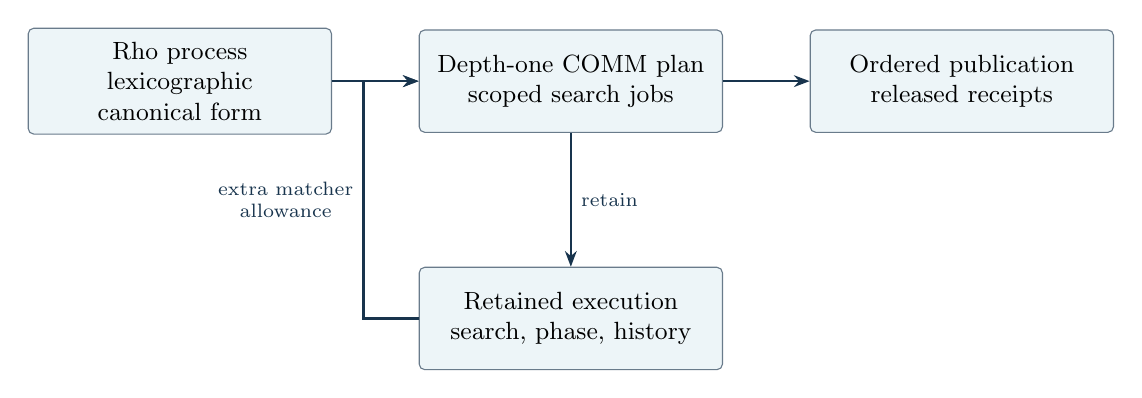
\begin{tikzpicture}
  \node[box] (proc) {Rho process\\lexicographic canonical form};
  \node[box,right=11mm of proc] (jobs) {Depth-one COMM plan\\scoped search jobs};
  \node[box,right=11mm of jobs] (pub) {Ordered publication\\released receipts};
  \node[box,below=17mm of jobs] (search) {Retained execution\\search, phase, history};
  \draw[arr] (proc) -- (jobs); \draw[arr] (jobs) -- (pub);
  \draw[arr] (jobs) -- node[hint,right]{retain} (search);
  \draw[arr] (search.west) -- ++(-7mm,0) coordinate (retry)
    -- node[hint,left]{extra matcher\\allowance} (retry |- jobs.west) -- (jobs.west);
\end{tikzpicture}
\end{center}

The actual \name{rho:run:resume-search} equation advances the pending
\name{ProgramObservation} and returns the full updated \name{RhoSearch}.
The evaluator-return and completion theorems cover that quoted equation,
including unchanged ambient state and empty effect queues.
\name{Search.resume_valid} retains earned validity, and publication grows
by prefix.

A released receipt supplies a source-valid rho step modulo structural
congruence. The existing \name{step_sound}, \name{step_quiescent} and saturation
results distinguish a step, quiescence and insufficient search allowance.
Empty publication establishes quiescence only when the search is complete.
Stopping with no answer so far is not evidence that there is no answer.

The shared trajectory law is instantiated by scheduled states and actual
PeTTa jobs/programs:
\[
 \resume(s,m+n)=\resume(\resume(s,m),n).
\]
The units differ: scheduled fuel counts ticks; PeTTa adds allowance per job.
Publication cursors emit only a newly released suffix and keep absolute
occurrence ordinals, including equal-valued duplicate answers.

\sources{\name{Mettapedia/OSLF/MeTTaIL/StructuralDescentScheduledExecution.lean},
\name{Mettapedia/Languages/MeTTa/PeTTa/Bridges/MeTTaIL/GeneralProgramResumptionExecution.lean},
\name{Mettapedia/Languages/MeTTa/PeTTa/Bridges/MeTTaIL/RhoRunnerExecution.lean}.}
Retained \name{Execution} adds successive completed COMM commitment and
cancellation to the search state. A commit selects one completed publication,
records its before/receipt/after triple, and begins a new search for the
successor process. Its quoted \name{rho:run:commit-candidate} equation checks the
entire supplied receipt wire against that local selection. A foreign candidate
or an immediate stale candidate does not extend the history. Resume preserves
the committed prefix; cancellation preserves history and drops live work.
\name{Execution.advance_add} instantiates the shared resumable trajectory.
Its fuel counts commit attempts, including no-ops; matcher allowance is resumed
separately. A two-communication control keeps both commits in chronology.

Every execution reached by any sequence of retained operations is sound
(\name{Retained.Reached.sound}): its history is a chronological sequence of
committed depth-one COMMs from the canonical start (\name{Retained.Reached.chain}),
its live search runs at that history's endpoint, and a done phase there is exact
quiescence. A commit placed at the wrong state, or with a result that is not the
receipt's, is not a chronicle. Under the common owned host
(\name{Retained.owned_publication}) committed COMMs reach the world exactly once,
copies of used tickets are refused, and the delivered history is that chronological
COMM sequence.

Selection need not always use the first published receipt.
\name{commitPublished} validates membership of the complete supplied receipt,
including its matcher, source job, bindings and premise history. Two ground
communications in disjoint multiset components construct a retained diamond
(\name{disjoint_retained_diamond}): each edge is an actual completed search
and licensed commit. Both schedules reach the same process; their chronological
histories remain distinct, with equality only under the declared causal observer.

The local dependency interface names input, output and fresh allocation
occurrences. Distinct keys retain distinct resources even when their process
values coincide. Fresh, live and spent states prevent reusing a consumed key.
The actual read program produces the candidate's dependencies; disjoint
read/write footprints prove that an unrelated commit preserves its validation.
\name{replay_after_history_refused} excludes reusing a consumed occurrence
through any later accepted history. Cancellation closes the owned publication
channel, and stale reads publish no world change even with a current ticket.
The quoted \name{rho:run:commit-published} and cell-store commands have source
execution and store-refinement proofs, as well as matching native controls.
An old whole-process search receipt is never relabelled for the successor:
its search is rebuilt there, while the local dependency certificate can survive
independent updates.

\scope{A commit's independent rho-step licence requires valid search and a
well-typed process. The quoted bridge uses the pinned depth-one COMM plan and
prepared encoded values. The owned host is a sequential model of authority;
durable or distributed exclusive delivery is a host obligation, and fairness over
all alternatives is not proved here.}

\newpage
\section{World queries: what can safely survive a change?}

A pure adaptive query can choose its next read from a previous result.
Its observation therefore contains both its answer and the ordered reads it
actually performed. A read certificate records complete values, including
absence and complete ordered match lists.

\begin{center}
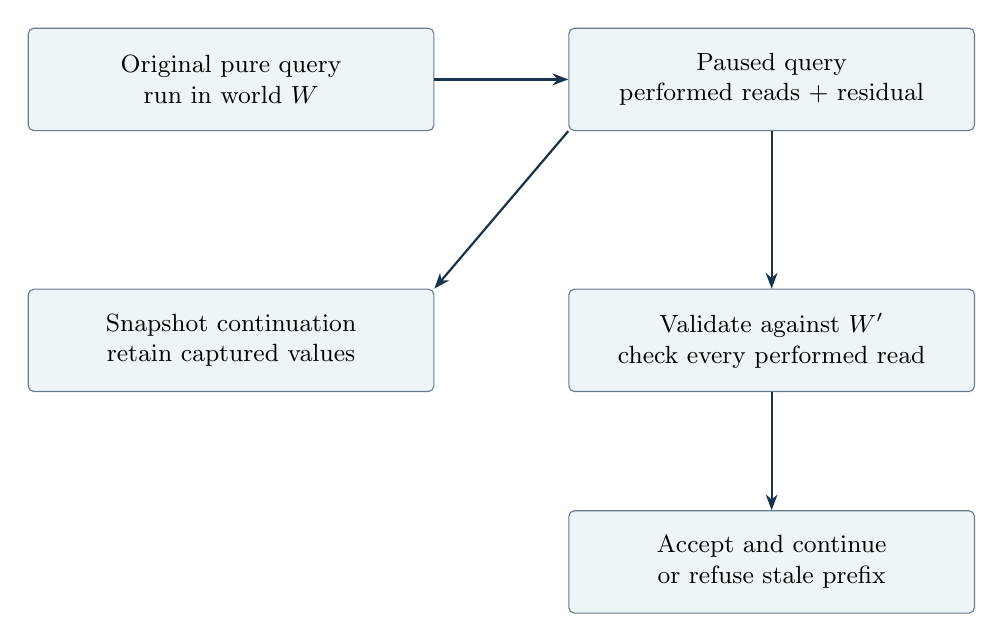
\begin{tikzpicture}
  \node[wide] (query) {Original pure query\\run in world $W$};
  \node[wide,right=17mm of query] (pause) {Paused query\\performed reads + residual};
  \node[wide,below=20mm of query] (snapshot) {Snapshot continuation\\retain captured values};
  \node[wide,below=20mm of pause] (validate) {Validate against $W'$\\check every performed read};
  \node[wide,below=15mm of validate] (continue) {Accept and continue\\or refuse stale prefix};
  \draw[arr] (query) -- (pause);
  \draw[arr] (pause.south west) -- (snapshot.north east);
  \draw[arr] (pause) -- (validate);
  \draw[arr] (validate) -- (continue);
\end{tikzpicture}
\end{center}

Suppose the query reads all matches at a key and gets $[a,a]$. Replacing that
list by $[a,a,b]$ changes the read even though both results are nonempty.
Replacing it by $[a]$ loses an occurrence. Reordering it can change a first
answer. An empty result must also be recorded: a later insertion invalidates
the earlier absence. An update to an unread key can remain compatible.

\name{run_eq_of_agrees} proves that agreement on the complete performed
certificate preserves the query's answer and read path.
\name{Retained.resumeValidated} checks the performed prefix before executing
any pending read. \name{Retained.validated_fresh} connects an accepted earned
prefix to fresh execution of the original query in the new world.

Snapshot continuation is a different policy. A residual may already have
closed over a captured answer, and retains it even when the current store
changes. Failed validation does not retroactively turn that old residual into
a fresh query. Starting the original pure query again is possible; replaying
committed effects to refresh knowledge needs a separate effect contract.

Writes computed from reads follow the same rule. An owner runs a transaction,
a pure query whose answer is a list of writes, on the snapshot it saw and proposes
the writes with the complete read certificate. The ledger commits the proposal
only when every recorded read agrees with the current store. An accepted proposal
writes what its transaction would write now (\name{commit_fresh}), so accepted
commitments are serializable (\name{commitAll_serial}); a proposal is refused
exactly when one of its reads changed (\name{commit_refused_iff}). Two increments
of one counter from the same snapshot commit once; rerunning the refused one on a
fresh snapshot commits it; writing both blindly loses an update. The ledger is a
retained state for the owned host, which publishes each accepted write list once
(\name{ledger_published_once}).

\sources{\name{Mettapedia/Machines/ReadOnlyQuery.lean},
\name{Mettapedia/Machines/ReadCertifiedQueryReuse.lean},
\name{Mettapedia/Machines/ValidatedCommit.lean},
\name{Mettapedia/Coalgebra/CoherentPrefixTower.lean}.}
\scope{This is a pure read interface. Query identity, program revisions,
ownership and service authority are additional dependencies; an unchanged
read list alone does not validate a changed program or authorize consumption.}

\subsection*{Context identity is not a space snapshot}

Two fresh mutable spaces can have equal current contents and still denote
different places to write. \name{ModuleStore.equal_contents_forbid_content_codec}
proves that no payload computed only from those equal contents can recover
both identities. \name{annotation_write_lookup} and
\name{annotation_write_other} give the positive distinction: a write changes
the selected context's lookup and preserves another context's lookup.
The maintained \code{he_context_identity_discriminator.metta} allocates two
empty spaces, writes to one, and asserts that the other remains empty. Rust
HE passes this control; it is an abstraction discriminator, not evidence of
an engine defect.

The existing \name{Contextual.Control} is parameterized by its context-label
carrier. Its work, results and continuation grammar are unchanged.
\name{WorldConfiguration} carries one shared world, the root context identity,
that control, the caller stack and prior publications. \name{snapshot} reads
all currently retained operational context views from the reached world.
It is a phase projection, not an encoding of mutable identity. Its footprint
congruence law and \name{disjoint_context_write_snapshot} preserve a current
read-only phase under writes outside the declared direct-key footprint;
module dependency views need their own complete footprint.

\name{WorldLocalStep} reuses the old ordinary primitive transitions at the
current context's view through \name{UnscopedControl}. Context entry stores
labels, and its nested rule propagates the child's reached world back to
the caller. The three context instructions use the context-label payload.
\name{managedContextControl} prevents the old contents-valued
\code{context-space} path from bypassing that boundary. A \code{call-native}
rule installs a completed local host result and its reached world. Its
contract takes one invocation and a logical activation, without the caller
control or a recursive evaluator. It specifies reply installation; service
execution, reentrancy and cost require their separate refinement laws.
\name{WorldStep} adds the existing ordered root-publication discipline, and
\name{worldSpan} instantiates the same relation-level machine interface.

The read-only instance uses the supplied snapshot service and disables native
completion, as the old completed core does. Local transitions and whole paths
lift and project in both directions. \name{world_readOnly_source_iff_observed}
then preserves the entire existing independent completed source profile,
including nested contexts, bindings and retained continuations. A nontrivial
model native-write instance separately changes an actual context store under
a saved child. \name{nested_native_write_reaches_caller} and
\name{native_return_keeps_reached_world} keep its reached store, activation,
inner and outer continuations and prior publications. No native plugin
implementation is inferred from that model instance.

The independent \name{Completed.Stateful} judgments now thread the reached
world through each completed source phase, including all recursive children,
captured equation alternatives, function returns and context changes.
\name{WorldEnvironment} supplies current context views, casting and local
host contracts; it contains no evaluator. The existing entry, type selection,
logical unification, annotated readout, marking and success-priority judgments
are reused. Remaining alternatives are the frontier captured before their
children execute; later queries use their actual reached world.

In the stateful execution namespace, \name{source_iff_finished} and
\name{source_iff_observed} relate every retained configuration's independent
source completion to its machine run, with exactly the same answer history
and final world. The proof follows source trees forwards and reconstructs
them backwards through the actual control zipper. A completed source suffix
therefore reconstructs the earlier completion across any retained prefix.
\name{readOnly_source_iff} identifies the read-only instance with the entire
previous completed source meaning. These are ordered exploration judgments;
no permutation law is asserted for noncommuting effects.

The model writer control performs two sequential writes. Its source proof
constructs a complete machine run; a separate concrete cut pauses after the
first write and resumes with only the second retained in the chain frame.
The final store keeps both writes, the cut is not complete, and a fully
published root has no successor that could reissue an operation. These laws
concern the logical completed-operation model, not a native plugin or an
executed host-service protocol.

\subsection*{Grounded producers retain their value representation}

\name{GroundedResult} is parameterized by its value carrier, with bare atoms
as its existing default. Its representation map preserves outcome classes,
binding records and occurrence order. The stateful producer receives an
annotated call and returns annotated values. It receives no caller stack or
expected return type. \name{readOnlyGrounded} supplies a concrete fresh-syntax
adapter from the old dispatch, and erasing its result recovers the exact old
primitive outcome. This adapter does not reconstruct previously held marks.
\name{native_identity_needs_annotations} proves why: a relation whose only
input is erased call syntax cannot specify exact identity-returned readiness
for both active and held arguments with the same syntax. Implementations may
represent this information in the value or in separate evaluator metadata.

Native binding renewal packages the entire new constraint record as one
syntactic equation between two tuples. The existing contextual unifier earns
the reached annotated table and its readout certificate.
\name{Frame.NativeRenewRel.of_logical_merge} constructs that table for every
surviving finite logical merge. Raw producer values keep their annotations;
materialized values use that reached frame. \name{NativeRowsRel} visits every
physical reply copy, rejecting only finite-model-incompatible bindings.
Its length theorem preserves every compatible duplicate occurrence.
\name{NativeRowsRel.represent_before_iff} transports the complete returned
batch across \name{Frame.represent}, with identical annotated outputs and
the same rejected rows. Its control retains two equal successful copies
around an inconsistent middle reply. This is postprocessing of an already
returned primitive batch; it does not assume that the host callback itself
is independent of its input representation.

The primitive outcome is installed once in its reached world. Each successful
row then has its own saved native return boundary:
\begin{verbatim}
 annotated call -- primitive producer --> outcome + reached world
                                  |
                      renewed reply occurrences
                                  |
             emitted              |              completed
       function-body work         |       direct return/type gate
                 \________________|________________/
                         next reply occurrence
\end{verbatim}
An emitted function completes its body before the full caller returns; raw
invocation leaves its ordinary returned data raw. A producer-completed value
uses a pure return/type gate and does not activate function-shaped data there.
Refusal restores the saved full call or emits the raw refusal sentinel;
runtime errors and empty producer batches retain their distinct outcomes.
The extended \name{source_iff_finished} and \name{source_iff_observed} prove
both directions through these rules. The same prefix and resumption laws
continue to apply. Controls execute both raw and full provenance cases with
one primitive-counter advance, preserve annotated completed values, forbid
duplicate loss, and exclude activation at the completed raw return boundary.

\subsection{Binding collections over logical snapshots}

Binding collection saves a value together with its complete logical frame.
\name{SnapshotServices} supplies two local relations: capture a frame in the
reached world and restore it from a payload. Neither relation receives an
evaluator or continuation. The separate laws require roundtrip lookup,
functional restoration and preservation of older snapshots when a new one
is captured. They prescribe no native handle, allocation or memory layout.

\name{CaptureRowsRel} traverses the completed minimal child batch, omitting
only final \code{Empty} occurrences. It retains errors and duplicate copies,
the value's annotations and the full frame. Each capture uses the world
reached by the previous one. The retained task stores its remaining rows and
reversed encoded prefix. \name{RestoreRowsRel} visits each saved pair and
conjoins its captured bindings with the current caller's constraints.
\name{Frame.SnapshotMergeRel.of_logical_merge} constructs the actual
annotated table and certified readout for every compatible finite merge.
Incompatible bindings reject that occurrence; a missing snapshot lookup
does not justify completed empty output.
\name{RestoreRowsRel.represent_caller_iff} preserves the entire traversal
when the caller's constraint record is represented differently while its
annotated environment is retained. The relation
\name{RestoreRepresentation} identifies these actual pending configurations
and otherwise retains identical states. Its \name{step} law matches one
actual world transition with one actual transition in either direction;
\name{steps} retains related residuals at every finite pause.
\name{completed_paths_iff} preserves the entire finished configuration,
including the world and publication history. The relation explicitly refuses
a caller change that preserves only the erased table while changing readiness.
\name{restore_representation_square}
constructs both corresponding retained machine paths to one identical
configuration, under arbitrary caller continuations and prior publication
history. The machine control retains a saved result, two equal restored
occurrences and a nonempty caller stack; the reached cut is still unfinished.

The snapshot laws prove exact occurrence encoding at the reached world and
an exact restore roundtrip into the empty caller. Restoration into an
arbitrary caller is total on valid captured pairs; its length theorem keeps
every compatible occurrence, including duplicates. The source theorem
\name{MinimalRel.collection_roundtrip} composes the actual program
\begin{verbatim}
 (chain (collapse-bind p) $saved (superpose-bind $saved))
\end{verbatim}
with the complete child derivation. Its output is precisely the child's
non-\code{Empty} rows, with their original frames and annotations.

The retained AM has one collecting continuation and explicit per-row
capture/restore work. The existing two-way completed-source correspondence
extends through those transitions. A concrete append-only mathematical
snapshot model satisfies all three service laws. In that model,
\name{collection_run} executes an arbitrary row-producing child once;
\name{collection_pause_after_child} and
\name{collection_resume_after_child} exhibit the actual saved cut and its
remaining execution. Snapshot capture preserves the child's reached
program world. The paused collection is not complete, and a completed run
cannot replay the child. These are logical execution results, not native
snapshot encoding or authority proofs.

\scope{The stateful completion correspondence is checked for the declared
typed/minimal profile including ordinary grounded production and binding
collections. Binding renewal and snapshot merge use the profile's explicit
finite-model and certified-readout assumptions. Remaining dialect coverage, the actual retained
host-service protocol, codec/authority validity and native realization remain
obligations. Equal
snapshots do not identify future mutable worlds or confer permission.}
\sources{\name{Mettapedia/Languages/MeTTa/HE/ModuleSpace.lean},
\name{Mettapedia/Languages/MeTTa/HE/Spec/Eval.lean},
\name{Mettapedia/Languages/MeTTa/HE/RecursiveCorrectness.lean},
\name{Mettapedia/Languages/MeTTa/HE/RecursiveTasks.lean},
\name{Mettapedia/Languages/MeTTa/HE/RecursiveMachine.lean},
\name{Mettapedia/Languages/MeTTa/HE/RecursiveExecution.lean},
\name{artifacts/conformance/he_io_cases/he_context_identity_discriminator.metta}.}

\newpage
\section{Effects, services and the limit of a copied continuation}

An effect session retains an actual driver residual, the current interpreted
world, and its committed event history. Continuing advances the residual and
interprets only the new event suffix. Splitting a budget preserves all three
components, including when the handler performs a non-idempotent increment.

\begin{center}
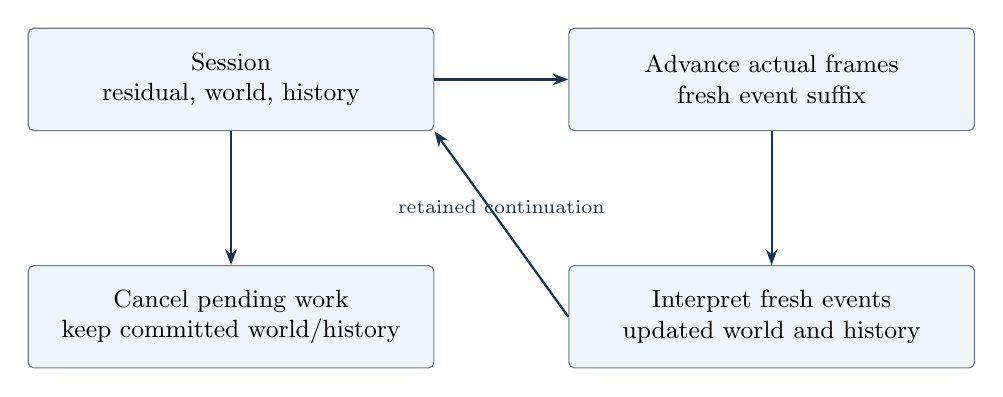
\begin{tikzpicture}
  \node[wide] (session) {Session\\residual, world, history};
  \node[wide,right=17mm of session] (advance) {Advance actual frames\\fresh event suffix};
  \node[wide,below=17mm of advance] (commit) {Interpret fresh events\\updated world and history};
  \node[wide,below=17mm of session] (cancel) {Cancel pending work\\keep committed world/history};
  \draw[arr] (session) -- (advance); \draw[arr] (advance) -- (commit);
  \draw[arr] (commit.west) -- node[hint,above]{retained continuation} (session.south east);
  \draw[arr] (session) -- (cancel);
\end{tikzpicture}
\end{center}

The independent recursive \name{Runs} relation supplies the meaning of
children and caller continuations. Explicit frames realize that meaning with
the exact ordered trace. \name{Session.resume_add} gives the complete sliced
state law. \name{Session.cancel} discards pending execution and preserves
the committed world/history; later resumes stutter.

Pairwise commuting actions permit a permutation theorem for the final world.
The ordered trace still records a different schedule. A negative control
shows a reversed noncommuting pair changes the world. Commutation must be
proved for the actual actions and interference conditions.

The general event machine also has resumable service handling. A request can
run another machine while retaining the caller and service continuations;
faults, stuck endpoints and divergence remain distinct from replies. This is
related to the handler-as-computation approach of interaction trees~\cite{ITrees};
the present interface uses explicit states and finite budgets.

\subsection*{First-order configurations in the shared scheduler}

\name{ProductiveCoreAdapters.EventCursor} connects an event machine to the
existing indexed cursor protocol. Its retained client control is an event
history paired with the machine's existing outcome; a provider inspection
executes exactly the declared machine transition. The adapter introduces no
host closure or additional program syntax. \name{advance\_run} preserves the
whole finite run and its declared transition account, and
\name{advance\_exhausted} identifies every live cut with its actual paused
packet. An unbounded execution remains live at every scheduling allowance.
Terminal client bookkeeping cannot answer a machine request or turn it into
successful completion.

The PeTTa \name{Scoped.Scheduler} instance retains the actual allocator,
choice delimiters, bindings, collection scopes, callers and reached world.
\name{visit\_source\_iff} and \name{resumed\_source\_iff} compare the real
cursor execution with independent source derivations in both directions.
\name{resume\_source\_cut} continues the exact source residual and appends
only its later publications. The source delimiter counterexample remains
observable through this adapter. These laws use the saved world; changing
that world, consuming publication authority or licensing external cancellation
still requires the corresponding interaction contract. Transition accounts
do not bound time spent inside a primitive.

The checked HE worker uses the same first-order adapter with its complete
configuration and an explicit type-lookup policy. Its scheduling split retains
the reached cursor and account. A separate depth grant replenishes only the
saved evaluation or leaf operation, preserving prior publications and the
selected lookup policy. It leaves primitive-service requests unchanged.
The controls begin at a real zero-depth request: scoped lookup then keeps two
polymorphic calls independent, whereas literal lookup retains its type conflict.
This worker/protocol connection is distinct from proving the remaining general
scoped source correspondence and from granting external effect authority.

The downstream \name{RecursiveService.CheckedAdmission} instance checks
currentness before advancing this read-only worker. It uses the existing
ordered dependency store and indexed authority: the captured read stamp must
validate in the current store, and the current right must admit the required
frame-preserving update. Along the store's actual update history, validation
preserves the complete ordered space query, including absence and duplicates.
An invariant of actual checked transitions identifies that query with the
saved worker's space. Equal counters in unrelated stores do not establish
this fact.

\name{resume\_reached\_cut} and \name{resume\_reached\_depth} preserve
the actual suffix, old publications and transition account under the same
type policy. A denied entrance retains the complete paid cursor. Explicit
depth grants are checked at this same boundary; an external primitive request
remains unserved. \name{scoped\_source\_resume\_completed} additionally
joins the independently proved covered source family with closed type
annotations. Its result is the exact source result history and terminal
configuration. Schematic annotations retain their separate correspondence
obligation. This is admission under a supplied current world and right,
not authority consumption, external cancellation, atomic publication or a
native concurrency theorem.

\subsection*{Owned interaction}
The pure session and cursor laws do not enforce exclusive ownership: copying an
earlier cursor can redeliver, and restarting a program can repeat an increment.
The owned host adds consuming authority. A retained computation begins under a
ticket; submitting its derived actions consumes the ticket, applies the actions
once to the shared world and issues the successor ticket. A used ticket is refused
(\name{Owned.used_ticket_refused}), so copies of a computation act at most once
(\name{Owned.copies_act_once}); a cancelled computation refuses further work,
private forks never touch the shared world, and every reached host state accounts
its world as the initial world under the delivered actions. For commuting actions
the final world does not depend on the interleaving (\name{interpret_commute_past},
\name{interpret_interleaving}); a noncommuting pair is a negative control.
External crash recovery, durable exactly-once delivery and the disposition of
non-droppable obligations need a service protocol beyond this sequential host.

\sources{\name{Mettapedia/Machines/OwnedPullDriver.lean},
\name{Mettapedia/Machines/ExecutionHistoryReadout.lean},
\name{Mettapedia/Machines/ResourceOwnership.lean},
\name{Mettapedia/Machines/ProductiveCoreAdapters.lean},
\name{Mettapedia/Languages/MeTTa/HE/FirstSuccessRecursiveExecution.lean},
\name{Mettapedia/Languages/MeTTa/PeTTa/EagerDFSStreaming.lean},
\name{Mettapedia/GSLT/Distinction/ProductiveBlocks.lean}.}

\newpage
\section{The fixed C-language machine}

The fixed core is a source language over the existing C11 semantic modules:
typed integer operations under a selected integer model and signed-conversion
policy, byte memory with effective types, automatic object scopes and array
pointers. Names resolve through the lexical scopes of the current activation.
Pure expressions read integer elements, compute, take addresses and move pointers
within live arrays. Statements assign through places, set pointer variables, call
functions recursively with parameter objects, return values, branch, loop, break
and continue, open blocks that reserve declared objects and retire every owned
lifetime on every exit, allocate and release dynamic objects, and suspend on
external requests.

\begin{center}
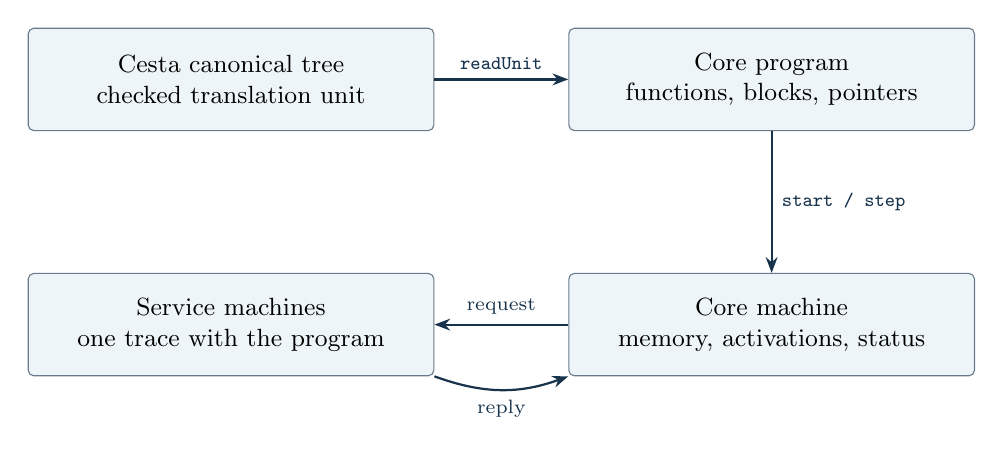
\begin{tikzpicture}
  \node[wide] (ast) {Cesta canonical tree\\checked translation unit};
  \node[wide,right=17mm of ast] (core) {Core program\\functions, blocks, pointers};
  \node[wide,below=18mm of core] (machine) {Core machine\\memory, activations, status};
  \node[wide,below=18mm of ast] (service) {Service machines\\one trace with the program};
  \draw[arr] (ast) -- node[hint,above]{\texttt{readUnit}} (core);
  \draw[arr] (core) -- node[hint,right]{\texttt{start / step}} (machine);
  \draw[arr] (machine.west) -- node[hint,above]{request} (service.east);
  \draw[arr] (service.south east) to[out=-20,in=-160] node[hint,below]{reply} (machine.south west);
\end{tikzpicture}
\end{center}

The executable step is sound and complete for an independent step relation whose
premises are the memory, scope and expression judgments (\name{step_iff}), up to the
two choices C11 leaves open: the identity of each new object and whether an
allocation succeeds. Undefined behaviors stop with their reason: arithmetic
overflow or division by zero, an access to a dead, indeterminate, out-of-bounds or
misaligned element, a trap representation, a pointer formed outside its array, an
invalid or repeated release, or a used missing return. A constraint violation and
a failed host service are reported separately.

The common \name{FixedCore.machine} selects the canonical fresh-identity,
successful-allocation policy. The choice-complete \name{FixedCore.Scheduled}
instance instead retains a C configuration and a finite tape of permitted
choices. Every finite independent source path constructs such a tape;
\name{source_path_iff} proves preservation and reflection with the complete
represented endpoint. One choice is consumed per C step, so repeated visits
to the same C state may make different choices. Each step publishes its actual
configuration pair. Exhausted prefixes retain exactly the unused tape and
the corresponding source path; an empty tape requests replenishment without
reporting C failure. A supplied invalid identity is distinct from source
undefined behavior. External service requests retain their own request kind,
and replies preserve the tape. \name{finished_source_iff} relates completed
results to finite source paths, while \name{resume_with_supply} appends future
choices without replaying committed steps.

The Cesta reader is a static checker for the core fragment. Names resolve through
the C block scopes, operands are integers or pointers to a declared integer type,
and calls are checked against the signatures of the program's functions and of the
host's services. Interleaved declarations become nested blocks; \code{E1[E2]},
\code{&*E} and \code{&E1[E2]} follow their C11 equivalences; returned values and
service arguments are converted to the declared types; the end of \code{int main}
returns \code{0}. Every reading function is equivalent to an independent reading
relation (\name{readUnit_iff}). Constructs outside the fragment are refused, not
approximated. Sources parsed by the Cesta binary run on the core to the values GCC
and Clang compute. On the undefined controls, AddressSanitizer and
UndefinedBehaviorSanitizer report the use after scope, use after release, double
release and overflow under both compilers; only Clang reports the pointer formed
past its array.

Requests are served by service machines through the common callback protocol
(\name{served_call}); running services as machines is a compilation stage from
atomic answers (\name{servedStage}). With the retained HE evaluator as the service,
a C loop calling a MeTTa function returns what GCC computes for the same loop over a
C definition, and the trace contains exactly the evaluator's result occurrences
(\name{metta_call_publishes_evaluator_meaning}). Several results, or an unreadable
one, stop the program with the service's fault: a reply never selects one result
from several.

The scoped service also has an independent source connection.
\name{checked_service_source_completed} constructs completion from an
admitted \name{AtomDerivation} and its local operation coverage; it does not
assume an already completed evaluator run. The transfer profile has closed
type annotations, while equation instances and caller bindings may remain
open. Its events are exactly the source occurrences, and its reply is
determined by the complete batch. Publication of the final occurrence alone
is still an exhausted configuration, rather than a completed reply.

\name{scoped_metta_call_source} lifts this law through the actual C call and
request codec. \name{scoped_metta_resume_source} keeps the waiting C caller
attached to the saved HE configuration and executes only its remaining
events before returning one reply. The saved prefix and the suffix partition
the original source batch. A loop control returns nine through this scoped
service; the two-answer control reports the service fault instead of
selecting an alternative. These are formal machine and callback laws, not
verification of a compiled CeTTa binary or of unrestricted schematic types.

The located layer remains the place for side effects inside expressions. Its
expression scheduling makes full-expression boundaries and unsequenced conflicts
explicit, and \name{StatementExecution.execute_iff} connects its executable
transition to independent rules.

The common fixed/located fragment now has a constructed translation. An
executable lowering agrees with an independent admission relation for arbitrary
finite pure expressions and for assignment, conditionals, loops, break,
continue and return. Pure expression schedules preserve the same scalar and
semantic memory. An assignment additionally executes its actual conversion,
store and returned-value occurrences. Both legal store/result orders reach
the same boundary; neither may bypass an unfinished operand.

\name{statement_step_simulation} and \name{control_step_simulation} replace
one fixed-core control step by its actual located expression and boundary
steps. Their finite-history composition covers arbitrary admitted successful
runs. \name{Block.finished_realization} then executes the final verdict on the
existing budgeted runner and retains the complete receipt list and unused
schedule suffix. The common memory relation preserves object allocation and
lifetime headers as well as contents; reads outside their admitted live
catalogue are refused. A counter loop reaches zero with the committed values
$[2,1,0]$ under both store/result policies.

Different legal evaluation orders can encounter different first faults when
both pure operands fail. The cross-layer observer therefore distinguishes a
defined scalar result from failure without identifying those diagnostics.
Each located execution retains its own exact fault and chronological prefix.
The whole-run reverse construction now discovers the owning source control
through every partial expression and assignment history. Its
\name{ReachedControl.step} either constructs a genuine source step or strictly
decreases finite pending-expression work. Thus arbitrary source loops remain
possible while an infinite stretch of source-free administration is excluded.
\name{terminal_observation_iff} proves preservation and reflection of complete
success or refusal under the admitted scheduler. The schedule license checks
the actual next ready occurrence; an unready operation is malformed scheduling,
not source undefined behavior. \name{ReachedControl.run} additionally retains
the earned source prefix and exact receipts at every budget exhaustion and
selection request. No supplied decomposition into source blocks is required.

\sources{\name{Mettapedia/Languages/C11/FixedCore.lean},
\name{Mettapedia/Languages/C11/FixedCoreStatements.lean},
\name{Mettapedia/Languages/C11/CestaFixedCore.lean},
\name{Mettapedia/Languages/C11/FixedCoreServices.lean},
\name{Mettapedia/Languages/MeTTa/HE/RecursiveService.lean},
\name{Mettapedia/Languages/C11/LocatedStatements.lean},
\name{Mettapedia/Languages/C11/StatementExecution.lean},
\name{Mettapedia/Languages/C11/ExpressionEventHistory.lean},
\name{Mettapedia/Languages/C11/StatementMachineRefinement.lean}.}
\scope{Object layouts are the selected ABI's, an explicit parameter; pointer
variables hold an abstract provenance-carrying value; external services answer each
request at most once. Named extensions outside the core include calls inside
expressions, pointer-typed objects in byte memory, structures, floating types,
\code{for}, \code{do}, \code{switch} and \code{goto}, array initializers, function
pointers and threads. The common-fragment translation does not additionally
cover calls, allocation instructions or side-effecting operands. These remain
available only at their separately specified machine boundaries.}

\newpage
\section{Regional machines and explicit crossings}

A useful machine comparison fixes three things: a region of admitted programs,
the observations to preserve, and the resource objective. Removing an
observation can permit more representations, but does not by itself establish
a faster implementation. Operational accounts and measured native costs are
different claims.

\begin{center}
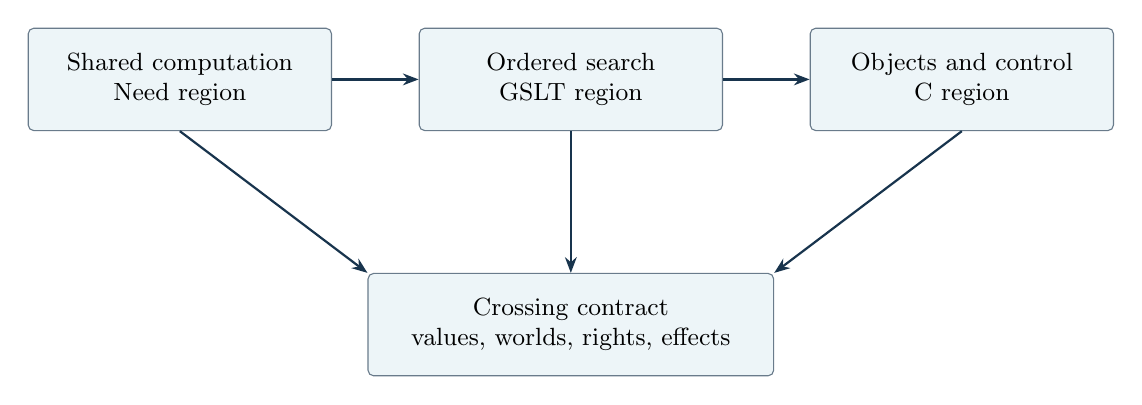
\begin{tikzpicture}
  \node[box] (need) {Shared computation\\Need region};
  \node[box,right=11mm of need] (search) {Ordered search\\GSLT region};
  \node[box,right=11mm of search] (c) {Objects and control\\C region};
  \node[wide,below=18mm of search] (contract) {Crossing contract\\values, worlds, rights, effects};
  \draw[arr] (need) -- (search); \draw[arr] (search) -- (c);
  \draw[arr] (need.south) -- (contract.north west);
  \draw[arr] (search) -- (contract);
  \draw[arr] (c.south) -- (contract.north east);
\end{tikzpicture}
\end{center}

A crossing states what is translated, which observer is preserved, what
dependency/authority evidence travels, and how return or refusal behaves.
Pairwise agreement is insufficient for arbitrary networks: composed paths
must satisfy the applicable compatibility laws. Existing gluing results cover
equation models over a shared binding algebra, equivalence-valued view systems
with trivial cycle transport, and compatible causal histories with explicit
read/write and observation hazards. None of these identifies arbitrary guest
logics or supplies their complete native execution. A general sheaf account of
regional machines still needs its actual restriction and gluing maps.
Trivial cycle transport concerns changes of view that claim to preserve the
same object. An effectful computation cycle can change the world and emit
events; it is not such an identity transport.

\subsection*{Observation, demand and retention are separate controls}
An observer chooses what distinctions a user sees. Demand chooses how much
work is requested. Retention chooses what remains available for inspection or
continuation. \code{once} and \code{select k} bound requested successful
occurrences; they are not general permission to erase faults, reorder effects
or discard owned pending work. Zooming out can license a coarser readout;
zooming in later is possible only if the required information was retained.

\subsection*{Machines do not impose one universal logic}
Conversion within one shared logic and transport between distinct logical
guests have different contracts. A selected machine family retains each
kernel's own state and question type. It does not make HOL, dependent type
theory and set theory one calculus. A stable guest can remain stable while
Prime's candidate develops, provided the crossings state their assumptions.

ZINC~\cite{ZINC} is useful historical comparison for an ML implementation.
Here ZAM denotes a \emph{zipper abstract machine}, which is a different idea
and is discussed in Section~\ref{sec:holes}. No general WAM optimality theorem
is claimed. New regional machines can be
derived or compared through these interfaces, then judged by correspondence
and an explicit cost model.

\scope{The integration target is faithful higher-order MeTTa execution.
CAM and the fixed C core supply substantial instances and reusable laws;
they do not displace that language-facing purpose.}

\newpage
\subsection{Modules, presentations and necessary machine state}

A module assembles declarations and their selected policy layers. A GSLT
states their operational meaning. A regional machine realizes that meaning
with its own representation and control. These are distinct objects: joining
declarations neither selects an evaluation strategy nor proves that two
machines can interact safely.

Universality and the absence of a globally best optimizer do not determine
how many machine families an implementation must expose. One interpreter can
itself dispatch among several strategies. Regional specialization is justified
by a stated program region, correspondence and resource objective, rather
than inferred from undecidability alone.

A region can support a portfolio of implementations, including difficult
higher-order regions; it need not have one fixed algorithm. Vampire provides
an operational precedent for scheduling configurable proof strategies from
workload features~\cite{DynamicStrategyPriority}. The existing bounded-search
portfolio retains private batches, distinguishes cutoff from exhaustion and
publishes one strategy's batch. Combining strategies' rediscovered answers
would require a separate occurrence correspondence. Fair scheduling alone
does not certify exhaustion after a finite budget.

Constraint-solving backends are also candidates for finite collection
matching. A checked encoding must relate decoded solutions to the declared
source matches, preserving their occurrence identities. Auxiliary Boolean
assignments need not correspond one-to-one with those matches, so ordinary
model counting does not automatically count semantic answers. SAT witnesses
and checked unsatisfiability certificates can justify different conclusions;
the encoding and coverage obligations remain~\cite{LRAT}. Specialized AC
representations can also be effective for important restricted rule
classes~\cite{EkerAC}. The general complexity bound does not choose the best
implementation for a workload.

\begin{center}
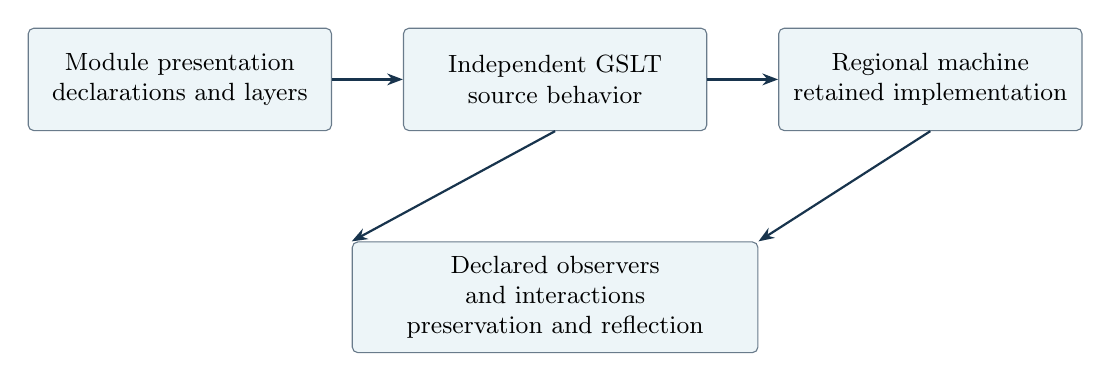
\begin{tikzpicture}
  \node[box] (module) {Module presentation\\declarations and layers};
  \node[box,right=9mm of module] (gslt) {Independent GSLT\\source behavior};
  \node[box,right=9mm of gslt] (machine) {Regional machine\\retained implementation};
  \draw[arr] (module) -- (gslt);
  \draw[arr] (gslt) -- (machine);
  \node[wide,below=14mm of gslt] (observer) {Declared observers and interactions\\preservation and reflection};
  \draw[arr] (gslt.south) -- (observer.north west);
  \draw[arr] (machine.south) -- (observer.north east);
\end{tikzpicture}
\end{center}

An admitted execution region restricts a backend's qualification, not the
module format. A first-order backend can refuse a presentation containing
binders while retaining that presentation for a suitable scoped interpreter.
A general interpretation path and its specialized realizations should share
an independent source observation; the existence of that path does not by
itself establish coverage of every binder or premise form.

The presentation and its surface syntax also have different responsibilities.
The existing five-field \name{LanguageDef} carries sorts, constructors,
equations and rewrites; \name{ExtendedLanguageDef} attaches independently
authored dependent layers. A proof calculus is one such layer. Several concrete
syntaxes can elaborate to this shared structure. Upstream syntax is an
interchange route, not a requirement that every local extension fit a
historical grammar. Improvements to notation must preserve binding, declaration
origins and the laws of the selected layers.

Four current boundaries must not be conflated: the closed-theory
\name{moduleTheory!} Lean quotation; the structured \name{module/1} envelope;
textual \name{.module} languages; and the live runner's emitted MeTTa program.
The quotation and envelope already have structural elaboration laws. The
runner's \name{ReadAfterRender} theorem concerns MeTTa program text, not the
upstream module grammar. Exact program-text rendering excludes the anonymous
variable marker as a literal variable name, since the reader allocates a
fresh occurrence there; the underscore symbol remains ordinary data.
A canonical portable surface now establishes
\[
  \mathsf{readBytes}\bigl(\mathsf{renderBytes}(P)\bigr)
    =\mathsf{some}(P),
\]
with a separate elaboration theorem into the existing assembled presentation.
The character reader uses the existing lexer/parser/atom-reader pipeline;
the byte reader validates UTF-8. The complete finite \name{LanguageDef}
codec retains binders, collection metadata, equations and scoped premises.
Dependent layers carry an explicit indexed codec; proof calculi, export
names and products are concrete instances. This does not claim that every
Lean function or relation has a finite serialization.

The surface is an inert \code{(module:document payload)} declaration.
Origin-bearing entries survive the text boundary before the existing import
contract decides sharing or collision. Unknown envelope payloads remain data;
a declared layer rejects an incompatible schema. The canonical syntax does
not implement a historical upstream grammar. Preserving comments, formatting
and import expressions still requires a separate source representation:
an assembled presentation cannot reconstruct information it has discarded.

A finite rule list need not imply first-order syntax: its rules can have
binders and higher-order premises. An effectively enumerable rule family
additionally needs a finite generator description and evidence for each
selected instance. An arbitrary semantic relation in Lean's abstract
\name{GSLT} record need not be effectively enumerable or serializable.
Keeping that semantic generality is compatible with requiring explicit
presentation and realization evidence at an executable boundary.

Even a simple specialization must carry the typing boundary. A variable-root
rule $x:\mathsf{Nat}\rightsquigarrow\mathsf{zero}$ structurally matches a
Boolean term if its type is forgotten. Checked invocation-sort selection must
exclude that candidate before execution, retaining the original indices of
later rules. Comparing two untyped implementations would miss this error.
The same contract must fix when query inputs become available. In the checked
provider profile considered here, an output of the current query does not
retroactively satisfy a required input to that query.

The question of necessary state is relative to the admitted observations and
future interactions. Write
\[
 s\approx_{O,\mathcal C}t
 \quad\Longleftrightarrow\quad
 \forall C\in\mathcal C,\quad O(C[s])=O(C[t]).
\]
The observation may include outcomes, residuals, effects or probability laws.
An encoding supporting every such interaction cannot identify states outside
this equivalence. Turning it into a machine quotient additionally requires
stability under the actual transitions and contexts. This identifies necessary
distinctions, not a fastest implementation or a computable finite quotient.

The contextual observed-coalgebra owner constructs a quotient, its transition
square and exact factorization for compatible natural consumers. That owner
uses labelled set-valued futures: order, multiplicity and probability require
their additional representations and laws. Its quotient is not already the
complete MeTTa machine. The ordered-machine bridge also reads an ordered
successor list as a GSLT membership relation; that modal view alone forgets
list order and repeated successors.
Occurrence simulations transport these ordinary modal formulas without a
positional alignment. The converse fails for occurrence preservation: a
one-successor machine and a machine with two equal successor occurrences
satisfy the same formulas, while their occurrence bags have different
cardinality. This limitation is proved in the native-type bridge.

\begin{center}\small
\begin{tabularx}{\textwidth}{@{}>{\raggedright\arraybackslash}p{36mm}
  >{\raggedright\arraybackslash}X>{\raggedright\arraybackslash}X@{}}
\toprule
Admitted region & Useful machine structure & Distinction to preserve\\
\midrule
Functional terms & CEK, Krivine, CAM or Need & Strategy, captured environment, shared demand\\
Rule search & Retained matcher and frontier & Occurrence identities, selected traversal, residual work\\
Reflective processes & Communication/reaction machine & Names, quotation, ports, permitted scheduling\\
Certificate checking & Decoder, proof state and snapshot & Declared theory, references, checked evidence\\
Probabilistic programs & Kernel-valued machine and history & Draw identity, scores, captured random values\\
\bottomrule
\end{tabularx}\end{center}

Algebraic operational semantics connects syntax and behavior through a
distributive law when the required rule-format and categorical hypotheses
hold~\cite{TuriPlotkin}. Polynomial syntax alone does not provide that law.
Likewise, module-join compatibility is distinct from preservation of conversion
or effects. The existing first-match priority counterexample fails substitution
stability; ordinary relational rewriting has its own substitution theorem.

\sources{\name{Mettapedia/GSLT/LanguageDef/ModuleAlgebra/Semantics.lean},
\name{Mettapedia/GSLT/LanguageDef/ExtendedLanguageDef.lean},
\name{Mettapedia/GSLT/LanguageDef/ModuleAlgebra/UpstreamTheoryQuotation.lean},
\name{Mettapedia/GSLT/LanguageDef/ModuleFormat/Authoring.lean},
\name{Mettapedia/GSLT/LanguageDef/ModuleFormat/Text.lean},
\name{Mettapedia/GSLT/LanguageDef/ModuleFormat/Portable.lean},
\name{Mettapedia/Languages/MeTTa/PeTTa/Bridges/MeTTaIL/GeneralLiveRunnerEmission.lean},
\name{Mettapedia/Machines/BoundedSearchPortfolio.lean},
\name{Mettapedia/GSLT/Logic/ContextualObservedCoalgebraQuotient.lean},
\name{Mettapedia/OSLF/Framework/OrderedSystemNativeTypes.lean},
\name{Mettapedia/GSLT/Dedukti/LeanMinusPriority.lean}.}

\newpage
\subsection{Staged lowering and runtime interaction}

There are two different ways for one language machine to use another.
\emph{Staged lowering} transforms the source before execution.
\emph{Runtime interaction} keeps both computations alive across requests and
returns. Both need semantic preservation, but they retain different states.
Operational semantics based on explicit language boundaries is established
work~\cite{MultiLanguage}; hygienic macro binding also has its own semantic
models~\cite{ScopeSets}.

\begin{center}
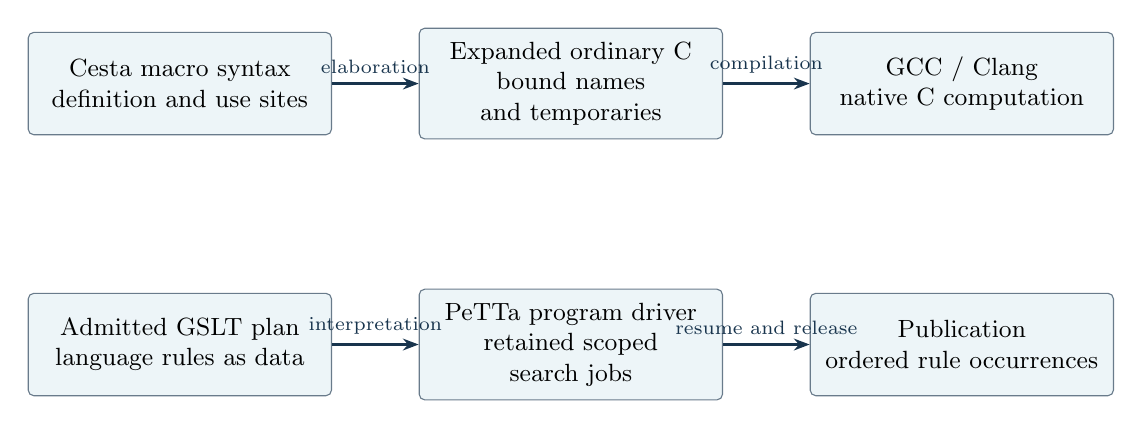
\begin{tikzpicture}
  \node[box] (macro) {Cesta macro syntax\\definition and use sites};
  \node[box,right=11mm of macro] (expanded) {Expanded ordinary C\\bound names and temporaries};
  \node[box,right=11mm of expanded] (native) {GCC / Clang\\native C computation};
  \draw[arr] (macro) -- node[hint,above]{elaboration} (expanded);
  \draw[arr] (expanded) -- node[hint,above]{compilation} (native);
  \node[box,below=20mm of macro] (presentation) {Admitted GSLT plan\\language rules as data};
  \node[box,right=11mm of presentation] (jobs) {PeTTa program driver\\retained scoped search jobs};
  \node[box,right=11mm of jobs] (receipts) {Publication\\ordered rule occurrences};
  \draw[arr] (presentation) -- node[hint,above]{interpretation} (jobs);
  \draw[arr] (jobs) -- node[hint,above]{resume and release} (receipts);
\end{tikzpicture}
\end{center}

Cesta's current macro engine instantiates templates, resolves explicit binding
origins, introduces fresh locals, and emits C. Argument metadata distinguishes
syntax, values and modifiable places, with evaluation contracts. For the
checked narrowing library, source and target types are syntax; the input value
and output place are evaluated once by the emitted C. Macro expansion does not
execute the input expression. The native compiler supplies active-header name
inventory and checks the final C. This is a staged language layer; it is not an
extra interpreter running beside the resulting native program.

The current GSLT driver instead retains a licensed request and actual search
state for every job. Requests carry the presentation/environment, permissions,
binding context, expected type, source and physical rule/site identity.
Receipts retain matcher choices, captured and completed assignments, premise
history, and local and reconstructed targets. The quoted authored equations
are connected to PeTTa evaluation. The general target-step theorem requires
an equation-free, checked-stratified plan and sufficient search allowance.
Its exact canonical reduct-list theorem has a narrower root query-profile
scope. A presentation emitter and a general whole-run loop still need their
complete integrated proofs.

Treating an expander as an abstract machine can clarify its own binding and
phase semantics. It does not require paying for that machine at program runtime:
justified lowering can remove it. A live heterogeneous computation needs
runtime crossing rules in addition to staged source transformations.

\sources{\name{Mettapedia/GSLT/LanguageDef/MacroTemplateNames.lean},
\name{Mettapedia/GSLT/LanguageDef/MacroDefinitionPorts.lean},
\name{Mettapedia/GSLT/LanguageDef/MacroCheckedNarrowing.lean},
\name{Mettapedia/Languages/MeTTa/PeTTa/Bridges/MeTTaIL/GeneralProgramDriverExecution.lean}.}

\newpage
\subsection{A computational-metagraph machine as a candidate}

A candidate Meta-MeTTa machine would retain regional computations at nodes
and pending crossings at edges. Admission, transfer, advancement, reply,
refusal, cancellation and dependency validation would be explicit steps.
This heterogeneous machine remains an integration target.

\begin{center}
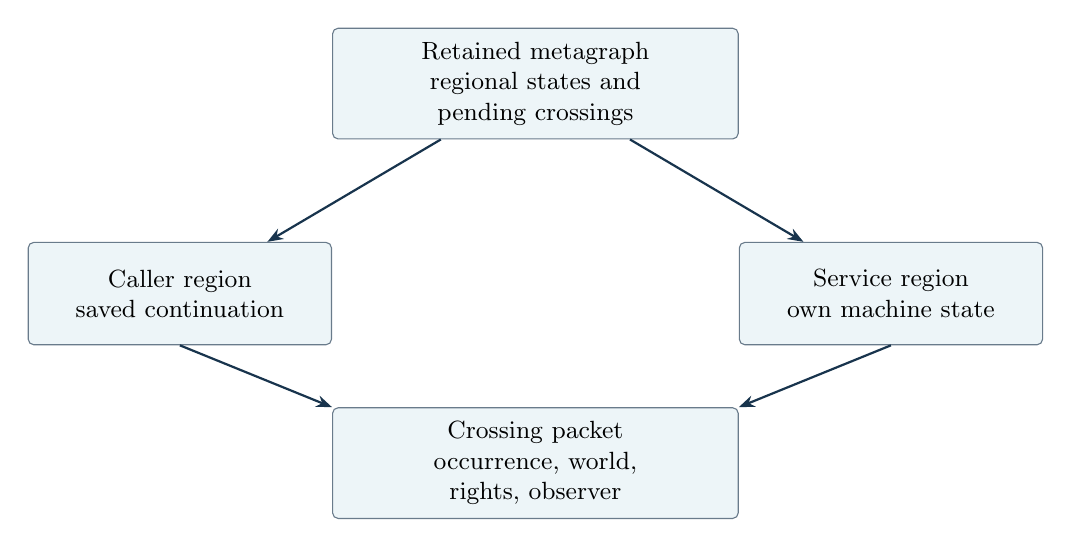
\begin{tikzpicture}
  \node[wide] (graph) {Retained metagraph\\regional states and pending crossings};
  \node[box,below left=13mm and 0mm of graph] (caller) {Caller region\\saved continuation};
  \node[box,below right=13mm and 0mm of graph] (service) {Service region\\own machine state};
  \node[wide,below=12mm of graph,yshift=-22mm] (edge) {Crossing packet\\occurrence, world, rights, observer};
  \draw[arr] (graph) -- (caller); \draw[arr] (graph) -- (service);
  \draw[arr] (caller.south) -- (edge.north west);
  \draw[arr] (service.south) -- (edge.north east);
\end{tikzpicture}
\end{center}

The state needs continuations, ordered occurrences, dependency evidence,
consuming authority and committed history. Each crossing must realize an
independent semantics preserving the selected observations.

\name{MachineCore.familyCore} retains heterogeneous state/question types but
cannot change the selection. \name{Machine.handle} constructs interaction
with retained caller and service states. \name{ScheduledFrontier} preserves
occurrence slots across differing completion times, under independence
hypotheses. Publication, read-validation and effect-session laws still need
the common ownership join.

\name{GSLT.Poly.BindingSignature} represents binding terms as a context-indexed
free monad. The indexed polynomial client in \name{GSLT.Poly.SortedTraversal}
retains argument occurrences and reply slots. Neither polynomial structure nor
a slot determines a child's interpretation or force rights.

In the MM2 evidence-material theory, two actual matcher paths conclude the
same fact but deliver different origin lists. Their consuming continuation
cannot factor through conclusion support. An ordered material batch or receipt
retains enough information; the recovery theorem uses a classical partial
inverse, rather than an executable native decoder.

Native MM2 controls separately run a finite staged consumer on three input
occurrences, two with equal payloads. Shared choice gives six deliveries;
separate choice coordinates give twelve. Sequence fields recover their order.
Retained cursors preserve the answers and three counter updates across reloads.
Restarting repeats an update; changing the captured environment changes later
answers. \code{head 1} alone still permits sibling writes. This does not
establish a general MeTTa correspondence or external-effects protocol.

Producer identity supports sharing; delivery identity supports occurrence
observation. Indexed set storage can retain both views. The richer encoding
then carries the surrounding machine's cursor, world and commitment protocol.

\sources{\name{Mettapedia/Machines/MachineSubstrate.lean},
\name{Mettapedia/GSLT/Distinction/ProductiveBlocks.lean},
\name{Mettapedia/GSLT/Distinction/OrderedSimulationSpans.lean},
\name{Mettapedia/GSLT/Distinction/CausalGluing.lean},
\name{Mettapedia/GSLT/Scope/Holonomy.lean},
\name{Mettapedia/GSLT/LanguageDef/ModuleAlgebra/SemanticGluing.lean},
\name{Mettapedia/GSLT/Poly/SortedTraversal.lean},
\name{Mettapedia/GSLT/Logic/ProgrammableSpaceMM2EvidenceMaterial.lean}.}

\newpage
\subsection{The trinity as a fibred web of presentations}

The language-facing trinity names intensional mathematics, extensional
mathematics and a GSLT-IL operation presentation. These are semantic roles,
not necessarily separate kernels. The contextual computational-trinity
framework compares programs, proofs or typed terms, and generalized elements
in spaces. Each face is a presheaf over contexts, so substitution is part of
the presentation rather than an untracked surrounding operation.

\begin{center}
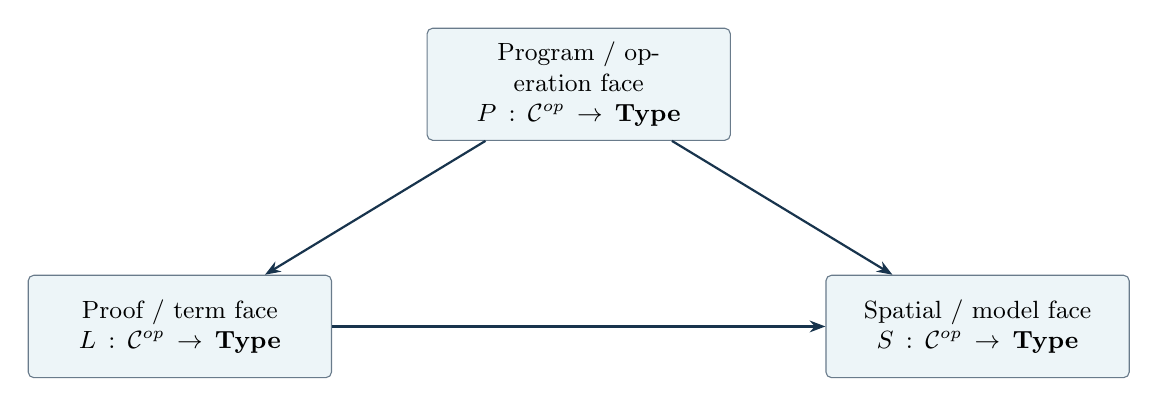
\begin{tikzpicture}
  \node[box] (program) {Program / operation face\\$P:\mathcal C^{op}\to\mathbf{Type}$};
  \node[box,below left=17mm and 12mm of program] (logic) {Proof / term face\\$L:\mathcal C^{op}\to\mathbf{Type}$};
  \node[box,below right=17mm and 12mm of program] (space) {Spatial / model face\\$S:\mathcal C^{op}\to\mathbf{Type}$};
  \draw[arr] (program) -- (logic);
  \draw[arr] (program) -- (space);
  \draw[arr] (logic) -- (space);
\end{tikzpicture}
\end{center}
\diagramcaption{Comparison means a commuting triangle of natural maps.
Exactness additionally requires invertible maps. The abstract construction
does not instantiate the whole native DTT/HOL/set/GSLT triangle.}

Actual categorical owners already have different variances. Theory models
reindex by reducts along theory arrows, forming a Grothendieck fibration.
Typed open code has forward transport and cocartesian lifts. Finite retained
execution paths form another category-valued index. These constructions do
not make every theory arrow an executable, resource-safe or conservative
machine crossing. The complete step, residual and observer comparison must
be added for the actual route. The additive world-model doctrine likewise
cannot silently justify deleting a record or normalizing a Bayesian update.

The STT/DTT and selected set-family bridges are scoped interpretations.
Representing a HOL formula does not prove it; a native inhabitant is not
automatically a source HOL derivation. Logical borrowing needs the selected
conservativity contract. Adding a stronger conversion bubble also needs its
own substitution and join laws. Two component normalizers do not necessarily
decide their combined conversion.

Hyperset presentations retain graph occurrences; material equality quotients
by bisimulation. A dependent consumer therefore needs family and section
descent before those distinctions are erased. Internal coalgebraic membership
and the host's well-founded membership remain distinct. Initial/final
comparisons also keep their bounds and existence hypotheses: identifying an
initial algebra with a final well-founded coalgebra does not prove that every
set functor has either~\cite{WellPointed}. Unrestricted powerset has no
set-sized fixed point. Qualified bounded constructions state their size
conditions separately.

\sources{\name{Mettapedia/Computability/ComputationalTrinity.lean},
\name{Mettapedia/GSLT/LanguageDef/TheoryGraphModels.lean},
\name{Mettapedia/Languages/MeTTa/PrimeCandidates/ContextualDataFibration.lean},
\name{Mettapedia/GSLT/Core/OperationalPathFibration.lean},
\name{Mettapedia/TypeTheory/MaterialSets/Hypersets/FamilyDescent.lean},
\name{Mettapedia/Logic/WorldModel/Indexed/Doctrine.lean}.}

\newpage
\section{Proof machines: scoped, licensed composition}
\label{sec:checking}

\begin{quote}
\emph{What follows from what, under which conditions?}
\end{quote}

A checking machine makes a proposed answer to this question inspectable.
The local rules specify the permitted connections; evidence identifies the
connection being proposed; composition connects its output to the next input.
The interface shared by proof checking and rewrite checking is therefore
\emph{scoped, licensed composition}. This identifies a common organization,
while leaving each presentation responsible for its own judgments, equality,
binding and resource rules.

Write
\[
 T;\Gamma\vdash e:A\longrightarrow B
\]
for a supplied piece of evidence $e$ connecting boundaries $A$ and $B$ under
presentation $T$ and scoped conditions $\Gamma$. The notation is schematic:
the boundaries may be premise contexts and conclusions, rewrite states, or
typed interfaces carrying a world and resource obligations. An independent
judgment determines which such connections are licensed. The machine realizes
its checking discipline.

\begin{center}
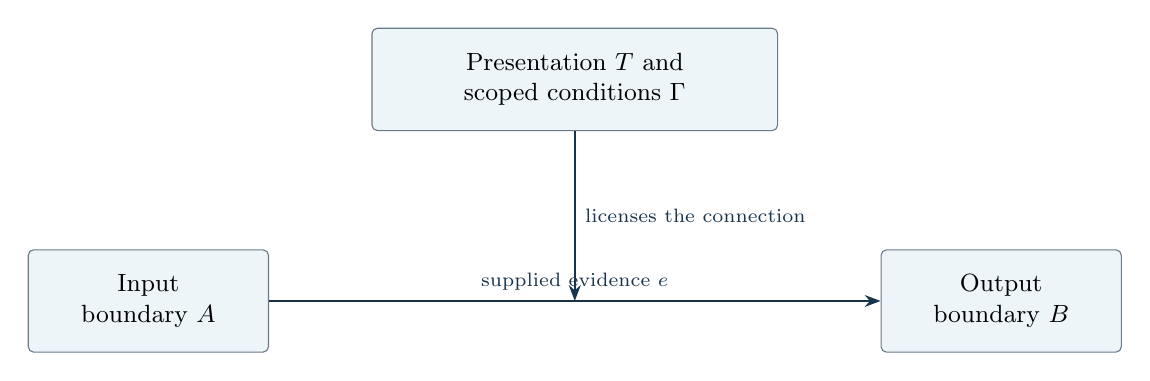
\begin{tikzpicture}
  \node[wide] (conditions) {Presentation $T$ and scoped conditions $\Gamma$};
  \node[smallbox,below left=15mm and 13mm of conditions] (a) {Input\\boundary $A$};
  \node[smallbox,below right=15mm and 13mm of conditions] (b) {Output\\boundary $B$};
  \draw[arr] (a) -- node[hint,above]{supplied evidence $e$} (b);
  \draw[arr] (conditions) -- node[hint,right]{licenses the connection} ($(a)!0.5!(b)$);
\end{tikzpicture}
\end{center}
\diagramcaption{A boundary states what must fit. The selected theory determines
whether evidence is reusable, whether an input must be consumed, and which
conversions are admissible.}

This perspective is continuous with the categorical treatment of proofs and
programs as composable processes~\cite{RosettaStone}, and with rewriting
logic's treatment of computation by proof terms~\cite{RewritingLogic}.
Variable binding requires its own substitution algebra, including weakening,
capture avoidance and metasubstitution~\cite{SecondOrderMetatheory}. These
ingredients explain how a small checker can serve many presentations without
choosing one object logic as their common meaning.

There are distinct categorical levels here. A rule with several premises is
naturally a generator of a multicategory; substitution composes proofs into
its premise slots. A sequence of unary rewrites instead gives paths in a
free category. Exchange, contraction and weakening require the structural
laws of the selected calculus. The category of checking machines describes
realizations of these proof structures, with operational observations and
costs. It is not the proof category itself. This agrees with the nLab's
accounts of deductive systems, multicategories and syntactic
categories~\cite{nLabInference}. Institutions additionally organize signatures,
models and satisfaction under change of notation; they do not by themselves
provide an executable certificate checker.

Storage navigation is a further realization level. A cursor, stack, stream,
tree focus or dependency schedule may organize the same proof evidence.
None is a primitive of every proof calculus. A focused position can be an
observation of a machine---an account of what it is currently attending
to---but a comparison must state whether it preserves that focus or hides
it. Forgetting navigation need not forget the proof's premise dependencies.
The dependency direction is from source rules to checking realizations and
then to storage adapters, rather than from a particular backend to logic.
For the authored-calculus classifying category, closed source derivations
are equivalent to arrows from the empty premise context to a singleton goal;
the two executable maps preserve the actual proof term. VibeITP and Metamath
connect their source judgments at this level, before choosing graph replay
or retained source-address checking.

\subsection{Local evidence, exact checking and coverage}

For one admitted effective presentation, let
$\mathsf{Cert}_T(\Gamma;A,B)$ be the supplied certificate data and let
$\mathsf{Valid}_T(\Gamma;A,e,B)$ be the independent validity judgment. The
local checker earns
\[
 \mathsf{check}_T(\Gamma,A,e,B)=\mathsf{true}
 \quad\Longleftrightarrow\quad
 \mathsf{Valid}_T(\Gamma;A,e,B).
\]
The separate coverage theorem relates this judgment to the intended source
relation:
\[
 A\mathrel{\mathsf{Step}_{T,\Gamma}}B
 \quad\Longleftrightarrow\quad
 \exists e.\;\mathsf{Valid}_T(\Gamma;A,e,B).
\]
The first theorem qualifies the submitted evidence. The second establishes
which source steps have a representation in that evidence language. Neither
asserts that a search procedure will find the evidence within a given budget.
Existential coverage alone also supplies no polynomial-time certificate
translator.

For an ordinary calculus with implication elimination, a local rule is
\[
 \frac{T;\Gamma\vdash p:A\qquad T;\Gamma\vdash q:A\Rightarrow B}
      {T;\Gamma\vdash\mathsf{mp}(p,q):B}.
\]
Its checker resolves the two premise citations, checks the rule instance and
compares the claimed conclusion. A resource-sensitive rule instead states how
its inputs are split or shared. Local computation can instantiate a rule;
evidence must still establish its side conditions. A negative premise such as
``no equation applies'' requires a checked exhaustion argument or a justified
index certificate.

Declaration identity belongs to this boundary. Content addressing can locate
a rule, while exact comparison or stated digest assumptions establish which
rule was found. A repeated declaration can have several occurrences despite
identical content. Certificate references must retain the occurrences required
by the observer. The host additionally identifies the theory it intended to
authorize: a valid proof under a packet's supplied theory does not identify
that theory with an externally requested one.

\subsection{Proof terms, slots and retained ambiguity}

A proof term records enough information to reconstruct the licensed use.
For an authored rewrite this can be a rule occurrence, a typed site, matching
choices, premise references and equation evidence. Deterministic fields can be
computed during replay. The current \name{GeneralRewriteRecipeExpansion}
distinguishes a compact invocation from its expanded firing receipt and proves
sound expansion and reconstruction of valid expanded firings.

Consider a two-input rule $r:(A,A)\to B$ and evidence $p,q$ of $A$.
The terms $r(p,q)$ and $r(q,p)$ record different slot assignments. Their
conclusions may coincide; identifying the derivations requires an explicit
equation or observer. Unique scoped names for slots, together with a
substitution, can encode the assignment. They do not remove choices caused
by collection matching, equations or alternative premise derivations.

Ambiguity may be useful compression. A packed proof structure can retain a
family of alternatives, just as a packed parse forest retains multiple parses.
Its boundary must say whether it certifies one selected derivation, all
represented derivations, or a complete collection of derivation occurrences.
Finding one valid branch licenses an existential claim. Certifying every
represented branch requires their local validity; claiming that the family
contains every source answer additionally requires coverage and multiplicity
laws. Backend traversal order grants none of those permissions.

The following quantities are distinct:
\[
 \text{stored nodes},\qquad \text{reference uses},\qquad
 \text{derivations distinguished by the selected observer}.
\]
A shared node can have many uses. Two positional replay choices can yield the
same firing observation, while two identical declaration copies can generate
distinct answer occurrences. The quotient must name what it forgets and prove
that the remaining consumer descends through it.

Sharing can change certificate size exponentially. A fixed example in
\name{ProofSharingBounds} has an axiom $q_0$ and the rules
$q_n,q_n\vdash q_{n+1}$. Every accepted proof tree of $q_n$ contains exactly
$2^{n+1}-1$ nodes. A chronological DAG instead stores $n+1$ nodes and two
references at each nonbase node. Its checked input size is at most
$4(n+1)^2$ even with unary rule and reference indices. The resulting theorem
excludes every polynomial-size translation from this calculus's DAGs to its
trees. This is a lower bound for the target representation, rather than a
claim about the behavior of one unfolding algorithm. It does not separate
Frege from extended Frege.

Textual parsing is another boundary. A structural certificate reader is not
the lexer and grammar of its source language. Source ambiguity must survive
in the packed parse result until an explicit policy selects, ranks or rejects
it. Binding lowering then preserves the selected scopes. The portable
presentation roundtrip supplies a proved textual surface for its supported
document schema; it does not identify every upstream module grammar with that
surface.

\subsection{The algebra of checked composition}

Five operations expose the common algebra:

\begin{tabularx}{\linewidth}{@{}p{25mm}XX@{}}
\toprule
Operation & Evidence being composed & Required law \\
\midrule
Sequence & $A\xrightarrow{p}B\xrightarrow{q}C$ & Exact joining boundary. \\
Hole filling & Premise outputs into an open derivation & Substitution respects scope and the selected structural rules. \\
Context & A local rewrite inside $C[-]$ & The context is licensed and replacement preserves its typing and binding interface. \\
Sharing & Several references to stored evidence & Every reference use remains justified and counted where required. \\
Parallel & Two orders of independent actions & Checked residual edges close the selected square. \\
\bottomrule
\end{tabularx}

\begin{center}
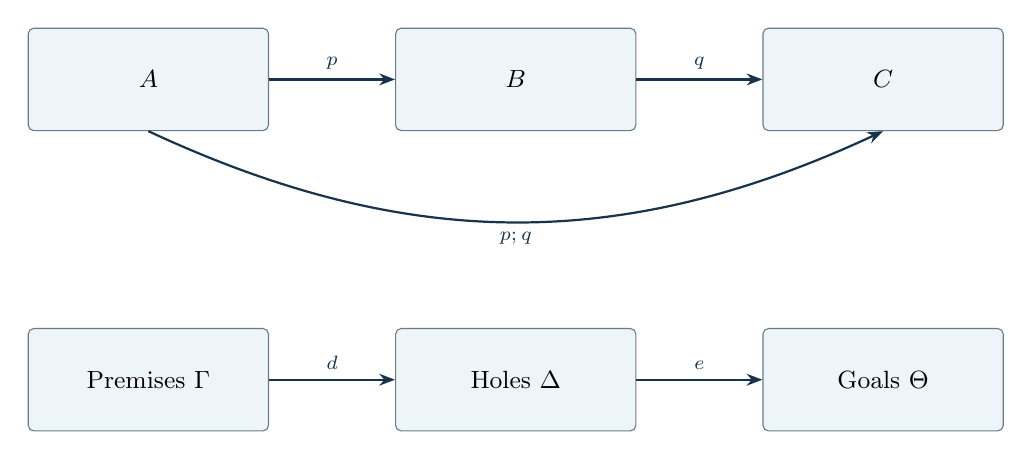
\begin{tikzpicture}
  \node[smallbox] (a) {$A$};
  \node[smallbox,right=16mm of a] (b) {$B$};
  \node[smallbox,right=16mm of b] (c) {$C$};
  \draw[arr] (a) -- node[hint,above]{$p$} (b);
  \draw[arr] (b) -- node[hint,above]{$q$} (c);
  \draw[arr] (a.south) to[bend right=25] node[hint,below]{$p;q$} (c.south);
  \node[smallbox,below=25mm of a] (g) {Premises $\Gamma$};
  \node[smallbox,right=16mm of g] (d) {Holes $\Delta$};
  \node[smallbox,right=16mm of d] (h) {Goals $\Theta$};
  \draw[arr] (g) -- node[hint,above]{$d$} (d);
  \draw[arr] (d) -- node[hint,above]{$e$} (h);
\end{tikzpicture}
\end{center}
\diagramcaption{Temporal composition and premise substitution are distinct
constructions. A particular checker realization relates them by adequacy.}

The common executable law is
\[
 \mathsf{replay}(s,p\mathbin{+\!+}q)
 =\mathsf{replay}(s,p)\mathbin{\gg\!=}
       (\lambda t.\,\mathsf{replay}(t,q)).
\]
It holds for success and refusal in
\name{DerivationGraph.replayFrom_append_eq}; the authored rewrite instance is
\name{GeneralRewriteRecipeComposition.Trace.replay_append}. Its categorical
readout is composition of \emph{partial state transformations}. A bare Boolean
verdict forgets the intermediate state needed for composition. On successful
paths, identity and concatenation give a category of checked executions.

Open derivations have another category:
\name{CertificateGSLTClassifyingCategory} takes premise contexts as objects
and vectors of open derivations as morphisms. Composition substitutes those
vectors into premise holes. Its existing Cartesian structure licenses reuse
and discard. A multi-input or linear presentation needs its corresponding
multicategorical or monoidal structure; these structural permissions are not
consequences of sequencing alone.

The authored checker already realizes the other three operations.
\name{GeneralRewriteRecipeContext} transports local receipts through admitted
typed contexts, including binders.
\name{GeneralRewriteRecipeDAG} admits local recipes and reuses the existing
shared-certificate checker for references and joins.
\name{GeneralRewriteRecipeParallel} checks four original residual firings,
independent addresses, stable site labels and literal endpoint closure; the
accepted square constructs an existing Mazurkiewicz swap. It does not infer
the missing residuals from two disjoint sites. Changed provider worlds or
observable effects require further independence evidence.

\newpage
\subsection{Checking whether another machine was stepped correctly}

Let $M$ have states $S$ and an independently stated transition relation
$s\mathrel{\longrightarrow_M}t$. Suppose local certificates $c$ have earned
the exactness and coverage contracts above. A submitted finite execution is
\[
 s_0\xrightarrow{c_1}s_1\xrightarrow{c_2}\cdots
       \xrightarrow{c_n}s_n.
\]
The checking machine threads the actual state $s_i$ and validates $c_{i+1}$
against the proposed $s_{i+1}$. Induction on the submitted sequence proves
that acceptance is equivalent to validity of all its local certificates.
Coverage then represents every finite $M$-execution. The induction uses the
actual intermediate state, so scope, heap, continuation and world components
cannot be reset between steps.

A checked instruction log is evidence of machine execution; a source evaluation
derivation supplies evidence for the source judgment. Adequacy relates their
claims. One possible result, completed evaluation and a complete result multiset
are different judgments: the latter two require the corresponding terminal or
exhaustive-branching evidence, including duplicate occurrences and pending work.

\begin{center}
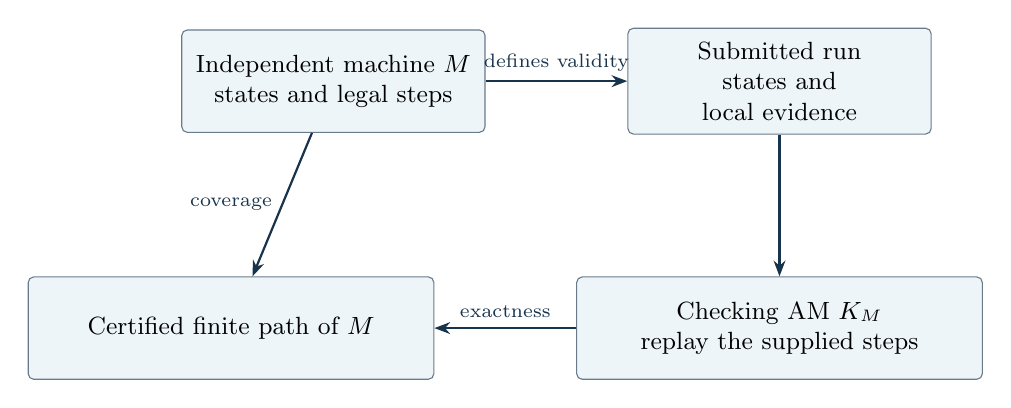
\begin{tikzpicture}
  \node[box] (spec) {Independent machine $M$\\states and legal steps};
  \node[box,right=18mm of spec] (cert) {Submitted run\\states and\\local evidence};
  \node[wide,below=18mm of cert] (checker) {Checking AM $K_M$\\replay the supplied steps};
  \node[wide,left=18mm of checker] (path) {Certified finite path of $M$};
  \draw[arr] (spec) -- node[hint,above]{defines validity} (cert);
  \draw[arr] (cert) -- (checker);
  \draw[arr] (checker) -- node[hint,above]{exactness} (path);
  \draw[arr] (spec) -- node[hint,left]{coverage} (path);
\end{tikzpicture}
\end{center}
\diagramcaption{The checked machine and its checking machine are separate
roles. A machine can play either role once the relevant evidence interface is
constructed. An empty path alone proves neither program formation nor loading
validity.}

This applies to proof-kernel instructions as readily as to CAM instructions,
rho communications or ISA transitions, when their local certificate contracts
are available. The authored GSLT implementation supplies one concrete route:
\name{GeneralRewriteRecipe.check_exact} checks its independent receipt
judgment, and \name{exists_checked_iff_step} covers the original
equation-saturated step relation. Composed recipes reach the existing finite
may-reachability native types. That modal readout establishes the witnessed
finite path; exhaustive search, termination and physical execution cost have
their own obligations.

Checking a run of $K_M$ is another instance of the same pattern. Such reflection
requires an encoding of $K_M$ and adequacy of its transition certificates.
Encoding its states as numbers or graphs preserves only the distinctions
proved for that encoding. It does not turn a certificate about a checker's run
into unconditional soundness of every theory that checker might load.

\subsection{Reconstruction, elaboration and reproducible hints}

A partial reconstructor $r$ can process output from an external prover,
tactic or repair procedure. With destination checker $c$, publication is
\[
 \mathsf{reconstruct}_{c,r}(A,o)=
 r(A,o)\mathbin{\gg\!=}
  \bigl(\lambda p.\;\mathsf{if}\ c(A,p)\ \mathsf{then}\ \mathsf{some}(p)
      \ \mathsf{else}\ \mathsf{none}\bigr).
\]
It returns $p$ exactly when $r$ returned $p$ and $c$ accepted it. No soundness
of the producer is assumed. Producer failure and checker refusal both publish
nothing; the submitted-output coverage theorem states exactly which accepted
certificates the producer can return. Composing two such stages retains both
checking boundaries. This is a general reconstruction interface, not a
completed translation of an arbitrary ATP proof format.

An elaboration has another obligation: an accepted source certificate must
produce accepted destination evidence. Existing local elaborations compose
and lift to articles. Polynomial output size, actual translation time and
logical soundness are separate properties. An output-size bound yields a
size simulation; it does not manufacture an executed polynomial-time
translator. A model interpretation likewise supplies no resource bound.

For reproducible checking, fix a deterministic strategy $f:S\to S$ and an
explicit observation $v:S\to V$ with decidable equality on $V$. A checkpoint
$(k_i,z_i)$ requests $k_i$ strategy ticks followed by the comparison
$v(f^{k_i}(s_i))=z_i$. The checker continues from its \emph{computed} internal
state, never from a replacement state supplied by the certificate. On success,
\[
 s_{\mathrm{final}}=f^{\sum_i k_i}(s_0),\qquad
 \mathsf{tickCalls}=\sum_i k_i.
\]
This remains true when $v$ forgets private theory, ownership or environment
data. A wrong checkpoint refuses at that boundary, retaining the work count
of the attempted gap. Checkpoint sequences compose from the actual residual.

Fuel alone records the budget; checkpoints additionally cross-check selected
residual observations; a full trace records one observation per tick. The
formal materializer produces exactly $n$ trace entries from budget $n$.
All three replay the specified computation: checkpoints alone do not make
the intervening computation cheaper. Tick calls, observation comparisons,
stored observation sizes and native instructions require distinct accounts.
Implementation heartbeats are not interchangeable with these strategy ticks.

The Lean4Lean instance uses its existing finite-catalog beta/delta/head
algorithm. Its checkpoints include the expression and a terminal flag.
Acceptance proves a path in the independent head-event relation and an
endpoint with no remaining head event. Completeness is relative to this
strategy reaching a common head-normal form. The raw self-application term
$\Omega$ remains pending at every budget, yet every submitted finite
normalization certificate is refused. This instance neither requires nor
asserts termination of arbitrary Lean conversion, and it is not the complete
Lean type-checking kernel.

The algorithmic and ideal judgments must also be distinguished. Lean4Lean
implements a particular checking algorithm and separately studies the
declarative type theory; verification of its implementation is partial
work~\cite{Lean4Lean}. An exact contract for an algorithmic judgment does not
decide every ideal equality. If a family of budgets enumerates exactly the
same algorithmic successes, an ideal equality absent from that set remains
absent at every budget. This is a theorem about the acceptance boundary,
independent of implementation heartbeats.

Within a fixed formed-expression fibre, checked comparisons may instead be
leaves of explicit reflexivity, symmetry and transitivity recipes. The
checker computes their endpoints and refuses a mismatched intermediate
join. It has exact authority for the equivalence closure
$\operatorname{EqvGen}(R_{\mathrm{alg}})$ of the independent leaf relation.
Soundness into ideal equality follows from a sound leaf interpretation.
Completeness for ideal equality additionally requires the generation theorem
$R_{\mathrm{ideal}}\subseteq\operatorname{EqvGen}(R_{\mathrm{alg}})$; it is
not supplied by fuel or by categorical composition alone. On raw syntax,
ideal typed equality need not be reflexive: formation remains an explicit
obligation before entering this fibre. The finite nontransitive control in
the library illustrates this distinction without claiming to be a
counterexample from Lean's full conversion implementation.

Lean4Less gives a concrete reason to separate these routes: it replaces
selected implicit proof-irrelevance and K-like conversions with explicit
equality proofs and transports, then checks the output with those conversion
features disabled~\cite{Lean4Less}. This is an elaboration between equality
profiles, with separate declaration, universe and resource obligations.
Destination rechecking can validate a proposed output even when the producer
is partial; neither a total translator nor a polynomial size bound follows
from that check. The present boundary theorems do not complete either
external system's metatheory.

The practical propositional connection reuses Lean's verified LRAT checker
for RUP, RAT and deletion actions~\cite{LRAT}. Its adapter preserves native
clause satisfaction pointwise, including repeated literals and clauses.
Accepted refutations imply an empty-clause derivation in the independently
complete resolution calculus. That implication supplies no polynomial
LRAT-to-resolution compiler. The public checker may stop at a successful
empty-clause action, so its verdict does not validate an unused action suffix.

Finite intuitionistic and classical Hilbert certificates are checked directly
by their formula instances and ordered premises. The existing standard
Hilbert calculi in Foundation supply the independent source judgments;
soundness and tree/DAG coverage are proved against them. The classical
profile admits excluded middle, while the intuitionistic profile refuses
that rule. A computable elaborator now returns terms in the existing
\code{PropDeriv} family from accepted certificates, using the supplied
children and a computed finite lookup rather than choosing an existential
proof. The retained-term interface publishes a term exactly when the native
checker accepts the requested formula.

Intuitionistic non-theorems have a complementary finite certificate: a
partial-order table, a persistent atomic valuation, and a refuting world.
The checker validates those tables and computes the Kripke semantics of the
formula. Soundness follows through the independent source semantics;
Foundation's finite-model completeness supplies a finite data certificate
for every non-theorem. A two-world control refutes excluded middle, while
malformed orders, nonpersistent valuations and out-of-range worlds refuse.

Proof and countermodel certificates are countably encoded as finite data.
Enumerating those codes until one validates gives an executable terminating
decision procedure for the original intuitionistic theorem judgment.
Termination uses the two coverage theorems, not an ideal decision oracle.
Submitted proofs or countermodels can be checked first as hints; incorrect
hints are skipped and the same total search remains available. The least
successful index is bounded by the code of any supplied valid certificate.
This exhaustive construction proves decidability. Its search order has no
practical complexity claim and is separate from the native replay kernel.

The classical extension checker adds literal hypotheses
$p_i\leftrightarrow A_i$ with fresh names. It refuses a name appearing in
the final claim, any earlier declaration, or its own right-hand side.
Definitions are hypotheses, never additional substitution-closed axiom
schemes. A valuation of the old vocabulary extends in declaration order to
satisfy every definition while preserving the claim. Consequently the
extension checker has exactly the ordinary classical theorems. Native tree
and shared-DAG coverage are proved. The direct Frege-DAG embedding retains
all formulas, parent references and node counts, and has the same replay
verdict; no tree expansion is involved.

Literal elimination of definitions has a separately measured cost. The
admitted chain $p_{i+1}\leftrightarrow(p_i\wedge p_i)$ has encoded size at
most $5(n+1)(n+2)$, including unary name costs and the final reference.
The specified last-definition-first unfolding algorithm returns a formula
with exactly $2^{n+1}-1$ nodes. This bounds that literal materialization
policy. It is not a lower bound on every equivalent formula, nor a
separation between unrestricted Frege and extended Frege. An executed
Cook--Reckhow polynomial bound remains a further obligation.

\subsection{Retained checking, suspension and evidence release}

A checking configuration retains what its remaining work needs:
\[
 K=(T,\Gamma,\mathsf{cache},\mathsf{boundary},
       \mathsf{residual},\mathsf{obligations},\mathsf{status}).
\]
The concrete representation may use references and shared tables. World
revisions, provenance and consuming rights enter those components where the
selected calculus requires them. Accepting a local instruction extends the
checked prefix; final acceptance additionally requires the requested root and
all obligations required for that claim.

As one storage realization, the authored-calculus cursor instantiates this
retained machine directly.
Its completed successful runs are exactly licensed runs of the original
source rows, including unused rows in the submitted schedule. VibeITP's
instance preserves its independently specified static theorem judgment and
auxiliary term-operation judgments. Metamath's projected snapshot connects
common graph acceptance to successful original normal-label execution under
its projection and empty-stack hypotheses. Neither connection replaces
parser provenance or native storage refinement.

Portable calculus modules retain both the complete term-language base and
the proof-calculus layer. The verified text reader, followed by the original
calculus validator, recovers the exact selected package. Malformed text,
another layer schema and failed validation cannot select that package.
This is the portable module data surface, separate from the upstream
theory-builder grammar. Reading declarations grants no theorem authority.

\begin{center}
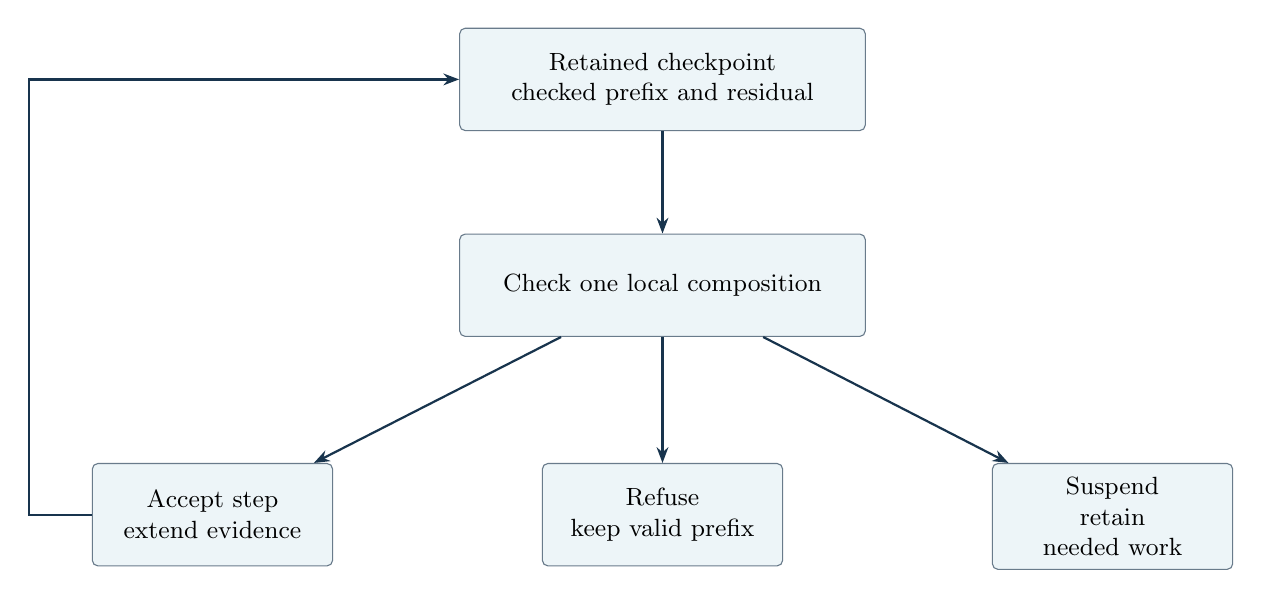
\begin{tikzpicture}
  \node[wide] (saved) {Retained checkpoint\\checked prefix and residual};
  \node[wide,below=13mm of saved] (step) {Check one local composition};
  \node[smallbox,below left=16mm and 16mm of step] (accept) {Accept step\\extend evidence};
  \node[smallbox,below=16mm of step] (refuse) {Refuse\\keep valid prefix};
  \node[smallbox,below right=16mm and 16mm of step] (wait) {Suspend\\retain needed work};
  \draw[arr] (saved) -- (step);
  \draw[arr] (step) -- (accept);
  \draw[arr] (step) -- (refuse);
  \draw[arr] (step) -- (wait);
  \draw[arr] (accept.west) -- ++(-8mm,0) |- (saved.west);
\end{tikzpicture}
\end{center}
\diagramcaption{Missing evidence, exhausted checking budget and an unanswered
external request are different suspension reasons. Refusing the supplied
certificate establishes neither falsity nor unreachability of its claim.}

The retained law is
\[
 \mathsf{advance}(m+n,K)
   =\mathsf{advance}(n,\mathsf{advance}(m,K)).
\]
It compares complete checkpoints. MM0 assertion execution and the HOL Light
source receiver already instantiate \name{ResumableTrajectory}. For MM0,
the command tail and unification continuation remain live; final assertion
validation is a separate observer. For HOL Light, \name{EventWork} retains
the accepted theory/proof state, remaining JSON events and refusal status.
A refused event stays at the residual's head. Accepted receipt prefixes grow
without replay, and two separately identified reflexivity events with the same
conclusion remain two occurrences. The budget counts source events, whose
local costs need not coincide.

The authored recipe DAG and equation-application DAG now have retained
workers over their original nodes and checkers. Each checks one submitted row
per transition, retaining the last accepted table and the entire refused
suffix. Their completed verdicts are exactly the existing certificate
verdicts, and their actual runs finish within the number of rows plus one
finishing transition. The rho tree worker similarly inspects one original
inference occurrence per transition, with exact recursive-checker agreement
and a bound of the tree's node count plus one. Endpoint formation remains an
additional rho request-boundary check. These bounds count calls of the local
worker; they do not price every internal substitution or equality operation.
For authored GSLTs, existence of an actual terminated checker run with an
accepted root is equivalent to inhabiting the existing reaching native type
for an equation-respecting target predicate. The native-type readout therefore
comes from the original finite rewriting semantics, rather than a command
layer with an unspecified local step.

All these workers are objects of the existing machine category at their own
observation interfaces. The MM0 instance keeps its command and unification
microsteps, the HOL Light instance keeps its registered source-event receiver,
and the Lean4Lean head-profile instance keeps its actual head strategy.
Choosing a common observation interface and proving a bounded stage between
two objects are additional obligations. Object construction alone supplies
no translation of one native logic into another.

Retention is governed by future use, not by a requirement to keep every detail
forever. For ordinary value readouts $d$ in a declared consumer family $\mathcal D$,
replacing a detailed record by $q(x)$ is licensed when
\[
       \forall d\in\mathcal D\;\exists\bar d.\qquad d=\bar d\circ q.
\]
Dependent evidence additionally needs coherent family and section descent.
An outstanding obligation must be discharged or transferred under its own
authority contract. Once a recipient owns the needed evidence and every
remaining local consumer factors through the retained summary, the sender
may release detail that no longer serves those obligations. A newly admitted
consumer cannot recover erased distinctions merely by requesting them.

\subsection{A category of machines and realization stages}

For fixed event, verdict and request types $(E,V,Q)$, the existing
\name{ObservedMachine} bundles an actual state carrier $S$ and productive
stepper $M:S\to\mathsf{Option}(\mathsf{Transition}(S,E,V,Q))$.
Its morphisms are the existing \name{Stage} contracts: a relation between
source and target states, a forward cost-bounded simulation and completion
reflection. Identity uses the equality relation at bound one. For stages
$(R,c)$ and $(S,d)$, composition has
\[
 (S\circ R)(x,z)\ \Longleftrightarrow\
       \exists y.\;R(x,y)\wedge S(y,z),
 \qquad \mathsf{cost}=dc.
\]
\name{Stage.refl_comp}, \name{Stage.comp_refl} and
\name{Stage.comp_assoc} supply the category laws. The
\name{ObservedMachine.relabelFunctor} maps a common observation interface
to another while retaining the underlying state carriers. Noninjective label
maps can forget distinctions; each dependent consumer needs its own descent
law before using that coarser view.

\begin{center}
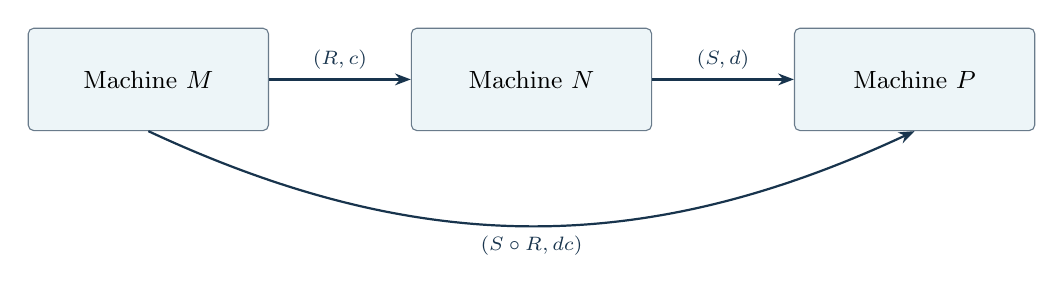
\begin{tikzpicture}
  \node[smallbox] (m) {Machine $M$};
  \node[smallbox,right=18mm of m] (n) {Machine $N$};
  \node[smallbox,right=18mm of n] (p) {Machine $P$};
  \draw[arr] (m) -- node[hint,above]{$(R,c)$} (n);
  \draw[arr] (n) -- node[hint,above]{$(S,d)$} (p);
  \draw[arr] (m.south) to[bend right=25]
    node[hint,below]{$(S\circ R,dc)$} (p.south);
\end{tikzpicture}
\end{center}
\diagramcaption{Composition retains the declared relational contract and
resource bound. It neither selects a compiler implementation nor identifies
all intermediate execution witnesses.}

The controls make the distinction concrete: two stages with bound three
require composite bound nine; the proposed sum six fails. A checker/interpreter
round trip preserves its final observation but differs from the identity
stage because its retained cost bound is three. The bound is a proved account
for the chosen machine transitions, not a measurement of native time.
The present \name{Stage} contract reflects completion; preserving stuckness
versus silent divergence requires further endpoint laws. An existing negative
control relates a stuck source to a spinning target under the weaker contract.
The extra \name{MatchesStuck} obligation excludes that case.

There is also a general finite-trace relational envelope. Fix observable
words $w$, with internal steps erased by a declared observer. For branching
machines, take relations $R$ satisfying
\[
 R(s,u)\ \wedge\ s\overset{w}{\Longrightarrow}_M t
 \quad\Longrightarrow\quad
 \exists v.\;u\overset{w}{\Longrightarrow}_N v\ \wedge\ R(t,v).
\]
Equality is an identity relation. Relational composition preserves this law:
choose the intermediate related state, match the source path in the middle
machine, then match that middle path in the final machine. Relational unit
and associativity laws therefore give a category at this extensional contract
level. This mathematical schema states a finite may-preservation profile;
backward, divergence, probability and resource obligations enrich it separately.
The concrete kernel-checked category above currently uses deterministic
steppers, whose schedules may realize branching source calculi only through
their own adequacy theorem.

Vacuous relations are not executable realizations. Loading must relate every
admitted source entry to an actual target entry; representation, request/reply
and authority laws complete the applicable contract. Furthermore, forgetting
the middle state can erase information required by a dependent result.
\name{DependentComposition.Path} retains that state as data; its descent
theorems identify when transport is independent of the chosen middle witness.
Thus a category of endpoint contracts and a richer account of executions can
coexist, with information release justified at the selected boundary.

For the MeTTa realizations, the realization obligations are stated at semantic
operations: complete occurrence selection, solution-preserving binding reads
and merges, retained call/return control, and world/dependency/publication
updates. An implementation may realize one such operation by a size-dependent
finite block. Storage layouts and individual C helpers lie downstream of this
boundary. Their existing formal proofs are worked representation instances;
they do not enlarge the logical machine or require a new source rule for
each helper. Formal local simulation laws, source/ABI premises and tests of a
compiled engine are distinct evidence. A tested binary link cannot substitute
for a required unproved formal component law.

The common realization boundary is now explicit in
\name{ProductiveCoreAdapters.ComponentRealization}.  A
\name{ComponentProjection} exposes store, control, selection, world and
publication.  A \name{FiveComponentRel} gives each projection its own
relation and adds one joint coherence law.  Its state relation
\name{Holds} is the conjunction of those six obligations; no component can be
replaced by \name{Unit} or an always-true relation without changing the
contract.  A \name{ProductiveLocalBlock} requires every logical inspection to
be implemented by a nonempty finite target derivation with the declared public
events and endpoint relation.

\name{ModularMachineAdequacy} records M1--M7: related loading, complete
selection observation, certified store reading, the productive control block,
world observation, retained-control observation, and publication/future-use
observation.  M8 is deliberately absent as a field.
\name{toDerivationSimulation} derives it from the local block, after which
\name{loaded_prefix}, \name{loaded_completed} and
\name{loaded_retained_run} use the common span-transport theorems.  The retained
theorem starts the implementation suffix at the implementation endpoint of its
prefix and returns agreement of all five semantic observations there.  Thus a
complete evaluator run cannot be smuggled into a component premise.

The HE restore-profile instance uses the same stateful contextual
\name{Protocol.Rule} on both sides and a nonidentity
\name{RestoreRepresentation} load between solution-equivalent binding
presentations.  Joint model reads, saved continuations, current selection space,
world, publication bag and future \name{Frame.read} observations agree;
\name{restore_productive_block} proves the local protocol step.  This is a
representation-independence result at a restore cut, not a refinement from the
AM to a different runtime machine.  The PeTTa instance does relate different
step relations: an ordinary pre-return state to its protected
\name{attachState}.  Binding equations, physical
context/origin occurrences, world and collected answers remain exact, while
the active goals receive the shifted saved suffix and parent controls do not
move.  \name{preReturn_derivation_attach} earns the productive target block,
and the existing scoped source/runner theorem executes it.

\subsection{Fibres, crossings and a machine of machines}

The functional GSLT construction is already literal category theory.
\name{OperationalTranslation} preserves equations and source steps;
\name{CoveredTranslation} additionally covers target steps at image states.
The functor \name{executionIndex} sends each operational theory $L$ to its
category of finite execution paths. Its Grothendieck construction has objects
$(L,s)$ and arrows
\[
 (L,s)\longrightarrow(K,t)
 \quad=\quad
 \bigl(f:L\to K,\;p:F(f)(s)\longrightarrow t\bigr).
\]
For $f:L\to K$, $g:K\to H$ and compatible paths $p,q$, the composite is
$(g\circ f,F(g)(p);q)$. Identity and associativity follow from the base and
fibre laws and the functor laws. This is a constructed total category for
functional operational transport. Its underlying proposition-valued steps do
not distinguish two rule occurrences with identical endpoints; receipts or
labelled edges retain such distinctions when required.

\begin{center}
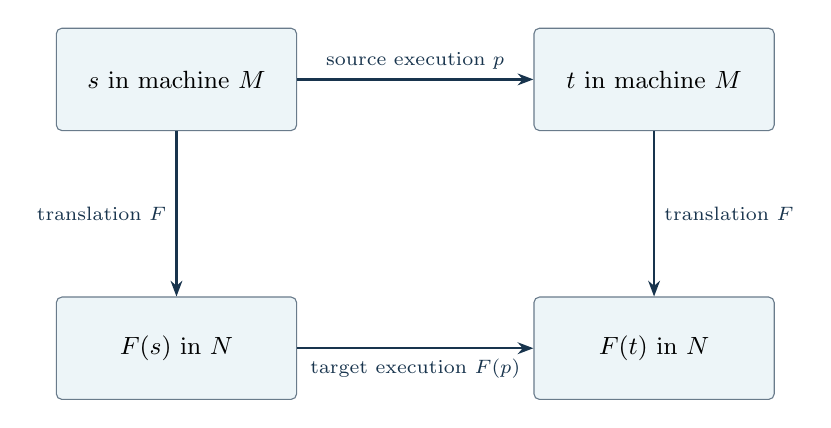
\begin{tikzpicture}
  \node[smallbox] (s) {$s$ in machine $M$};
  \node[smallbox,right=30mm of s] (t) {$t$ in machine $M$};
  \node[smallbox,below=21mm of s] (fs) {$F(s)$ in $N$};
  \node[smallbox,right=30mm of fs] (ft) {$F(t)$ in $N$};
  \draw[arr] (s) -- node[hint,above]{source execution $p$} (t);
  \draw[arr] (s) -- node[hint,left]{translation $F$} (fs);
  \draw[arr] (t) -- node[hint,right]{translation $F$} (ft);
  \draw[arr] (fs) -- node[hint,below]{target execution $F(p)$} (ft);
\end{tikzpicture}
\end{center}
\diagramcaption{A functional path map supplies a commuting square. Relational
block simulations instead retain related endpoints and their actual matching
paths; their coherence is an additional construction.}

The executable \name{GSLTILNativeKernel} separates stepping inside a fibre
from crossing an explicit route. The installed \name{GSLTILAuthoredFibre}
uses the actual authored rewrite checker and its source-coverage theorem.
It currently installs no translation routes. Its \code{at}/\code{via}
dispatcher can host locally justified routes, but does not manufacture their
interpretations, resource transport or conservativity.

A broader web can retain relational simulations and comparison cells instead
of forcing all crossings into state functions. Horizontal paths then concern
executions within a regional machine; vertical comparisons relate configurations
of different machines; a cell supplies the matched execution evidence. These
cells need their own composition and coherence laws. Substitution, logical
interpretation, world update and authority transport retain different
preservation contracts even when they occur in one diagram. This is the
remaining generalization, not an implication of the Grothendieck name.

\subsection{Regional kernels, semantic faces and open-ended reflection}

The checking machine has an operational run; its accepted evidence inhabits
an intensional derivation judgment; model interpretation supplies an
extensional face. These comparisons form the computational trinity around the
checker. Logical soundness goes from derivations to validity in the selected
models. Logical completeness, where established for the particular fragment,
goes in the other direction. Coverage of certificate representations is
instead a comparison with derivations. These three claims have different
hypotheses and do not identify the faces.

MM0 makes the distinction between its readable specification and binary proof
program explicit~\cite{MM0}. Its verifier computes with stacks, hypotheses,
terms and binder data, and declaration agreement binds that computation to
the intended specification and preceding environment. HOL Light supplies
kernel-authorized inference through the LCF interface~\cite{HOLLight}; its
theorem cache and receipt graph have a separate retained execution account.
Megalodon checks typed proof objects with normalization and delta expansion
under its selected environment. OpenTheory articles give a textual proof
stack machine~\cite{OpenTheoryArticle}; CakeML includes a verified article
checker and Candle's HOL Light implementation~\cite{CakeMLProofMachines}.
These are regional realizations, with distinct logical commitments and
checking disciplines.

Lambdapi and HOL Light exercise different binder obligations. Lambdapi's
restricted higher-order rewrite patterns test scoped matching under
binders~\cite{LambdapiRules}. HOL Light's primitive replay tests term/type
instantiation and theorem construction. Real HE and PeTTa evaluation kernels
must likewise use their own independent judgments: a certified rewrite at one
atom's root does not establish the dialect's nested evaluation, quoted/raw
arguments, complete result multiplicity or retained effects.

Structural compilation of an admitted profile and checking a finite execution
are complementary hosting routes. Partial recursive checkers admit finite
bounded-evaluation witnesses~\cite{MathlibPartrecCode}; actual hosting still
requires the source encoding, target certificate construction and checker
adequacy. A p-simulation further requires a polynomial-time proof translator
under declared encodings, hence polynomial output size. A short operation
name does not make a large substitution or conversion cheap. Shared-node
size, expanded uses and executed work require separate accounts.

Small primitive inventories, weak logical assumptions and cheap checking are
different objectives. The existing inference-basis theory supplies
inclusion-minimal generating subsets for a finite inventory, including
incomparable minima with no least generating basis. It supplies neither an
efficient minimizer nor a universal least kernel. The common interface is
licensed composition; individual presentations choose their generating rules
and prove their interpretation.

An interactive prover additionally retains open goals, scoped metavariables,
substitutions and delayed constraints. Its search may diverge or remain
incomplete even when each closed certificate is finitely checkable. Reflection
makes these presentations and checking processes available as data. Goertzel's
reflective metagraph account motivates this internal availability of rules and
their transformations~\cite{ReflectiveMetagraph}. Weinbaum's open-ended
intelligence motivates admitting new vocabularies and observers rather than
requiring a final fixed inventory~\cite{WeinbaumThesis}. The architectural
proposal is to combine that openness with explicit crossings: changing a
theory exposes new commitments, replacing a machine preserves the declared
observations, and neither silently changes what an earlier certificate proved.

\sources{\name{Mettapedia/Logic/DerivationGraph.lean},
\name{Mettapedia/GSLT/LanguageDef/CertificateGSLTClassifyingCategory.lean},
\name{Mettapedia/OSLF/MeTTaIL/GeneralRewriteRecipe.lean},
\name{Mettapedia/OSLF/MeTTaIL/GeneralRewriteRecipeExpansion.lean},
\name{Mettapedia/OSLF/MeTTaIL/GeneralRewriteRecipeComposition.lean},
\name{Mettapedia/OSLF/MeTTaIL/GeneralRewriteRecipeContext.lean},
\name{Mettapedia/OSLF/MeTTaIL/GeneralRewriteRecipeDAG.lean},
\name{Mettapedia/OSLF/MeTTaIL/GeneralRewriteRecipeExecution.lean},
\name{Mettapedia/OSLF/MeTTaIL/GeneralRewriteRecipeParallel.lean},
\name{Mettapedia/GSLT/Distinction/SimulationComposition.lean},
\name{Mettapedia/GSLT/Distinction/SimulationCompositionControls.lean},
\name{Mettapedia/GSLT/Distinction/DependentComposition.lean},
\name{Mettapedia/GSLT/Core/OperationalPathFibration.lean},
\name{Mettapedia/GSLT/LanguageDef/GSLTILAuthoredFibre.lean},
\name{Mettapedia/Languages/MM0/Formats/MMB/MachineCost.lean},
\name{Mettapedia/Languages/MM0/MeTTa/Formats/MMB/ExecutedSoundness.lean},
\name{Mettapedia/Languages/HOLLight/IncrementalExecution.lean},
\name{Mettapedia/Languages/HOLLight/KernelAtlas.lean},
\name{Mettapedia/Languages/MeTTa/EquationKernel/Execution.lean},
\name{Mettapedia/Languages/ProcessCalculi/RhoCalculus/NativeExecution.lean},
\name{Mettapedia/Languages/Lean/HintedHeadConversion.lean},
\name{Mettapedia/Languages/Lean/Lean4LessCheckerBoundary.lean},
\name{Mettapedia/Logic/EqualityRecipe.lean},
\name{Mettapedia/Computability/FuelledConversionEvidence.lean},
\name{Mettapedia/Machines/ExecutionHints.lean},
\name{Mettapedia/GSLT/LanguageDef/KernelCheckingClasses.lean},
\name{Mettapedia/GSLT/Logic/PropositionalLRAT.lean},
\name{Mettapedia/Logic/PropositionalExtension.lean},
\name{Mettapedia/Logic/IntuitionisticDecision.lean},
\name{Mettapedia/Logic/PropositionalHilbertChecking.lean},
\name{Mettapedia/Logic/ProofSharingBounds.lean},
\name{Mettapedia/Coalgebra/CoherentPrefixTower.lean},
\name{Mettapedia/Logic/InferenceBasis.lean}.}
\scope{Local authored checking, its composition operations, functional path
transport, costed stage composition, checked reconstruction and the retained
native checker instances are constructed at their stated contracts. Authored packet coverage
uses the existing admission compiler and an empty dynamic provider; textual
module parsing is a separate front end. The finite-trace
relational envelope is a mathematical schema. A complete heterogeneous
execution/certificate web, its route authentication, general relational
coherence and native physical resource bounds remain further constructions.}


\newpage
\section{Execution contracts: determinism is one dimension}
\label{sec:contracts}

A deterministic implementation can enumerate many answers, compute an entire
distribution, or simulate concurrent processes under a selected schedule.
A sampler can return exactly one answer while representing a nontrivial
probability law. These properties therefore cannot be represented by one
exclusive choice between deterministic, nondeterministic and probabilistic.

\begin{tabularx}{\linewidth}{@{}p{34mm}XX@{}}
\toprule
Dimension & Contract question & Distinguishing example \\
\midrule
Transition & At most one next state? & An ordered search driver steps
deterministically through many alternatives. \\
Cardinality & How many successful occurrences in a completed run? & Two equal
answers count twice. \\
Completion & Is any work still pending? & One answer followed by a suspended
branch is not a closed singleton. \\
Probability & What measure describes outcomes? & A fair and a biased coin
have the same finite support. \\
Concurrency & Which enabled actions may be scheduled? & Two independent
actions can commute without one global deterministic schedule. \\
Commitment & Which alternatives or effects may be discarded? & \code{once}
selects a success; it does not prove there was only one. \\
\bottomrule
\end{tabularx}

\subsection*{Cardinality belongs to a calling mode and its world}
The existing answer grades bound the number of occurrences in a completed
answer collection: zero, exactly one, zero-or-one, one-or-more, or unrestricted.
Relational choice adds occurrence counts; an exclusive conditional combines
bounds by an interval hull. Sequential binding applies a bound separately
to each reachable input occurrence with its bindings. Types, instantiation,
termination, faults and effects remain additional obligations. A declaration
of \code{det} expresses a contract; an optimization needs evidence for the
actual calling mode and relevant provider revision.

The current weighted cardinality consumer accepts a complete cut only when
it is empty or contains one returned occurrence. It preserves that occurrence's
coefficient, including zero. A cut with a pending state is refused even if
its current returned prefix has length one. The accepted result is stable
under further resumption. This is a representation theorem about an already
computed cut, not a procedure for deciding termination or safely pruning
an unfinished search. Probing for another answer can perform effects,
force otherwise unused work, or diverge.

\subsection*{What a deterministic region can improve}
The independently defined queued and direct executors already agree on
ready operands, functional primitives, worlds, ordered effects, failures and
instruction-boundary residuals. Their primitive invocation counts agree;
their modeled dispatch counts differ. This licenses eliminating that queue
within the admitted region. It establishes no native speedup and does not
yet cover arbitrary expressions, binding merges or concurrent mutation.

\sources{\name{Mettapedia/Machines/AnswerCardinality.lean},
\name{Mettapedia/Machines/DeterministicRegion.lean},
\name{Mettapedia/Machines/OccurrenceMachine.lean},
\name{Mettapedia/GSLT/Dynamics/WeightedBranchingCardinality.lean}.}

\newpage
\subsection{Probabilities, coefficients and schedules}

A coefficient is not automatically a probability. The weighted resumption
interfaces work with algebraic coefficients and preserve pending contributions
and occurrence identity. A probabilistic interpretation additionally needs
nonnegative mass and a specified normalization or subnormalization law.
An importance weight, a scheduling priority, a cost and an ownership permission
are different quantities even when they use similar algebraic notation.

\begin{center}
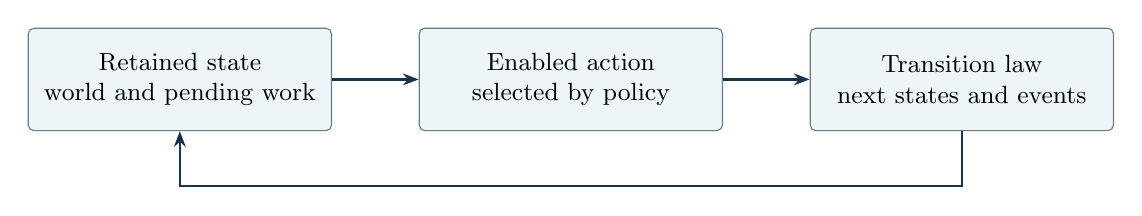
\begin{tikzpicture}
  \node[box] (state) {Retained state\\world and pending work};
  \node[box,right=11mm of state] (action) {Enabled action\\selected by policy};
  \node[box,right=11mm of action] (law) {Transition law\\next states and events};
  \draw[arr] (state) -- (action);
  \draw[arr] (action) -- (law);
  \draw[arr] (law.south) -- ++(0,-7mm) -| (state.south);
\end{tikzpicture}
\end{center}
\diagramcaption{A scheduler selects an enabled action; a probabilistic kernel
specifies its stochastic transition. Relational alternatives need not carry a
canonical probability law. A point mass recovers deterministic transition.}

Combining nondeterministic choice with probability is a semantic choice:
the available scheduler information and the order of the two effects matter.
One cannot assume that an arbitrary combination of the familiar monads has
the desired distributive laws~\cite{ProbNondet}. A machine contract should
state the admissible policies and what the observer compares: possibilities,
ordered occurrences, trace distributions, or another declared quantity.

The existing finite probabilistic systems use subdistributions and account
for missing mass as declared refusal. Their probabilistic bisimulation retains
more information than the support relation. However, the system record does
not itself prove that its kernel follows the underlying GSLT rewrite relation;
that is an operational bridge still to construct. Erasing probabilities to
possibility support cannot justify a probability-preserving implementation.
For a continuous distribution, a singleton can have probability zero without
being an impossible value; positive point mass is not a general support test.

\subsection*{Sampling, scoring and resumption}
A retained draw needs its dynamic occurrence identity and original world.
Resuming a committed draw must reuse its result. Calling a resampled suspension
creates a new occurrence; merely sharing written syntax does not establish
stochastic independence. Independence requires a law for the actual joint
execution, often conditional on captured latent variables.

Scoring generally produces an unnormalized measure. Forming a posterior
requires an evidence mass $Z$ with $0<Z<\infty$; zero or infinite evidence
needs explicit treatment. Retention must preserve committed factors and avoid
applying them again. Existing coefficient plumbing is useful here, but it
does not supply this entire probability-and-authority contract.

\scope{No production port is licensed solely by cardinality or coefficient
laws. The complete world, bindings, effect history, faults, ownership and
residual demand must travel through the same constructed correspondence.}

\sources{\name{Mettapedia/GSLT/Dynamics/WeightedResumption.lean},
\name{Mettapedia/GSLT/Dynamics/WeightedBranchingResumption.lean},
\name{Mettapedia/GSLT/Distinction/Probabilistic/System.lean},
\name{Mettapedia/GSLT/Distinction/Probabilistic/Semiring.lean},
\name{Mettapedia/ProbabilityTheory/IndependentFiniteSampling.lean}.}

\newpage
\section{Focus, zippers and typed graph holes}
\label{sec:holes}

For regular tree syntax, the derivative of a datatype describes its one-hole
contexts~\cite{Derivative}. A zipper retains a focused subtree and the
context needed to rebuild its surroundings~\cite{Zipper}. Indexed
polynomials extend this organization with context and sort information;
dissections distinguish already processed positions from remaining positions.
These are representation and navigation tools. A legal position is not by
itself permission to evaluate, force, sample or commit an effect.

\begin{center}
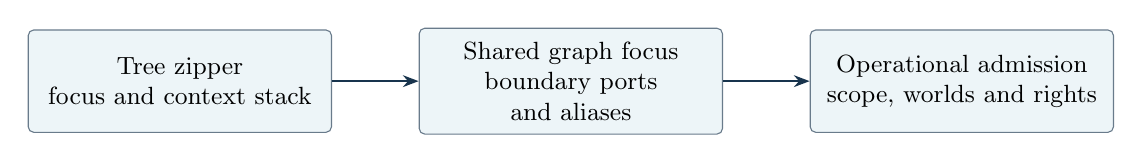
\begin{tikzpicture}
  \node[box] (tree) {Tree zipper\\focus and context stack};
  \node[box,right=11mm of tree] (graph) {Shared graph focus\\boundary ports and aliases};
  \node[box,right=11mm of graph] (rights) {Operational admission\\scope, worlds and rights};
  \draw[arr] (tree) -- (graph);
  \draw[arr] (graph) -- (rights);
\end{tikzpicture}
\end{center}

The existing PathMap zipper interface transports query membership under
iteration and store-agreement hypotheses. Concrete flat and trie instances
prove particular traversal and rebuilding laws. This is useful ZAM structure;
it is not a proof of the full native Rust machine, ordered query multiplicity,
or its world and demand semantics. A membership theorem alone cannot establish
that two equal rows produce two answer occurrences.

\subsection*{A shared hole needs an interface, not just a path}
Replacing a shared subgraph affects every alias to it. A graph hole therefore
needs the incoming and outgoing ports crossing its boundary, their scoped
types, identity and sharing requirements, and the resources or obligations
that move with them. A single tree path loses those other connections.
Cycles require the corresponding consistency and update rules. Bag or set
quotients also need occurrence identities when their physical ordering is
not canonical.

Goertzel's reflective metagraph account makes programs and rewrite rules
graph data~\cite{ReflectiveMetagraph}. Graph rewriting's preserved interface
and gluing conditions are useful guidance: a replacement must account for
the links it preserves and those it removes. This motivates a runtime contract;
it does not already provide a typed effectful graph-hole machine.

\subsection*{Different holes have different filling rules}
An unknown source fragment, a paused computation, a stochastic latent variable,
an external response and an unfulfilled proof obligation are not interchangeable.
The existing pure higher-order hole evaluator retains environments and
indeterminate operations. Its filling/resumption equivalence has a termination
condition. Its controls show that divergent call-by-value fillers and effectful
reordering can break an unrestricted equivalence. The tree multi-hole monad
also deliberately permits capture; it is not a ready-made hygienic shared-graph
interface. Filling must establish the applicable scope and execution contract.

\sources{\name{Mettapedia/GSLT/Poly/BindingSignature.lean},
\name{Mettapedia/GSLT/Poly/SortedTraversal.lean},
\name{Mettapedia/OSLF/PathMap/ZipperExecution.lean},
\name{Mettapedia/OSLF/PathMap/Trie/HuetZipper.lean},
\name{Mettapedia/OSLF/Programs/HoleEvaluation.lean},
\name{Mettapedia/OSLF/MeTTaIL/MultiHoleContext.lean},
\name{Mettapedia/GraphTheory/Representation/Metagraph.lean}.}

\newpage
\subsection{A core MAM for heterogeneous retained computations}

The strongest candidate here separates execution, dependency accounting and
reflection. They refer to the same occurrence identities, but they need not
use one physical representation. A machine can execute a compact packed
region while exposing a metagraph view on demand. Reflection need not allocate
a public syntax object for every primitive instruction.

\begin{center}
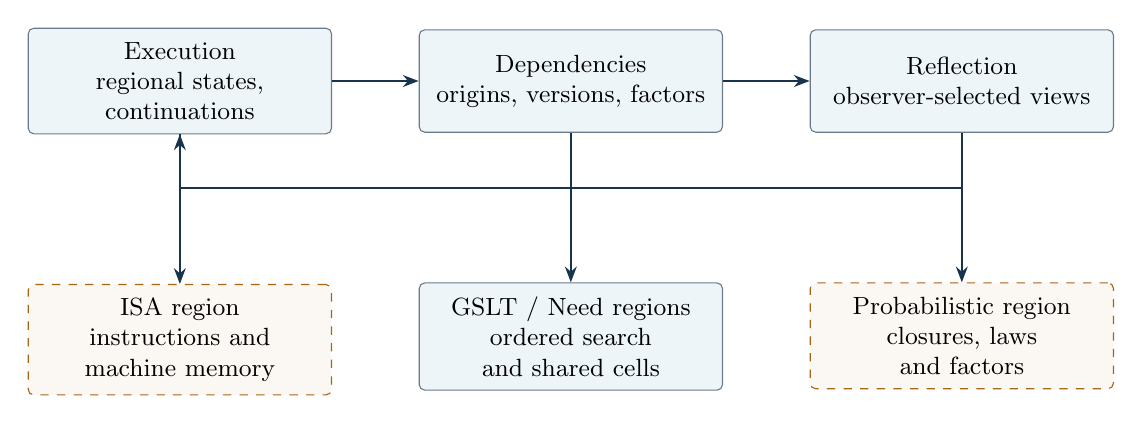
\begin{tikzpicture}
  \node[box] (execution) {Execution\\regional states, continuations};
  \node[box,right=11mm of execution] (dependency) {Dependencies\\origins, versions, factors};
  \node[box,right=11mm of dependency] (reflection) {Reflection\\observer-selected views};
  \draw[arr] (execution) -- (dependency);
  \draw[arr] (dependency) -- (reflection);
  \draw[arr] (reflection.south) -- ++(0,-7mm) -| (execution.south);
  \node[future,below=19mm of execution] (isa) {ISA region\\instructions and machine memory};
  \node[box,below=19mm of dependency] (gslt) {GSLT / Need regions\\ordered search and shared cells};
  \node[future,below=19mm of reflection] (ppl) {Probabilistic region\\closures, laws and factors};
  \draw[arr] (execution) -- (isa);
  \draw[arr] (dependency) -- (gslt);
  \draw[arr] (reflection) -- (ppl);
\end{tikzpicture}
\end{center}
\diagramcaption{Dashed regions mark unconstructed general interfaces. All regional
calls use the crossing contract; the connecting lines do not assert an ISA or
higher-order probability correspondence already exists.}

The proposed retained state includes local computations, typed open boundaries,
shared producer/use identities, ordered alternatives, world dependencies,
committed draws and factors, consumed rights, and selected observations.
Its transitions admit and focus a region, advance it, deliver a request or
reply, fill an authorized hole, validate dependencies, pause, or dispose of
cancelled obligations. Sampling and scoring come from an admitted regional
semantics. Neither graph shape nor a type annotation silently authorizes them.
Logical guests retain their own judgment systems; a common port protocol
does not make their propositions interchangeable.

Qualification would lift local correspondences through admitted graph
contexts, fillings and crossings. At publication, suspension and return,
the chosen trace observations and related residuals must survive together.
Probabilistic regions compare the resulting laws under declared scheduling
policies, or a stated coupling bound; equal possible values are insufficient.
These compatibility laws must be proved for the actual assembly. Listing
types and authority metadata does not establish them.

An ISA region would load code with an instruction-validity contract and retain
registers, memory, faults and external-service state. Its source translation
must state ABI and memory assumptions. The existing register-code machine
supplies a narrower lowering and execution connection; a proposed
\code{lts:isa} interface is not established by that result. Cesta macro
elaboration belongs to a staging phase, before the resulting C/native region.

A GSLT interpreter is a general rule-execution machine. Calling it UTM-tier
requires an encoding of universal computation and a correspondence theorem.
Even such a theorem would not preserve fairness, ordered occurrences, costs,
probability laws or ownership automatically. Those are regional contracts,
not consequences of computational universality.

\scope{This architecture is a research target assembled from existing owners.
It is not an implemented universal MAM or a claim that one representation is
optimal for every region. Its first consumer remains the actual MeTTa
source/native and owned-interaction connection.}

\sources{\name{Mettapedia/Machines/RegisterCode.lean},
\name{Mettapedia/Languages/TuringMachine/MathlibBridge.lean},
\name{Mettapedia/GSLT/Dynamics/ObservationSchedulerSufficiency.lean},
\name{Mettapedia/GSLT/Dynamics/ScheduleObservationFactorization.lean}.}

\newpage
\section{Higher-order probabilistic holes}

Consider a hole with type
\[
 \Box_{\mathrm{make}}:\mathrm{Unit}\longrightarrow
 \mathcal P(\mathrm{Unit}\longrightarrow\mathcal P\mathrm{Bool}),
\]
where $\mathcal P$ denotes a probability computation. A consumer obtains
$f$ from \code{make ()}, calls $f$ twice, and returns the pair $(a,b)$.
There are two well-typed fillings:

\begin{tabularx}{\linewidth}{@{}>{\raggedright\arraybackslash}X>{\raggedright\arraybackslash}X@{}}
\toprule
Shared draw & Fresh draw per call \\
\midrule
\code{cached () =} & \code{fresh () =} \\
\quad draw $z\sim\operatorname{Bernoulli}(1/2)$ &
\quad return a closure which, on every call, draws a fresh
$z\sim\operatorname{Bernoulli}(1/2)$ and returns $z$. \\
\quad return $(\lambda().\ \text{return }z)$ & \\
\bottomrule
\end{tabularx}

Both give a fair marginal for either individual call. Their joint laws differ:

\begin{center}
\begin{tabular}{@{}lrrrr@{}}
\toprule
Filling & $(0,0)$ & $(0,1)$ & $(1,0)$ & $(1,1)$ \\
\midrule
Shared draw & $1/2$ & $0$ & $0$ & $1/2$ \\
Fresh draws & $1/4$ & $1/4$ & $1/4$ & $1/4$ \\
\bottomrule
\end{tabular}
\end{center}
Thus $\Pr(a=b)$ is respectively $1$ and $1/2$. Matching the hole's type or
one call's marginal cannot license replacing one filling by the other.
One shared draw has one producer with two use edges; two independent draws
have two dynamic sampling occurrences, even if their source syntax is equal.

\begin{center}
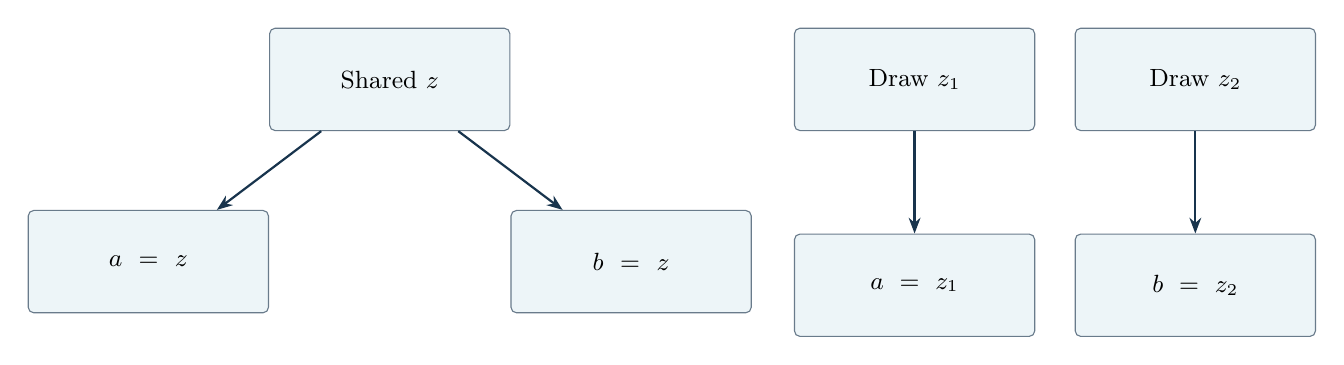
\begin{tikzpicture}
  \node[smallbox] (z) {Shared $z$};
  \node[smallbox,below left=10mm and 0mm of z] (a) {$a=z$};
  \node[smallbox,below right=10mm and 0mm of z] (b) {$b=z$};
  \draw[arr] (z) -- (a); \draw[arr] (z) -- (b);
  \node[smallbox,right=36mm of z] (u) {Draw $z_1$};
  \node[smallbox,right=5mm of u] (v) {Draw $z_2$};
  \node[smallbox,below=13mm of u] (c) {$a=z_1$};
  \node[smallbox,below=13mm of v] (d) {$b=z_2$};
  \draw[arr] (u) -- (c); \draw[arr] (v) -- (d);
\end{tikzpicture}
\end{center}

\subsection*{Two semantic routes remain open}
An operational route places measures over encoded closures and retained
machine states, with application specified by the evaluator. A denotational
route supports function spaces directly. Ordinary measurable spaces are
insufficient for the desired general higher-order structure; quasi-Borel
spaces provide a compositional alternative~\cite{QBS}, with domain-theoretic
extensions for recursion and recursive types~\cite{ProbDomains}.
Neither route should be confused with the existing mixture-of-kernels or
probabilistic-HOL-model modules, which do not implement a general probabilistic
lambda calculus. The small example above is a mathematical discriminator,
not a newly proved machine instance.

\sources{\name{Mettapedia/ProbabilityTheory/HigherOrderProbability/Basic.lean},
\name{Mettapedia/ProbabilityTheory/HigherOrderProbability/GiryMonad.lean},
\name{Mettapedia/ProbabilityTheory/IndependentFiniteSampling.lean}.}

\newpage
\subsection{Zooming requires a law for future computation}
\label{sec:zoom}

Let $v:S\to C$ forget details of a fine state. Equal coarse readouts now
are insufficient: different hidden states can react differently to the next
command. An exact coarse machine needs a law relating its future transitions
to those of the fine machine, for the declared action and observer family.

\begin{center}
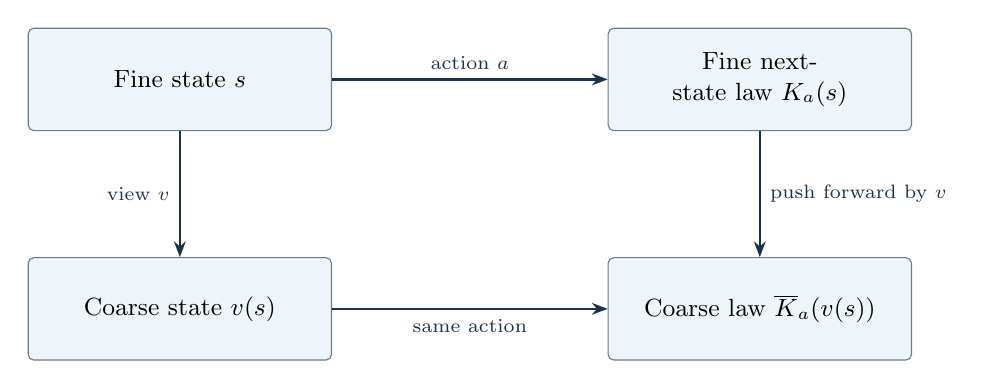
\begin{tikzpicture}
  \node[box] (s) {Fine state $s$};
  \node[box,right=35mm of s] (next) {Fine next-state law $K_a(s)$};
  \node[box,below=16mm of s] (coarse) {Coarse state $v(s)$};
  \node[box,below=16mm of next] (coarsenext) {Coarse law $\overline K_a(v(s))$};
  \draw[arr] (s) -- node[hint,above]{action $a$} (next);
  \draw[arr] (s) -- node[hint,left]{view $v$} (coarse);
  \draw[arr] (next) -- node[hint,right]{push forward by $v$} (coarsenext);
  \draw[arr] (coarse) -- node[hint,below]{same action} (coarsenext);
\end{tikzpicture}
\end{center}

For finite probabilistic states, existing strong lumpability says that states
in one view fibre have the same aggregated next-state law for every admitted
action. It constructs a representative-independent coarse kernel and proves
\[
 v_*\bigl(\mu\mathbin{\mathrm{bind}}K_a\bigr)
   =(v_*\mu)\mathbin{\mathrm{bind}}\overline K_a.
\]
Here $v_*$ is pushforward. Without this condition, retain additional state or
history, restrict actions/observers, or accept a weaker approximate contract.
A policy depending on hidden details also needs its own factorization law.

Existing probabilistic-square results offer a finite controlled-chain route
to approximation: local couplings bound expected discrepancy, and Lipschitz
and discount hypotheses control its accumulated observational effect.
They are not exact quotients or reversible maps. Numerical closeness also
depends on the observer: a finite floating-point distribution and a continuous
law can be maximally different in total variation despite close numerical
samples. A metric suited to the permitted queries may be more appropriate.

Zooming in can expose retained fine state or reconstruct an authorized view.
It cannot recover arbitrary forgotten choices from a non-injective quotient.
For the shared-draw example, the first call's marginal hides the captured
draw and whether subsequent calls reuse it; reconstructing by resampling
can break those correlations. Similarly,
replaying a native trace must not repeat committed effects. Observation,
demand and retention therefore remain separate in-language controls.

\subsection*{The remaining research question}
The missing joint theory is typed open-metagraph filling with scope, shared
identity, effects, probability and ownership, together with observation maps
that commute with continuation. Useful research would compare existing
models, identify incompatibilities, and work one higher-order shared/fresh
example through both exact finite execution and a continuous denotation.
General recursion, conditioning and scheduling must keep their explicit
conditions; universal complete inference is not a consequence of a universal
machine.

\sources{\name{Mettapedia/ProbabilityTheory/FiniteLumpability.lean},
\name{Mettapedia/Cybernetics/ApproximateAdequacy/ProbabilisticSquares.lean},
\name{Mettapedia/GSLT/Dynamics/ObservationSchedulerSufficiency.lean},
\name{Mettapedia/GSLT/Dynamics/ScheduleObservationFactorization.lean}.}

\newpage
\section{Qualification and closure}

The principal inventory is maintained with the eight accepted obligations:
common operational theory, historical CAM, fixed C, HE/PeTTa correspondence,
shared and distinct dialect behavior, retention/interaction, component
realization, and joined qualification. It indexes existing declarations by
source contract, observer and assumptions. Historical proof and test receipts
remain evidence for their recorded source states; they are not current
qualification after a dependency changes.

\subsection*{What the principal theorems establish}

{\small
\begin{tabularx}{\linewidth}{@{}>{\raggedright\arraybackslash}p{27mm}>{\raggedright\arraybackslash}X@{}}
\toprule
Layer & Constructed connection and boundary \\
\midrule
Common theory &
\name{DerivationSimulation.transport}, \name{trans} and \name{resume}
compose constructed local blocks. \name{CostSimulation.toDerivationSimulation}
requires \name{MatchesStuck}. \name{EventCursor.advance_simulation} and
\name{resume_simulation} reach actual scheduled execution. The HE and PeTTa
instances below construct the required local laws; the generic theorem alone
still makes no compiled-runtime claim. \\
CAM &
Historical compiler/readback, typed strict meaning, graph recursion and Need
have their independent source correspondences. Graph/tree scheduled refinement
and abstraction use nontrivial representation maps. Original coverage and
the named importing consumers are included in the joined qualification. \\
Fixed C &
\name{FixedCore.Scheduled.source_path_iff} preserves permitted choices and
retained supply. Cesta reading, the stated fixed/located fragment and service
calls have separate correspondences. A compiled CeTTa program is not thereby
a program of the fixed core; the named extension ledger remains authoritative.
\\
HE source/AM &
\name{Contextual.source_iff_observed} and
\name{Protocol.public_completion_iff_source} connect independent completed
source judgments, actual contextual paths and joint caller/value answer bags.
The stateful correspondence additionally retains its reached world. The full
contextual grammar, the narrower worker profile and external services retain
their separately stated boundaries. \\
HE worker &
The declared plain-Atom worker has earned typed/cast/failed-selection,
selected-function, tuple, ordinary-call and finite ranked-fallback recursion.
\name{ScopedRankedFallbackStep} closes fallback nesting outside the dependent
mutual families. Held readiness, embedded minimal instructions and the full
contextual grammar stay explicit negative boundaries of this representation;
the full HE machine is the contextual AM above. \\
PeTTa &
\name{Scoped.source_run_iff_derivation} and \name{completed_iff_source}
cover finite scoped source execution; \name{commit_first_answer} reaches an
answer without waiting for younger search to finish. Protected pre-return
attachment now instantiates the component-realization interface; wider native
dialect conformance remains separate tested evidence. \\
Shared fragment &
\name{recursive_machine_bag_iff} and
\name{recursive_machine_storage_permutation} preserve the admitted pure
recursive fragment's multiplicities and protected caller observations. Its
closed profile uses materialized inputs. For the open profile,
\name{OpenRecursive.Evaluation.transport} constructs the HE derivation and
source branch paths from one complete recursive source tree, preserving the
ordered list and bag of joint caller/value observations.
\name{CollectionLinearization.Evaluation.realize_root} composes that theorem
with an earned \name{CollectionScope} DFS drain for the same tree. It preserves
source order, duplicate occurrences, physical origins, live freshening support
and the exact outer pending frontier. Grounded services and wider controls
remain separate profiles. \\
Interaction &
The weighted Need theorem separately preserves its finite dependent-chain
multiplicities. \name{composed_retention_no_replay} is the HE shared-state join:
one \name{JoinedState} path performs the dependency-checked append, consumes the
matching issued row, and caches that exact delivered configuration for later
Need demands without invoking the producer again.  The scoped PeTTa join
combines cut execution, scheduler resumption and shared-graph lifetime.
Disjoint COMM publications commute under their stated read/write independence,
while consumed occurrences and reply handles cannot be replayed. \\
Realization &
\name{ModularMachineAdequacy} discharges M1--M7 through five explicit component
relations and derives M8.  HE restore-presentation invariance and PeTTa
protected-continuation attachment are maintained nonidentity profiles; the HE
profile deliberately uses one rule relation, while PeTTa relates two. Existing
reader, open-slot, C-memory and ABI results remain downstream component
examples; they do not imply correctness of every compiled binary. \\
\bottomrule
\end{tabularx}%
}%
\subsection*{Readout equivalence does not erase operational distinctions}

A binding observation is joint:
\[
  \mathsf{observedTuples}(B,\vec a)
     =\{\sigma(\vec a)\mid\sigma\models B\}.
\]
This preserves repeated-variable correlation, while separate scalar observers
can lose it. A \name{ReadoutCertificate} connects one retained normal table
to the complete constraint theory and supports future operands and independent
constraint extension. Hygiene support is separate: a redundant equality can
change the names that must be protected without changing the solution set.

Changing a constraint record through \name{Frame.represent} retains its exact
annotated environment. Changing that environment to another model-equivalent
representative is a stronger operation. Opposite open-variable representatives
can give the same joint observations but different literal syntax at the next
atom dispatch. The worker's canonical control simulation consequently uses
\name{ScopedActivationRel} and earned entry/materialization admission; the
general finite-model cast result uses joint observational adequacy instead.
Neither theorem may be substituted silently for the other.

Readiness has the same boundary. Equal erased constraints do not determine
whether an expression is active or held. The contextual machine retains that
status under the selected policy, whereas the plain-Atom worker is a stripped
representation with a narrower admission. Its private-sibling freshness law
protects both substitution keys and variables occurring in stored values.
A materialized open result instead earns stable entry from the certified
normal read. General recursive realization must preserve the appropriate
invariant at every reached call and return; it cannot assume all caller
variables remain private or unassigned.

\subsection*{Current qualification boundary}

The independent source ownership boundary is checked. The import-free
\name{MeTTailCore.MeTTaSyntax.Atom} leaf owns the actual shared declarations;
HE mathematics and implementation studies depend on it in the same direction.
Every LeaTTa package module is excluded from the protected HE source and AM
closure. The boundary check covers 118 roots with zero violations and 30
regression controls. The current global subject-boundary gate also passes
with zero findings over 2668 mathematical modules and 682 relocation entries.
The earlier 326-root proof audit remains the broad baseline. A fresh 31-root
cross-section covers span transport, CAM, fixed C, contextual HE, the declared
scoped worker, PeTTa DFS, the open recursive comparison, both component
instances, both composed interaction joins, Need, COMM and ordered module
realization. Every root uses only \name{propext}, \name{Classical.choice} and
\name{Quot.sound}; the productive local-block conversion uses no axioms. The
frozen recursive-worker owner separately prints 62 roots, with ten additional
selected-function controls, under the same boundary. The changed proof owners
contain no proof admission, wishlist stub, custom axiom or unchecked native
decision.

The named \code{AbstractMachines} Lake target passes all 23 roots and 5307
jobs with strict warnings and no errors. It includes CAM and fixed-C controls,
the scoped worker and service consumers, open recursive comparison and queue
linearization, the public HE/PeTTa translation aggregator, both M1--M8
instances, and the ordered-realizations driver and resumption consumers. The
separate experimental \name{HEFragmentBridge} inherits four lint warnings from
experimental typing/PLN dependencies and is outside this declared public target
set.

Runtime evidence remains distinct from the proofs. The current Rust HE
workspace passes 533 tests with zero failures and five ignored tests. The
SWI-PeTTa parser passes all seven variable-identity controls. The full 27-script,
three-profile Rust-HE/CeTTa comparison has 76 of 81 agreements and exactly five
classified differences: documentation under \code{he}/\code{extended}, and one
standard-library error-value/evaluation case under all three profiles. All 81
processes exit successfully and there are no unclassified rows. The permanent
controls show Rust HE and CeTTa \code{he-compat} agreeing on duplicate recursive
occurrences, chain/unify, \code{NotReducible} and anonymous parsing. SWI-PeTTa
and CeTTa's PeTTa profile agree on duplicate recursion and
\code{NotReducible}. They retain the known anonymous-reader separation: the
independent PeTTa source and SWI-PeTTa give the two \code{\$_} occurrences fresh
identities, while the pinned CeTTa binary shares them. An HE function/chain form
also exposes a SWI-PeTTa printing recursion and stack exhaustion. These are
recorded implementation boundaries, not source rules or claimed refinements.

\subsection*{Closure and stopping rule}

The eight accepted obligations are discharged at their stated profiles. The
plain-Atom worker is frozen at its typed, cast, failed-selection,
selected-function, tuple, ordinary-call and ranked-fallback profile; the full HE
grammar belongs to the contextual AM. Interaction composes actual retained
cuts, dependencies, sharing and one-shot authority. Component realization uses
five semantic projections and earned productive blocks, rather than native
helper layouts. Current builds, proof audits, boundary checks, runtime controls
and this explanation agree.

Further engine repair, language extensions, a universal MAM, new reference
interpreters and broader probabilistic or effect systems are separate projects.
They do not reopen this completed abstract-machine goal.

\begin{thebibliography}{99}
\bibitem{CAM}
G. Cousineau, P.-L. Curien and M. Mauny.
\emph{The categorical abstract machine}.
Science of Computer Programming 8(2), 173--202, 1987.
\url{https://doi.org/10.1016/0167-6423(87)90020-7}.

\bibitem{AlgebraicStepper}
J. Clements, M. Flatt and M. Felleisen.
\emph{Modeling an Algebraic Stepper}.
ESOP 2001, Lecture Notes in Computer Science 2028, 320--334.
\url{https://doi.org/10.1007/3-540-45309-1_21}.

\bibitem{LetRewriting}
F. J. L\'opez-Fraguas, E. Martin-Martin, J. Rodr\'iguez-Hortal\'a and J. S\'anchez-Hern\'andez.
\emph{Rewriting and narrowing for constructor systems with call-time choice semantics}.
Author manuscript, 2012.
\url{https://arxiv.org/abs/1209.2617}.

\bibitem{Refocusing}
O. Danvy and L. R. Nielsen.
\emph{Refocusing in Reduction Semantics}.
BRICS Report RS-04-26, 2004.
\url{https://www.brics.dk/RS/04/26/BRICS-RS-04-26.pdf}.

\bibitem{ITrees}
L. Xia, Y. Zakowski, P. He, C.-K. Hur, G. Malecha, B. C. Pierce and S. Zdancewic.
\emph{Interaction Trees: Representing Recursive and Impure Programs in Coq}.
Proceedings of the ACM on Programming Languages 4, POPL, Article 51, 2020.
\url{https://doi.org/10.1145/3371119}.

\bibitem{ZINC}
X. Leroy. \emph{The ZINC Experiment: An Economical Implementation of the ML Language}.
INRIA technical report 117, 1990.
\url{https://xavierleroy.org/publi/ZINC.pdf}.

\bibitem{MultiLanguage}
J. Matthews and R. B. Findler.
\emph{Operational Semantics for Multi-Language Programs}.
ACM Transactions on Programming Languages and Systems 31(3), Article 12, 2009.
\url{https://doi.org/10.1145/1498926.1498930}.

\bibitem{ScopeSets}
M. Flatt. \emph{Binding as Sets of Scopes: Notes on a New Model of Macro
Expansion for Racket}.
\url{https://users.cs.utah.edu/~mflatt/scope-sets-2/}.

\bibitem{Derivative}
C. McBride. \emph{The Derivative of a Regular Type is its Type of One-Hole
Contexts}. Extended abstract, 2001.
\url{http://strictlypositive.org/diff.pdf}.

\bibitem{Zipper}
G. Huet. \emph{The Zipper}. Journal of Functional Programming 7(5),
549--554, 1997.
\url{https://www.cs.tufts.edu/comp/150FP/archive/gerard-huet/zipper.pdf}.

\bibitem{ProbNondet}
D. Varacca and G. Winskel. \emph{Distributing probability over
non-determinism}. Mathematical Structures in Computer Science 16(1),
87--113, 2006.
\url{https://www.cl.cam.ac.uk/~gw104/distprobnd_journal.pdf}.

\bibitem{ReflectiveMetagraph}
B. Goertzel. \emph{Reflective Metagraph Rewriting as a Foundation for an
AGI ``Language of Thought''}. arXiv:2112.08272.
\url{https://arxiv.org/abs/2112.08272}.

\bibitem{QBS}
C. Heunen, O. Kammar, S. Staton and H. Yang.
\emph{A Convenient Category for Higher-Order Probability Theory}.
LICS, 2017. \url{https://arxiv.org/abs/1701.02547}.

\bibitem{ProbDomains}
M. V\'ak\'ar, O. Kammar and S. Staton.
\emph{A Domain Theory for Statistical Probabilistic Programming}.
Proceedings of the ACM on Programming Languages 3, POPL, Article 36, 2019.
\url{https://arxiv.org/abs/1811.04196}.

\bibitem{RosettaStone}
J. C. Baez and M. Stay.
\emph{Physics, Topology, Logic and Computation: A Rosetta Stone}.
In B. Coecke (ed.), \emph{New Structures for Physics},
Lecture Notes in Physics 813, pp. 95--172, 2010.
\url{https://doi.org/10.1007/978-3-642-12821-9_2};
\url{https://arxiv.org/abs/0903.0340}.

\bibitem{RewritingLogic}
J. Meseguer. \emph{Conditional rewriting logic as a unified model of concurrency}.
Theoretical Computer Science 96(1), pp. 73--155, 1992.
\url{https://doi.org/10.1016/0304-3975(92)90182-F}.

\bibitem{SecondOrderMetatheory}
M. Fiore and D. Szamozvancev.
\emph{Formal Metatheory of Second-Order Abstract Syntax}.
Proceedings of the ACM on Programming Languages 6, POPL, 2022.
\url{https://doi.org/10.1145/3498715};
\url{https://arxiv.org/abs/2201.03504}.

\bibitem{MM0}
M. Carneiro. \emph{Metamath Zero: The Cartesian Theorem Prover}.
arXiv:1910.10703. \url{https://arxiv.org/abs/1910.10703}.

\bibitem{HOLLight}
J. Harrison. \emph{HOL Light: An Overview}.
\url{https://www.cl.cam.ac.uk/~jrh13/papers/hollight.html}.

\bibitem{Lean4Lean}
M. Carneiro. \emph{Lean4Lean: Verifying a Typechecker for Lean, in Lean}.
arXiv:2403.14064, version 3, 2025.
\url{https://arxiv.org/abs/2403.14064}.

\bibitem{Lean4Less}
R. Vaishnav. \emph{Lean4Less: Eliminating Definitional Equalities from Lean
via an Extensional-to-Intensional Translation}. ICTAC 2025.
\url{https://rish987.github.io/files/lean4less.pdf};
\url{https://github.com/Deducteam/Lean4Less}.

\bibitem{LambdapiRules}
Lambdapi contributors. \emph{Lambdapi User Manual: Commands, rewrite rules}.
\url{https://lambdapi.readthedocs.io/en/stable/commands.html}.

\bibitem{CakeMLProofMachines}
CakeML contributors. \emph{CakeML projects and verified applications}.
\url{https://www.cakeml.org/projects.html};
\url{https://cakeml.org/}.

\bibitem{OpenTheoryArticle}
J. Hurd. \emph{OpenTheory Article File Format}.
\url{https://www.gilith.com/opentheory/article.html}.

\bibitem{MathlibPartrecCode}
{\raggedright
Mathlib contributors. \emph{G\"odel numbering for partial recursive functions}.
\code{Mathlib.Computability.PartrecCode}, especially \code{exists\_code},
\code{evaln\_sound}, \code{evaln\_complete} and \code{primrec\_evaln}.
\url{https://leanprover-community.github.io/mathlib4_docs/Mathlib/Computability/PartrecCode.html}.\par}

\bibitem{DynamicStrategyPriority}
M. Rawson and G. Reger. \emph{Dynamic Strategy Priority:
Empower the strong and abandon the weak}. PAAR, 2018.
\url{https://rawsons.uk/michael/papers/PAAR-2018.pdf}.

\bibitem{LRAT}
L. Cruz-Filipe, M. J. H. Heule, W. A. Hunt Jr., M. Kaufmann and
P. Schneider-Kamp. \emph{Efficient Certified RAT Verification}. CADE, 2017.
\url{https://www.cs.cmu.edu/~mheule/publications/lrat.pdf}.

\bibitem{EkerAC}
S. Eker. \emph{Associative-Commutative Rewriting on Large Terms}. RTA, 2003.
\url{https://maude.cs.illinois.edu/papers/abstract/EkerACrewriting_2003.html}.

\bibitem{WellPointed}
J. Ad\'amek, S. Milius, L. S. Moss and L. Sousa.
\emph{Well-pointed coalgebras}. Logical Methods in Computer Science 9(3:2),
2013. \url{https://lmcs.episciences.org/704/pdf}.

\bibitem{TuriPlotkin}
D. Turi and G. Plotkin. \emph{Towards a Mathematical Operational Semantics}.
Proceedings of LICS, 1997, pp. 280--291.
\url{https://homepages.inf.ed.ac.uk/gdp/publications/Math_Op_Sem.pdf}.
\bibitem{WeinbaumThesis}
D. R. Weinbaum (Weaver). \emph{Open-Ended Intelligence}.
PhD thesis, Vrije Universiteit Brussel, 2018, especially Chapters 5 and 7.
\bibitem{nLabInference}
nLab contributors. \emph{Deductive system}, \emph{multicategory},
\emph{syntactic category}, and \emph{institution}.
\url{https://ncatlab.org/nlab/show/deductive+system};
\url{https://ncatlab.org/nlab/show/multicategory};
\url{https://ncatlab.org/nlab/show/syntactic+category};
\url{https://ncatlab.org/nlab/show/institution}.
\end{thebibliography}
\end{document}
